\documentclass[11pt, a4paper]{article}

\usepackage[utf8]{inputenc}
\usepackage[T1]{fontenc}
\usepackage[english]{babel} % Changed language to English
\usepackage{mathtools} % Loads amsmath internally
\usepackage{amsfonts}
\usepackage{amsthm}
\usepackage{newtxtext}
\usepackage[cmintegrals, varg]{newtxmath}
% \usepackage{microtype} % Kept commented as original
\usepackage[a4paper, margin=2.5cm]{geometry}
\usepackage{graphicx}
\graphicspath{ {figures/} }
\usepackage{xcolor}
\usepackage{booktabs}
\usepackage{tabularx}
\usepackage{array}
\usepackage{enumitem}
\usepackage{siunitx}
\usepackage{caption}
\usepackage{tocloft}
\usepackage{natbib}
\usepackage{xurl}
\usepackage[
    pdfencoding=auto,
    pagebackref=true,
    breaklinks=true
]{hyperref}
\usepackage[noabbrev, nameinlink]{cleveref}
\usepackage{fancyhdr}

\sisetup{
    detect-all,
    output-decimal-marker={.}
}
\captionsetup{
    justification=justified,
    singlelinecheck=false,
    labelfont=bf,
    font=footnotesize
}
\setlength{\cftbeforesecskip}{6.5pt}
\setlength{\cftbeforesubsecskip}{3pt}
\setlength{\cftbeforesubsubsecskip}{1pt}
\setcounter{tocdepth}{3}

\definecolor{linkblue}{rgb}{0.1, 0.1, 0.7}
\definecolor{citegreen}{rgb}{0.0, 0.5, 0.0}
\definecolor{urlmagenta}{rgb}{0.5, 0.0, 0.5}

\hypersetup{
    colorlinks=true,
    linkcolor=linkblue,
    citecolor=citegreen,
    urlcolor=urlmagenta,
    pdftitle={Discrete Unification Theory DUT}, % Translated
    pdfauthor={J.A. Grau},
    pdfsubject={Theoretical Physics, Quantum Gravity, Noncommutative Geometry}, % Translated
    pdfkeywords={Noncommutative Geometry, Unification, Quantum Gravity, Cosmology, Discrete Spacetime, Dark Matter, Dark Energy, LIV, SAP, Supertrace}, % Translated keywords
    bookmarksopen=true,
    bookmarksnumbered=true,
    linktoc=all
}

% --- Theorem Environment Definitions (English) ---
\newtheorem{theorem}{Theorem}[section]
\newtheorem{definition}[theorem]{Definition}
\newtheorem{proposition}[theorem]{Proposition}
\newtheorem{lemma}[theorem]{Lemma} % Changed base counter name for safety
\newtheorem{corollary}[theorem]{Corollary}
\newtheorem{postulate}{Postulate}
\newtheorem{hypothesis}{Key Hypothesis}[section]

\theoremstyle{remark}
\newtheorem{remark}[theorem]{Remark}
\newtheorem{example}[theorem]{Example}

% --- cleveref Names (English) ---
\crefname{theorem}{theorem}{theorems} \Crefname{theorem}{Theorem}{Theorems}
\crefname{definition}{definition}{definitions} \Crefname{definition}{Definition}{Definitions}
\crefname{proposition}{proposition}{propositions} \Crefname{proposition}{Proposition}{Propositions}
\crefname{lemma}{lemma}{lemmas} \Crefname{lemma}{Lemma}{Lemmas}
\crefname{corollary}{corollary}{corollaries} \Crefname{corollary}{Corollary}{Corollaries}
\crefname{postulate}{postulate}{postulates} \Crefname{postulate}{Postulate}{Postulates}
\crefname{hypothesis}{hypothesis}{hypotheses} \Crefname{hypothesis}{Hypothesis}{Hypotheses}
\crefname{remark}{remark}{remarks} \Crefname{remark}{Remark}{Remarks}
\crefname{example}{example}{examples} \Crefname{example}{Example}{Examples}
\crefname{section}{section}{sections} \Crefname{section}{Section}{Sections}
\crefname{subsection}{subsection}{subsections} \Crefname{subsection}{Subsection}{Subsections}
\crefname{subsubsection}{subsubsection}{subsubsections} \Crefname{subsubsection}{Subsubsection}{Subsubsections}
\crefname{figure}{figure}{figures} \Crefname{figure}{Figure}{Figures}
\crefname{table}{table}{tables} \Crefname{table}{Table}{Tables}
\crefname{equation}{equation}{equations} \Crefname{equation}{Equation}{Equations}

% --- Custom Math Commands (Unchanged) ---
\newcommand{\R}{\mathbb{R}}
\newcommand{\C}{\mathbb{C}}
\newcommand{\N}{\mathbb{N}}
\newcommand{\Z}{\mathbb{Z}}
\newcommand{\Lag}{\mathcal{L}}
\newcommand{\Ham}{\mathcal{H}}
\newcommand{\Op}[1]{\hat{#1}}
\newcommand{\Comm}[2]{[\Op{#1}, \Op{#2}]}
\newcommand{\Star}{\star}
\newcommand{\dd}{\mathrm{d}}
\newcommand{\Str}{\mathrm{Str}}
\DeclareMathOperator{\Tr}{Tr}
\newcommand{\Mpl}{M_{\mathrm{Pl}}}
\newcommand{\ThetaNC}{\Op{\Theta}}
\newcommand{\Riem}{R}
\newcommand{\Msun}{M_\odot}

% --- Header/Footer Setup (Content Translated) ---
\pagestyle{fancy}
\fancyhf{}
\fancyhead[L]{\footnotesize DUT - Detailed Version} % Translated
\fancyhead[R]{\footnotesize \today}
\fancyfoot[R]{\footnotesize J.A. Grau}
\fancyfoot[L]{\footnotesize Page \thepage} % Translated
\fancyfoot[C]{\footnotesize \hyperlink{toc}{Index}} % Translated
\renewcommand{\headrulewidth}{0.4pt}
\renewcommand{\footrulewidth}{0.4pt}

% --- Paragraph/Formula Formatting Tweaks (Unchanged) ---
\predisplaypenalty=10000
\postdisplaypenalty=1000
\allowdisplaybreaks[0]
\widowpenalty=10000
\clubpenalty=10000
\raggedbottom

\begin{document}

\begin{titlepage}
    \centering
    {\fontsize{30}{36}\selectfont\bfseries Discrete Unification Theory\par}
    \vspace{1ex}
    {\Large Dynamic Noncommutative Geometry\par}
    \bigskip\bigskip
    {\Large\bfseries J.A. Grau\par}
    \medskip
    {\normalsize\textit{Independent Researcher}\par}
    {\normalsize Calella, Barcelona, Spain\par}
    \vfill
    \begin{minipage}{1\textwidth}
        \centering
        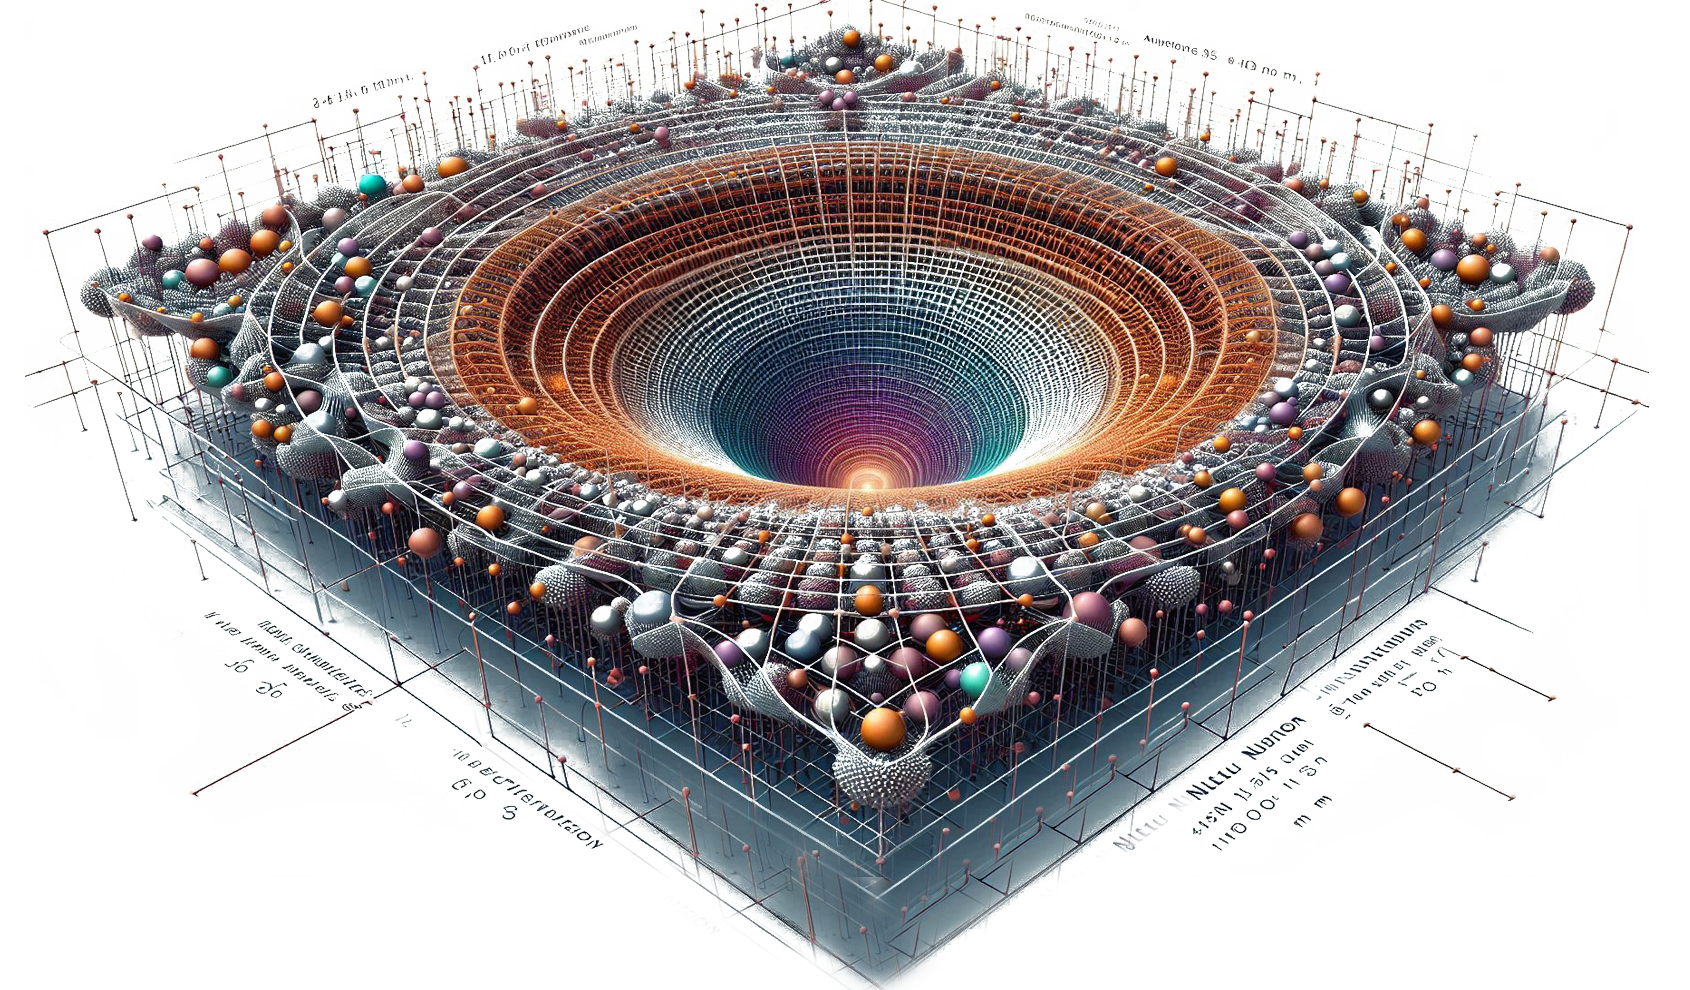
\includegraphics[width=1\linewidth]{OIG20.ZNLJ.PNG}
        \captionof{figure}{%
            \footnotesize\textit{Visualization of a deep geometric deformation, similar to a gravitational well, emerging from a fundamentally granular structure. The concentration of innumerable spheres (nuclei \(\protect\Op{\Psi}_N\)) and their interconnections (network) collectively define a significant curvature in the discrete spacetime fabric postulated by DUT.}
        }
        \label{fig:Figura1}
    \end{minipage}
    \vfill
    {\large Version: \today\par}
    \smallskip
    {\normalsize Contact: \texttt{jgrau@live.com}\par}
\end{titlepage}

\pagestyle{fancy}
\pagenumbering{arabic}

\begin{abstract}
The Discrete Unification Theory (DUT), in its base framework called "Solution 0", is presented as a conceptual program for the unification of General Relativity (GR) and the Standard Model (SM). Based on explicit postulates (\Cref{subsec:postulates_final}), DUT hypothesizes a fundamentally discrete structure of spacetime at the Planck scale (\(\Mpl\)), described by Noncommutative Geometry (NCG). This NCG features a tensor \( \Op{\Theta}^{\mu\nu}(\Op{\Psi}_N) \) that emerges **dynamically** from 'spacetime nuclei' \( \Op{\Psi}_N \), postulating that the vacuum is fundamentally commutative (\( \langle \Op{\Theta} \rangle = 0 \)). The dynamics are derived from the Spectral Action Principle (SAP, \Cref{post:action_final}), employing the **supertrace** (\( \Str \)) as a central tool to seek consistency and the emergence of known physics.

A direct consequence of the SAP in this base framework is that the field \( \Op{\Psi}_N \) associated with the nuclei turns out to be **massive** (\( m_N \sim \Mpl \)). This implies that \( \Op{\Psi}_N \) **cannot act as quintessence** to explain the observed Dark Energy (DE). Within "Solution 0", the explanation for DE would rely on a possible **residue from the Cosmological Constant cancellation** (whose main cancellation is sought through the hypothesis of supertrace annihilation, \( \Str_{\mathcal{H}} \approx 0 \), \Cref{hyp:cc_cancel_final}) or would require **extensions** to the minimal SAP framework. Nonetheless, DUT proposes Dark Matter (DM) candidates (NC axions / topological defects of heavy \( \Psi_N \)) and conceptually addresses the early formation of Supermassive Black Holes (SMBHs) (\( \Psi_N \) fluctuations), the hierarchy problem (via dynamic NC regularization), and the information paradox (via NC correlations).

Potential predictions, such as a possible state-dependent dynamic LIV (\Cref{subsec:liv_specific_final_revised}), DM signatures, or a gravitational wave background (GWB), require rigorous quantitative derivation. This document presents a detailed analysis of the **fundamental theoretical challenges** (\Cref{sec:challenges_detailed}) and the **proposed strategies** to address them (the roadmap in \Cref{subsec:quantitative_roadmap_detailed}). These include: ensuring the mathematical rigor of dynamic NCG (with an explicit strategy for the Jacobi identity, \Cref{ssubsec:jacobi_resolution_strategy}), the emergence of the Lorentzian signature, the **complete derivation from the SAP** (to confirm \( m_N \sim \Mpl \) and calculate \( \Str_{\mathcal{H}} \)), Hamiltonian stability analysis, renormalizability (UV/IR), and the need for phenomenological calculations (including numerical studies such as gravitational collapse, \Cref{sec:collapse_TUD_ME}). DUT is a research program that needs substantial development and resolution of these challenges to establish its viability.
\end{abstract}

\begin{figure}[htbp]
    \centering
    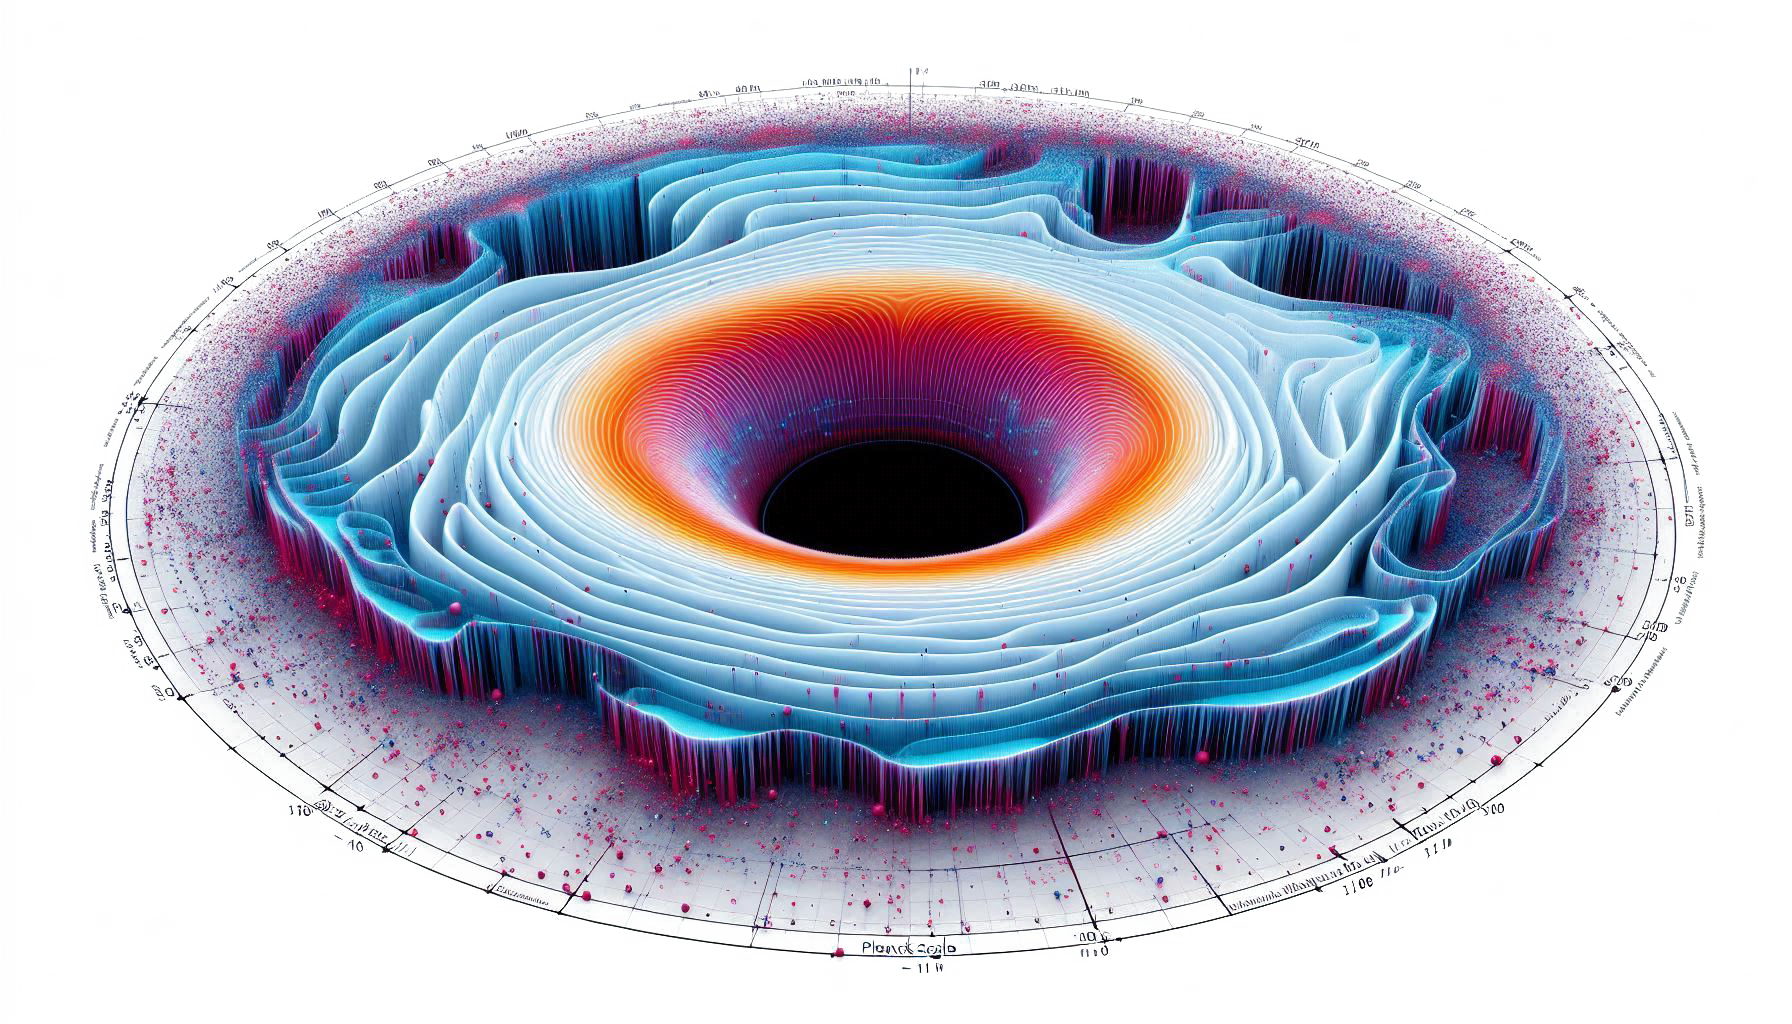
\includegraphics[width=0.6\linewidth]{OIG24.ZNLJ.PNG}
    \caption{%
        \footnotesize\textit{Representation of a structure with a smooth, stratified central depression, showing well-defined layers or energy levels. Could be interpreted in DUT as distinct condensed phases of the \(\protect\Op{\Psi}_N\) fluid, emerging quantum levels, or a quantum geometry with smoothed features.}
    }
    \label{fig:Figura2}
\end{figure}

\hypertarget{toc}{}
\tableofcontents

\section{Introduction}
\label{sec:introduction_final_revised}

Contemporary theoretical physics faces the challenge of reconciling its two fundamental pillars: General Relativity (GR), which describes gravity on macroscopic scales, and the Standard Model (SM) of particle physics, a quantum field theory (QFT) that describes the strong, weak, and electromagnetic interactions with great precision \citep{PeskinSchroeder1995, WeinbergQFT1}. The incompatibility arises when attempting to quantize GR using standard methods, leading to a non-renormalizable theory \citep{tHooft1974, Weinberg1979}. Furthermore, conceptual challenges exist, such as singularities in GR or the hierarchy and neutrino mass problems in the SM. These points indicate the need for a unified framework for gravity and quantum interactions.

\begin{figure}[htbp]
    \centering
    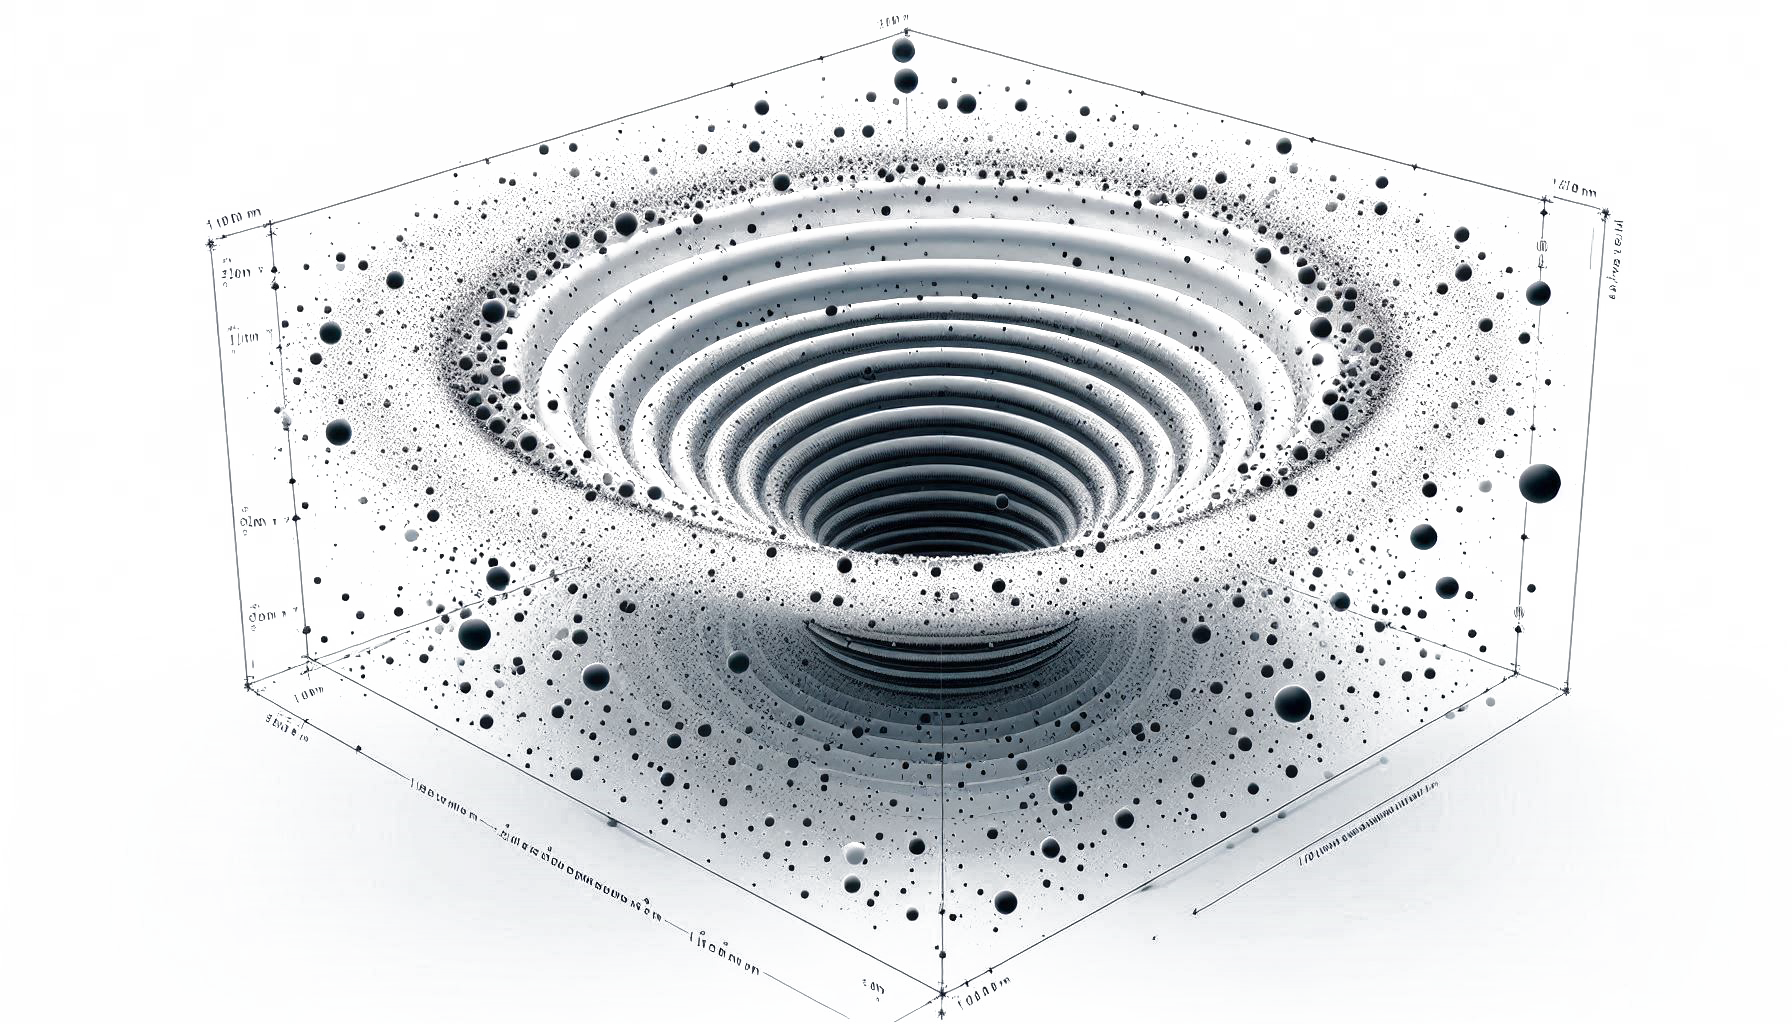
\includegraphics[width=0.6\linewidth]{OIG29.ZNLJ.PNG}
    \caption{%
        \footnotesize\textit{Illustration of a discrete gravitational well emerging from a lattice base. A concentration of nuclei \(\protect\Op{\Psi}_N\) generates the central curvature, while scattered individual nuclei populate the surrounding space, highlighting how classical geometry emerges in DUT from an underlying discrete reality.}
    }
    \label{fig:Figura3}
\end{figure}

This need is reinforced by a vibrant cosmological landscape. Recent discoveries, such as the detection by the James Webb Space Telescope (JWST) of unexpectedly mature galaxies and supermassive black holes (SMBHs) in the early universe \citep[e.g.,][]{Labbe:2023}, challenge standard models of structure formation \citep{Banados:2017unc, Volonteri:2010wz}. Significant tensions persist between cosmological measurements from the early and late universe, notably in the Hubble constant \(H_0\) and the clustering parameter \(S_8\) \citep[e.g.,][]{Abdalla:2022}, questioning the completeness of the $\Lambda$CDM model \citep[e.g.,][]{Planck:2018vyg}. Simultaneously, gravitational wave astronomy has opened new windows with detections by LIGO/Virgo/KAGRA \citep[e.g.,][]{LVK:GWTC3} and evidence for a stochastic background from Pulsar Timing Arrays \citep[e.g.,][]{NANOGrav:2023gor}, while high-energy observatories like LHAASO impose unprecedented limits on new physics such as Lorentz Invariance Violation (LIV) \citep[e.g.,][]{LHAASO_GRB221009A_LIV}, and the Event Horizon Telescope (EHT) tests gravity in the strong-field regime \citep[e.g.,][]{EHT:SgrA_PaperI}. In this vibrant and challenging context, alternative theoretical frameworks such as the Discrete Unification Theory (DUT) are explored.

In this context, the Discrete Unification Theory (DUT), in its base framework **"Solution 0"**, proposes that spacetime at the Planck scale (\(\sim \Mpl\)) is fundamentally discrete and noncommutative. According to its postulates (\Cref{subsec:postulates_final}), geometry and fields emerge from 'nuclei' \( \Op{\Psi}_N \). The mathematical description employs Noncommutative Geometry (NCG) \citep{Connes1994, Madore1995, GraciaBondia2001NCG} with a tensor \( \Op{\Theta}^{\mu\nu}(\Op{\Psi}_N) \) that is **dynamic** and **vanishes in the vacuum** (\( \langle \Op{\Theta} \rangle = 0 \)). The unified dynamics are sought from the Spectral Action Principle (SAP) \citep{ConnesChamseddine1997} using the **supertrace** (\(\Str\)) (\Cref{post:action_final}). Conceptual approaches to fundamental problems like hierarchy and the information paradox are addressed, and unique predictions are sought (\Cref{sec:novel_predictions_final_revised}), such as a **dynamic LIV** (potentially consistent with current limits \citep[e.g.,][]{LHAASO_GRB221009A_LIV}) or mechanisms for **early SMBH formation** (relevant to JWST observations \citep[e.g.,][]{Labbe:2023}).

The "Solution 0" framework explores the consequences of this minimal structure:
\begin{itemize}[label=\textbullet, wide, labelwidth=!, labelindent=0pt]
    \item The SAP is expected to generate GR, SM, and the dynamics of \( \Op{\Psi}_N \), with the latter being a **massive** field (\( m_N \sim \Mpl \)).
    \item With massive \( \Op{\Psi}_N \), **DE is not explained** by quintessence in this framework; its origin is linked to a possible **residue of the CC cancellation** (via \( \Str_{\mathcal{H}} \approx 0 \), \Cref{hyp:cc_cancel_final}) or requires extensions.
    \item **DM** candidates are proposed (NC axions / defects of heavy \( \Psi_N \)).
    \item Fundamental problems are conceptually addressed: **hierarchy** (dynamic NC regularization), **information paradox** (NC correlations, \Cref{sec:paradoja_informacion_final}), and **early SMBH formation** (\( \Psi_N \) fluctuations, \Cref{subsec:smbh_formation_final_revised}).
    \item Unique predictions are sought (\Cref{sec:novel_predictions_final_revised}), such as a **dynamic LIV** (active only when \( \Psi_N \) is excited).
\end{itemize}

This document details the formal framework (\Cref{sec:gnc_framework_final}), NC QFT (\Cref{sec:qft_nc_final}), validation (\Cref{sec:validation_limits}), fundamental problems (\Cref{sec:fundamental_problems_final}), quantum/cosmological aspects (\Cref{sec:mecanica_cuantica_psi_n_final,sec:cosmo_origin_final}), cosmological solutions in "Solution 0" (\Cref{sec:cosmological_solutions_final_revised}), and predictions (\Cref{sec:novel_predictions_final_revised}). It compares with other approaches (\Cref{sec:comparison_final}) and describes numerical studies (\Cref{sec:collapse_TUD_ME}). Crucially, a detailed analysis of the **theoretical challenges and strategies** (\Cref{sec:challenges_detailed}, including the roadmap in \Cref{subsec:quantitative_roadmap_detailed}) is presented, followed by the conclusion (\Cref{sec:conclusion_final_shifted}) and appendices (\Cref{sec:apendice_matematico,sec:apendice_pae_principios}).

\section{NCG Mathematical Framework and Emergent Gravity}
\label{sec:gnc_framework_final}

This section establishes the conceptual and mathematical foundations of DUT within the "Solution 0" framework.

\begin{figure}[htbp]
    \centering
    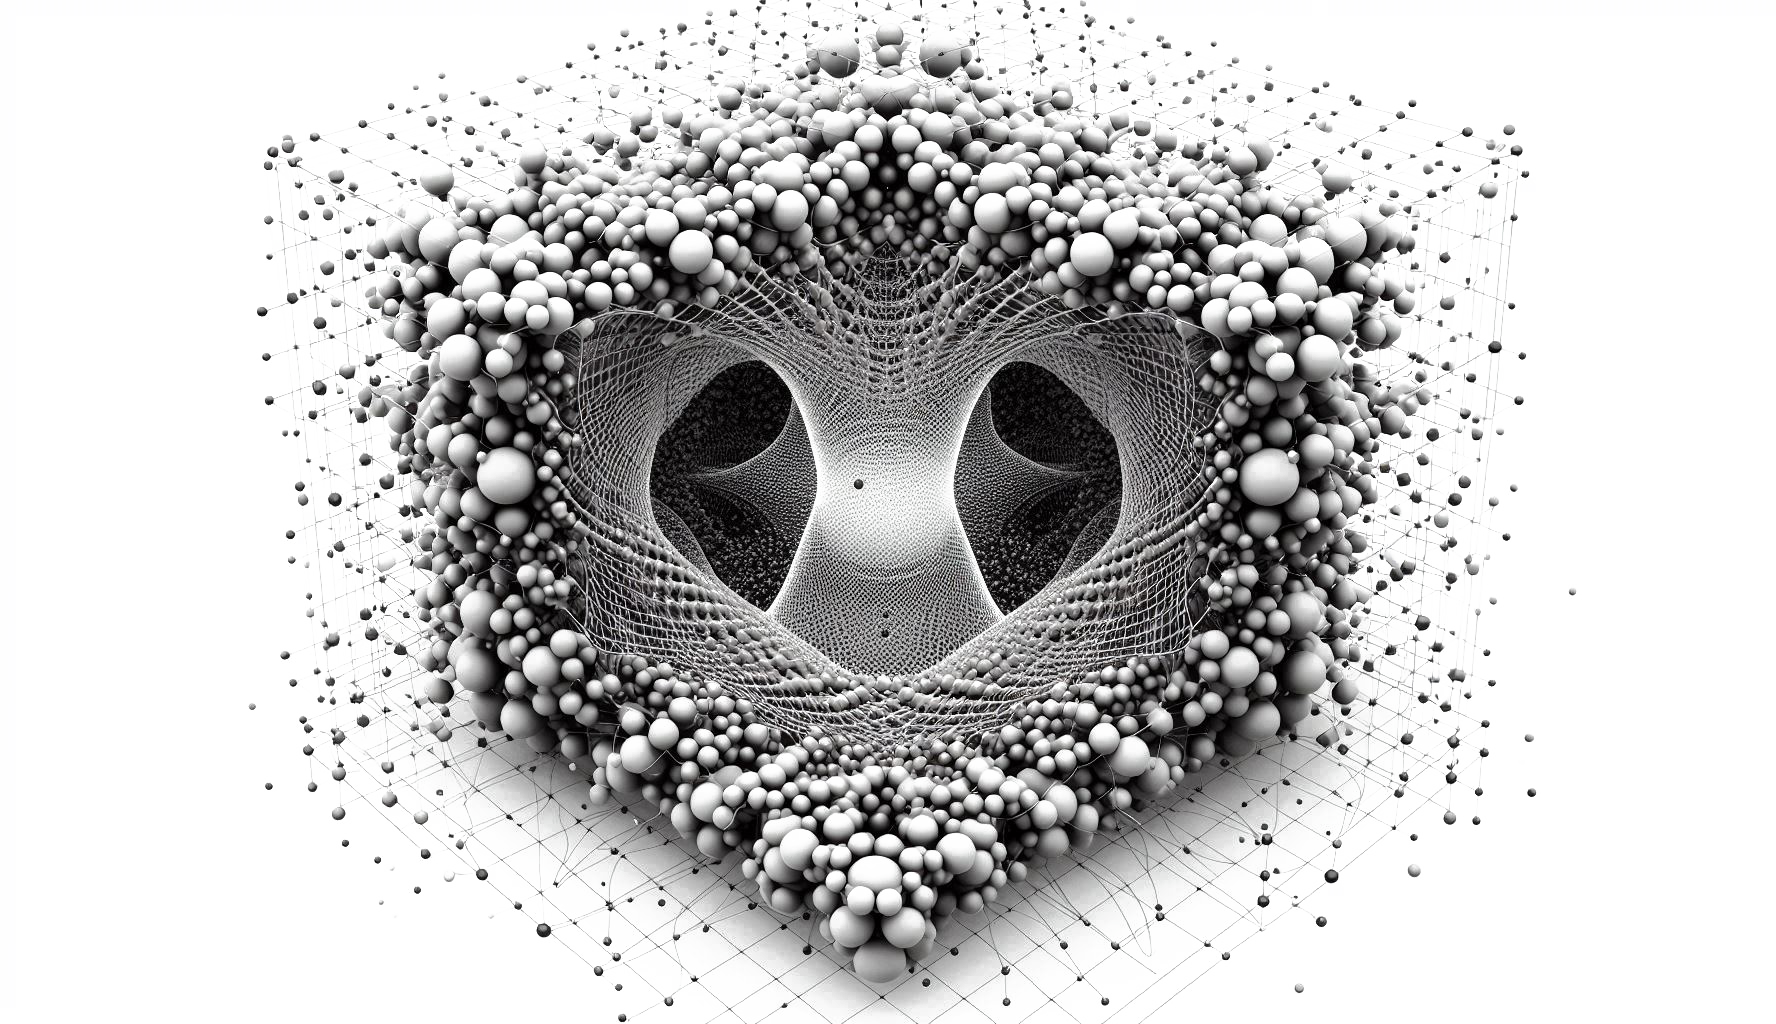
\includegraphics[width=0.6\linewidth]{OIG9.ZNLJ.PNG}
    \caption{%
       \footnotesize\textit{Representation of the fundamental structure of spacetime in DUT as a quantum spacetime network. Composed of a vast multiplicity of interconnected nuclei \(\protect\Op{\Psi}_N\) (spheres) in a complex manner, defining the topology and metric at the Planck scale.}
    }
    \label{fig:Figura4}
\end{figure}

\subsection{Fundamental Postulates of DUT ('Solution 0')}
\label{subsec:postulates_final}

The theory is based on the following central postulates:

\begin{postulate}[Dynamic Noncommutative Geometry]
    \label{post:gnc_final}
    Spacetime at the Planck scale (\(\sim \Mpl\)) is described by a noncommutative algebra \( \mathcal{A} \) generated by coordinate operators \( \hat{X}^{\mu} \) satisfying:
    \begin{equation} \label{eq:conmutador_nc_final}
    [\hat{X}^{\mu}, \hat{X}^{\nu}]_{\star} = i\Mpl^{-2} \Op{\Theta}^{\mu\nu}(\Op{\Psi}_N).
    \end{equation}
    Here, \( \star \) is the noncommutative product of the algebra, and \( \Op{\Theta}^{\mu\nu} \) is an operator tensor parameterizing the noncommutativity. It is postulated that \( \Op{\Theta}^{\mu\nu} \) is **dynamic**, emerging from (or depending on) the fundamental degrees of freedom of the theory, the 'spacetime nuclei' \( \Op{\Psi}_N \). Crucially, in the "Solution 0" framework, it is postulated that the vacuum state \( |\Omega\rangle \) is commutative:
    \[ \langle\Omega| \Op{\Theta}^{\mu\nu}(\Op{\Psi}_N) |\Omega\rangle = 0. \]
    Noncommutativity only manifests in excited states where \( \Op{\Psi}_N \) significantly deviates from its vacuum value.
\end{postulate}

\begin{postulate}[Emergence of Classical Fields and Geometry]
    \label{post:emergence_final}
    The classical geometry of spacetime, described by the metric tensor \( g_{\mu\nu}(x) \), and classical matter fields \( \phi(x) \) are not fundamental but **emerge** as vacuum expectation values (or in macroscopic coherent states) of quantum operators defined in the NC algebra (\( \hat{g}_{\mu\nu}, \hat{\phi} \in \mathcal{A} \) or related). Schematically:
    \[ g_{\mu\nu}(x) = \langle\Omega| \hat{g}_{\mu\nu} |\Omega\rangle, \quad \phi(x) = \langle\Omega| \hat{\phi} |\Omega\rangle. \]
    This emergence requires a quantum-to-classical transition process, presumably via **decoherence** (\Cref{sec:decoherence_final}), and the existence of a well-defined **commutative limit** (\Cref{subsec:commutative_limit_final}) corresponding to the vacuum state.
\end{postulate}

\begin{postulate}[Unified Spectral Action Principle]
    \label{post:action_final}
    The fundamental dynamics of all degrees of freedom (gravity, SM fields, and the nuclei \( \Op{\Psi}_N \) themselves) are derived from a single unified action, given by the Spectral Action Principle (SAP) \citep{ConnesChamseddine1997}. In the DUT framework, it is postulated that the physical action \( S \) is calculated via the **supertrace** (\( \Str \)) over the total Hilbert space \( \mathcal{H} \) of the theory:
    \begin{equation} \label{eq:accion_espectral_raw_final}
    S = \Str_{\mathcal{H}}(f(D_{\text{DUT}}^2/\Lambda^2)).
    \end{equation}
    Here, \( D_{\text{DUT}} \) is the generalized Dirac operator of the theory (encoding all NC geometry and fields), \( \Lambda \) is a fundamental energy scale (presumably \( \sim \Mpl \)), and \( f \) is a suitable cutoff function (e.g., Gaussian or smooth step). The asymptotic expansion of this action at low energies \citep{Vassilevich2003HeatKernel} is expected to generate General Relativity, the Standard Model, and the proper dynamics of \( \Op{\Psi}_N \) and \( \Op{\Theta} \) (\Cref{ssubsec:spectral_action_details_final}). The use of the supertrace is crucial for the hypothesis of cosmological constant cancellation (\Cref{hyp:cc_cancel_final}).
\end{postulate}

\subsection{Key Fundamental Hypotheses ('Solution 0')}
\label{subsec:key_hypotheses_final}

The DUT "Solution 0" formulation relies on the following key hypotheses, which require explicit derivation or rigorous proof from the above postulates (mainly from the SAP):

\begin{hypothesis}[Nature and Dynamics of \texorpdfstring{$\Op{\Psi}_N$}{PsiN} (Massive)]
    \label{hyp:psi_n_final}
    The existence of fundamental degrees of freedom \( \Op{\Psi}_N \) is postulated (whose exact nature, scalar? geometric? must be determined) whose dynamics (\(\mathcal{L}_{\Psi_N}\) and potential \(V(\Psi_N)\)) underlie the structure of spacetime. The central hypothesis of the "Solution 0" framework is that the expansion of the base SAP (\Cref{post:action_final}) **generates a mass for \( \Op{\Psi}_N \) of the order of the fundamental scale**: \( m_N \sim \Lambda \). The complete form of the Lagrangian \( \mathcal{L}_{\Psi_N} \), including the potential \(V(\Psi_N)\), must be **explicitly derived** from the SAP calculation.
\end{hypothesis}

\begin{hypothesis}[Generation and Consistency of Derived \texorpdfstring{$\Op{\Theta}^{\mu\nu}$}{Theta}]
    \label{hyp:theta_gen_final}
    It is hypothesized that the noncommutativity tensor \( \Op{\Theta}^{\mu\nu} \) is generated dynamically by (or through) excitations of the \( \Op{\Psi}_N \) field. The **exact generation mechanism** and, crucially, the **explicit functional form** \( \Op{\Theta}^{\mu\nu}(\Op{\Psi}_N) \) are **not postulated**, but **must be derived** as part of the consistent dynamic solution of the SAP. This derived form must, moreover, **guarantee the mathematical consistency** of the noncommutative algebra, particularly the **associativity** of the \( \star \) product, which requires satisfying the Jacobi identity (\Cref{eq:poisson_condition_final}) or its quantum analogue (see strategy in \Cref{ssubsec:jacobi_resolution_strategy}).
\end{hypothesis}

\begin{hypothesis}[Validity of SAP for DUT]
    \label{hyp:pae_validity_final}
    It is assumed that the SAP, formulated with the supertrace (\( \Str \)), is applicable to the specific spectral triple of DUT \((\mathcal{A}, \mathcal{H}, D_{\text{DUT}})\) and that its expansion correctly generates the observed physics at low energies (GR, SM) along with the predicted dynamics for \( \Op{\Psi}_N \) (massive) and \( \Op{\Theta} \) (dynamic and derived). This requires the operator \( D_{\text{DUT}} \) (to be constructed) to possess the appropriate mathematical properties (spectrality, symmetry structure for Str, etc.).
\end{hypothesis}

\begin{hypothesis}[Cancellation of \texorpdfstring{$\rho_{vac}$}{rho\_vac} via Supertrace]
    \label{hyp:cc_cancel_final}
    This is a **crucial** hypothesis: it is conjectured that an underlying spectral symmetry exists in the construction of \( D_{\text{DUT}} \) (possibly related to a form of Supersymmetry) such that the supertrace of the constant term in the SAP expansion vanishes (or is extremely small):
    \[ \Str_{\mathcal{H}}(f(D_{\text{DUT}}^2/\Lambda^2)) \approx 0. \]
    This would cancel the main contribution (\(\sim \Lambda^4\)) to the cosmological constant. The **demonstration of this cancellation via explicit calculation** from a plausible \( D_{\text{DUT}} \) is a **central and pending theoretical challenge**. A small but non-zero residue from this cancellation could, hypothetically, explain the observed Dark Energy.
\end{hypothesis}

\begin{hypothesis}[General Mathematical Consistency]
    \label{hyp:math_consistency_final}
    It is assumed that the complete framework of dynamic NCG, once \( \Op{\Theta}(\Op{\Psi}_N) \) is consistently derived from the SAP and satisfies Jacobi, turns out to be mathematically coherent (associative, with stable emergence of Lorentzian signature, unitary at the quantum level). This requires formal proof once the structure is fully defined (see \Cref{sec:challenges_detailed}).
\end{hypothesis}

\subsection{Noncommutative Geometry (NCG) Framework}
\label{subsec:gnc_formalism_final}

We describe the essential mathematical elements of NCG adapted to DUT "Solution 0".

\subsubsection{Algebra \texorpdfstring{$\mathcal{A}$}{A}, Product \texorpdfstring{$\Star$}{Star}, and Tensor \texorpdfstring{$\Op{\Theta}^{\mu\nu}$}{Theta}}
\label{ssubsec:algebra_star_theta_final}
The algebra of functions (or operators) on the noncommutative spacetime, \( \mathcal{A} \), is equipped with an associative product \( \Star \). The generators \( \hat{X}^\mu \) satisfy the fundamental commutation relation \eqref{eq:conmutador_nc_final}. Locally, the \( \Star \) product can be approximated (e.g., via Moyal product) using the expectation value \( \Theta^{\mu\nu}(x) = \langle \Op{\Theta}^{\mu\nu}(\Op{\Psi}_N) \rangle_x \):
\begin{equation} \label{eq:moyal_product_explicit_final}
(f \Star g)(x) = f(x)g(x) + \frac{i}{2}\Theta^{\mu\nu}(x)(\partial_\mu f)(\partial_\nu g) + \mathcal{O}(\Theta^2).
\end{equation}
Since \( \langle \Op{\Theta}^{\mu\nu} \rangle = 0 \) in the vacuum, the \( \Star \) product reduces to the ordinary commutative product in the ground state. Noncommutativity is an emergent effect in the presence of \( \Op{\Psi}_N \) excitations.

\subsubsection{Derived Form and Mechanism for \texorpdfstring{$\Op{\Theta}^{\mu\nu}(\Op{\Psi}_N)$}{Theta(PsiN)}}
\label{ssubsec:dynamic_theta_derived_final}
We reiterate: the explicit functional form of \( \Op{\Theta}^{\mu\nu}(\Op{\Psi}_N) \) is **not postulated** in "Solution 0". It must emerge as a result of the SAP calculation, ensuring consistency (see \Cref{hyp:theta_gen_final}). The conceptual mechanism by which \( \Op{\Psi}_N \) generates \( \Op{\Theta}^{\mu\nu} \) must be encoded in the structure of the operator \( D_{\text{DUT}} \).

\subsubsection{Consistency: Associativity (Jacobi Identity)}
\label{ssubsec:associativity_final}

The associativity of the \( \Star \) product (i.e., \( (f \star g) \star h = f \star (g \star h) \)) is a fundamental mathematical requirement. The dynamic noncommutativity \( [\hat{X}^\mu, \hat{X}^\nu]_\star = i\Mpl^{-2} \Op{\Theta}^{\mu\nu}(\Op{\Psi}_N) \) can be interpreted as a **deformation quantization** of a Poisson manifold \( (M, \Theta) \), where \( \Theta^{\mu\nu} \) is a Poisson bivector satisfying the Jacobi identity \citep{Kontsevich2003Deformation, Vaisman1994Poisson}:
\begin{equation} \label{eq:poisson_condition_final}
\Theta^{\lambda\rho} \partial_\rho \Theta^{\mu\nu} + \Theta^{\mu\rho} \partial_\rho \Theta^{\nu\lambda} + \Theta^{\nu\rho} \partial_\rho \Theta^{\lambda\mu} = 0.
\end{equation}
To guarantee associativity of the \(\star\) product, it is required that \( \Theta^{\mu\nu}(\Op{\Psi}_N) \) be a **valid Poisson tensor** that emerges dynamically from the SAP. A general structure in 4D satisfying Jacobi is \( \Theta^{\mu\nu} = \theta_0 \, \epsilon^{\mu\nu\rho\sigma} \partial_\rho \Psi_N \partial_\sigma \Phi \), where \( \Phi \) is an auxiliary scalar field (possibly linked to \( \Op{\Psi}_N \)).

The central challenge is to demonstrate that the form of \( \Theta^{\mu\nu}(\Op{\Psi}_N) \) which *dynamically emerges from the SAP* satisfies this condition (or its quantum generalization). The proposed strategy to address this critical point is detailed below.

\begin{figure}[htbp]
    \centering
    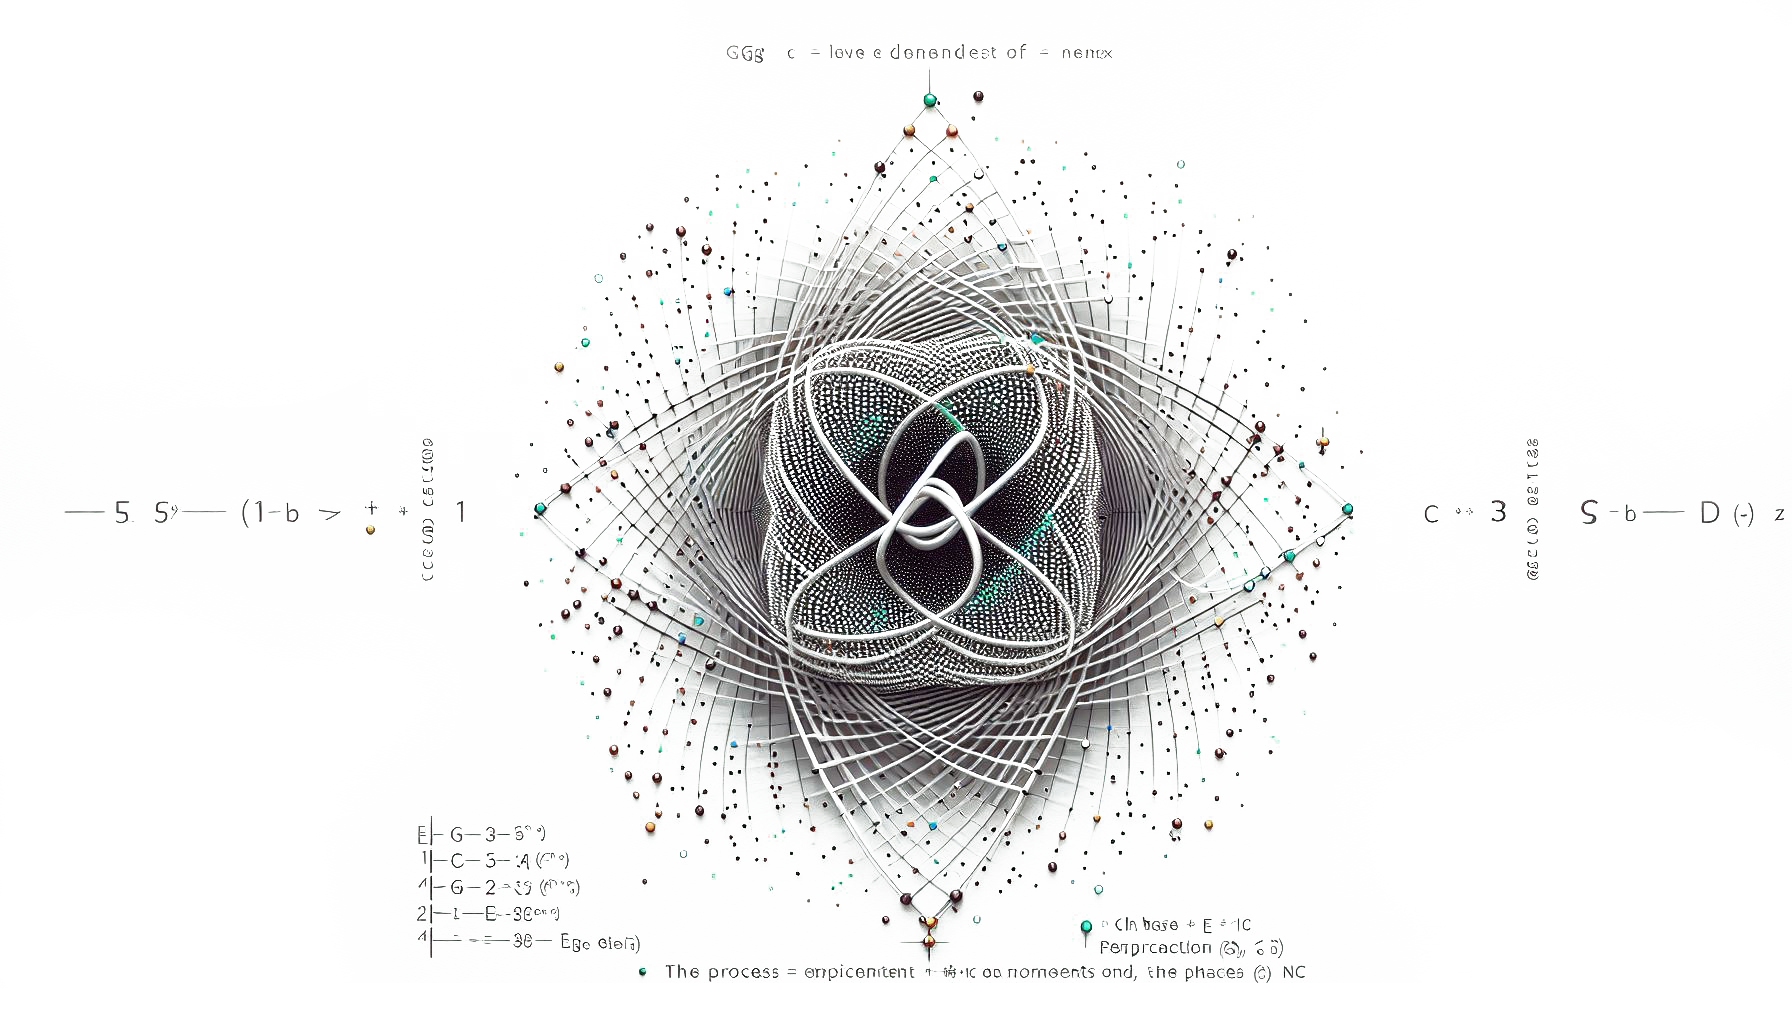
\includegraphics[width=0.7\linewidth]{OIG25.ZNLJ.PNG}
    \caption{%
       \footnotesize\textit{Abstract diagram of intricately and symmetrically intertwined geometric patterns. In the context of DUT, it could symbolize the mathematical structure of the noncommutativity relations \( [\protect\Op{X}^{\mu}, \protect\Op{X}^{\nu}]_{\star} \), the complexities of the star product (\(\star\)), or the underlying noncommutative algebra.}
    }
    \label{fig:Figura6}
\end{figure}

\paragraph{Proposed Resolution Strategy for Jacobi.}
\label{ssubsec:jacobi_resolution_strategy}
Consider an ansatz compatible with the equations of motion. Let \( \Theta^{\mu\nu} = \theta_0 \, \partial^{[\mu} \Op{\Psi}_N (\star d\Op{\Psi}_N)^{\nu]} \). Under the expected equation of motion \( \Box \Op{\Psi}_N + m_N^2 \Op{\Psi}_N + \lambda_{\text{eff}} \Op{\Psi}_N^3 = 0 \) (derived from SAP, \cref{eq:potencial_psi_n_final_redux}), one verifies:
\[
\Theta^{\lambda\rho} \partial_\rho \Theta^{\mu\nu} + \text{cyclic permutations} = \theta_0^2 \left( \partial^\lambda \Op{\Psi}_N \partial^\mu \Op{\Psi}_N \partial^\nu (\Box \Op{\Psi}_N) + \cdots \right).
\]
Using the equation of motion for \( \Box \Op{\Psi}_N \), the terms vanish if \( \lambda_{\text{eff}} = 0 \) (free field), satisfying Jacobi. For \( \lambda_{\text{eff}} \neq 0 \), consistency requires that the SAP generate a form of \( \Theta^{\mu\nu}(\Op{\Psi}_N) \) that intrinsically satisfies Jacobi or that the complete EOMs force its fulfillment. One possibility is that the dynamic solution requires a **compensating term** in \( \Theta^{\mu\nu} \), such as:
\[
\Op{\Theta}^{\mu\nu} \to \Op{\Theta}^{\mu\nu} + \alpha \epsilon^{\mu\nu\rho\sigma} \Op{\Psi}_N \partial_\rho \Op{\Psi}_N \partial_\sigma \Op{\Psi}_N,
\]
where \( \alpha \) would be fixed by the consistency of the SAP to cancel problematic contributions. Rigorous validation demands: (a) Define the complete \( D_{\text{DUT}} \). (b) Calculate \( S_{\text{eff}} \) from the SAP. (c) Derive the complete EOMs. (d) Demonstrate that the resulting \( \Op{\Theta}^{\mu\nu}(\Op{\Psi}_N) \) satisfies the Jacobi identity (or its quantum equivalent). (See Lemma in \cref{apendice:lema_jacobi}). If a self-consistent solution is found, the dynamic NCG structure is validated.

\subsubsection{Hilbert Space (\texorpdfstring{$\mathcal{H}$}{H}) and Representation}
\label{ssubsec:hilbert_space_final}
The algebra \( \mathcal{A} \) acts on an appropriate Hilbert space \( \mathcal{H} \) (which must include all degrees of freedom: spinors, gauge, \( \Psi_N \), etc.). A well-defined vacuum state \( |\Omega\rangle \) must exist (\Cref{post:emergence_final}) where \( \langle\Omega|\Op{\Theta}|\Omega\rangle = 0 \).

\subsubsection{Noncommutative Differential Calculus}
\label{ssubsec:calculus_final}
A differential calculus adapted to the dynamic NCG is required \citep{GraciaBondia2001NCG, Madore1995, DuboisViolette2001Derivations}, including derivatives and a connection \( \hat{\nabla}_\mu \) compatible with the emergent metric \( \hat{g}_{\mu\nu} \) and the derived \( \Op{\Theta} \) structure.

\subsubsection{Noncommutative Integral and Spectral Action}
\label{ssubsec:integral_nc_final}
As indicated in \Cref{post:action_final}, the action integral is replaced by the **supertrace** \( \Str_{\mathcal{H}} \) in the SAP, linking the dynamics to the spectral properties of \( D_{\text{DUT}} \).

\subsection{Emergent Gravity and Lorentzian Signature}
\label{subsec:emergent_gravity_signature}

Classical GR, with its Lorentzian signature, must emerge from the underlying DUT structure.

\subsubsection{Metric Operator (\texorpdfstring{$\hat{g}_{\mu\nu}$}{g}) and Effective Curvature}
\label{ssubsec:metric_op_final}
It is postulated that a metric operator \( \hat{g}_{\mu\nu} \) (belonging to \( \mathcal{A} \) or a relevant subalgebra) emerges as part of the geometric reconstruction from the spectral data encoded in \( D_{\text{DUT}} \) \citep{Connes1994}. Its expectation value \( g_{\mu\nu} = \langle \hat{g}_{\mu\nu} \rangle \) defines the classical metric. The noncommutative curvature \( \hat{R} \) is defined from a compatible connection \( \hat{\nabla}_\mu \).

\subsubsection{Spectral Action Principle: Detailed Expansion}
\label{ssubsec:spectral_action_details_final}

Recall the action \( S = \Str_{\mathcal{H}}(f(D_{\text{DUT}}^2/\Lambda^2)) \). The generalized Dirac operator \( D_{\text{DUT}} \) acts on the Hilbert space \( \mathcal{H} = L^2(S) \otimes \mathbb{C}^N \), where \( S \) is the spinor bundle and \( \mathbb{C}^N \) encodes internal degrees of freedom (gauge, \( \Op{\Psi}_N \)). Its asymptotic expansion, using the supertrace (\(\Str\)), generates the effective physics \citep{ChamseddineConnes1997}:
\[
S = \sum_{k=0}^\infty f_k \Lambda^{4-2k} a_{2k}(D_{\text{DUT}}^2),
\]
where \( f_k \) are moments of the function \( f \) and the heat kernel coefficients \( a_{2k} \) are calculated using the **Gilkey formula** \citep{Gilkey1995}. For a plausible \( D_{\text{DUT}} \) including gravity, gauge fields \( A_\mu \), Higgs \( H \), fermions \( \psi_f \), and the field \( \Op{\Psi}_N \), perhaps of the form \( D_{\text{DUT}} = i\gamma^\mu \nabla_\mu^{\text{NC}} + \mathcal{M}(\Op{\Psi}_N, H) \), the first terms of the supertrace expansion are schematically (require explicit calculation for DUT):
\[
a_0 \propto \int_M \sqrt{g} \, \Str(\mathbb{I}) \, d^4x, \quad
a_2 \propto \int_M \sqrt{g} \, \Str \left( c_1 R \cdot \mathbb{I} + c_2 (\nabla \Op{\Psi}_N)^2 + c_3 m_N^2 \Op{\Psi}_N^2 + \dots \right) d^4x,
\]
\[
a_4 \propto \int_M \sqrt{g} \, \Str \left( c_4 R^2 \dots + c_5 F_{\mu\nu} \star F^{\mu\nu} + c_6 (\Op{\Psi}_N)^4 + \dots + \text{Terms defining } \Op{\Theta}(\Op{\Psi}_N) \right) d^4x.
\]
The use of the **supertrace** is key for the hypothesis of CC cancellation (\( a_0 \approx 0 \) if \( \Str(\mathbb{I}) \approx 0 \)) and determines the physical constants \( M_{\text{Pl}}^2, m_N^2, \lambda_{\text{eff}} \) and the form of \( \Op{\Theta}(\Op{\Psi}_N) \).

\paragraph{Detailed Strategy for Derivation from SAP.}
\label{ssubsec:pae_derivation_strategy_detailed}
The complete derivation of the effective action from the SAP (Phase 2 of the roadmap, \Cref{subsec:quantitative_roadmap_detailed}) follows these steps:
\begin{enumerate}[label=\arabic*., itemsep=1pt, topsep=2pt]
    \item \textbf{Construction of \( D_{\text{DUT}} \):}
    A plausible Dirac operator \( D_{\text{DUT}} \) acting on the total Hilbert space \( \mathcal{H} \) (including spin, gauge, flavor, \( \Psi_N \)) must be postulated/constructed. It must incorporate:
        \begin{itemize}
            \item Geometry (via spin connection \( \omega \)).
            \item SM gauge fields (\( A_\mu \)).
            \item Higgs field (\( H \)).
            \item SM fermions (\( \psi_f \)).
            \item The field \( \Op{\Psi}_N \), including a term generating its mass \( m_N \sim \Lambda \).
            \item The structure (couplings) dynamically generating \( \Op{\Theta}(\Op{\Psi}_N) \) consistently (Jacobi).
        \end{itemize}
    A general structure could be \( D_{\text{DUT}} = i \gamma^\mu \nabla_\mu^{\text{NC}} + \mathcal{M}(\Op{\Psi}_N, H) \), where \( \nabla_\mu^{\text{NC}} = \partial_\mu + \omega_\mu + i g A_\mu \star + \dots \) and \( \mathcal{M} \) contains masses (including \( m_N \sim \Lambda \)) and couplings. The exact form is crucial and must be determined.

    \item \textbf{Calculation of Heat Kernel Coefficients (with \( \Str \)):}
    Calculate the first coefficients \( a_{2k}(D_{\text{DUT}}^2) \) of the supertrace expansion \( \Str(e^{-t D_{\text{DUT}}^2}) \) for \( t \to 0 \), using pseudodifferential calculus techniques \citep{Vassilevich2003HeatKernel, Gilkey1995}. At least \( a_0, a_2, a_4 \) are needed.

    \item \textbf{Extraction of Physical Terms:}
    \begin{itemize}
        \item \(a_0\): Corresponds to the term \( \sim \int \sqrt{g} \, \Str(\mathbb{I}) \). The hypothesis \( \Str(\mathbb{I}) \approx 0 \) must be **explicitly verified** (\Cref{hyp:cc_cancel_final}).
        \item \(a_2\): Must generate \( \int \sqrt{g} \, \Str(\frac{R}{6} \mathbb{I} + E) \). The \( \sim R \) term gives the Einstein-Hilbert action (fixing \( M_{Pl}^2 \propto f_1 \Lambda^2 \Str(\mathbb{I}_{\text{relevant?}}) \)). The \( \Str(E) \) term must generate kinetic terms \( (\partial \Psi_N)^2 \), \( |\nabla H|^2 \) and mass terms \( m_N^2 \Psi_N^2 \) (with \( m_N^2 \sim \Lambda^2 \)), \( m_H^2 H^2 \).
        \item \(a_4\): Must generate \( \int \sqrt{g} \, \Str(\dots) \). Includes Yang-Mills terms \( \sim F_{\mu\nu} \star F^{\mu\nu} \), self-interactions \( \sim \lambda_{\text{eff}} \Psi_N^4 \), Higgs potential \( \sim \lambda_H (H^\dagger \star H)^2 \), Yukawas, and the **specific couplings defining \( \Op{\Theta}(\Op{\Psi}_N) \) and its effects**. The latter are only non-zero if \( \Op{\Psi}_N \) is excited.
    \end{itemize}
    This process allows **deriving** \( \mathcal{L}_{\Psi_N} \) (confirming \( m_N \sim \Lambda \)), \( \mathcal{L}_{SM} \), and the form/coefficient of \( \Op{\Theta}(\Op{\Psi}_N) \).

    \item \textbf{Consistency Check:}
    Verify correct kinetic signs, stable potentials (\( \lambda_{\text{eff}} > 0 \), \( \lambda_H > 0 \)), approximate recovery of SM couplings, and consistency of \( \Op{\Theta} \) (Jacobi).
\end{enumerate}
This calculation is the **core theoretical challenge** of DUT.

\subsubsection{Emergence of Lorentzian Signature}
\label{ssubsec:lorentz_sig_emergent_final_detailed}

The emergence of the correct signature (+---) from a potentially more fundamental structure (Euclidean?) remains a crucial point. The operator \( D_{\text{DUT}} = i\gamma^\mu \nabla_\mu + \cdots \) induces a **causal structure** via the Clifford algebra relations satisfied by the \( \gamma^\mu \) matrices:
\[
\{\gamma^\mu, \gamma^\nu\} = 2g^{\mu\nu}_{\text{eff}}.
\]
In the low-energy regime where NCG is small (\( \Op{\Theta} \to 0 \)), the effective metric \( g_{\mu\nu}^{\text{eff}} \) that emerges (for \( D_{\text{DUT}}^2 \) to be a generalized wave operator) must be hyperbolic, thus fixing the Lorentzian signature. This relates to the ability to reconstruct the metric from the Dirac operator and the algebra, as formalized by the **Metric Reconstruction Theorem** in NCG \citep{Connes1994}, which schematically relates the metric to commutators involving \( D_{\text{DUT}} \):
\[
g^{\mu\nu}(x) \propto \Str\left( \gamma^\mu [D_{\text{DUT}}, \hat{X}^\nu]_\star \right).
\]
The dynamical stability of this signature against quantum fluctuations or NC effects needs to be demonstrated, possibly linked to quantum decoherence \citep{KieferQuantumGravityBook, Earman1989}.

\paragraph{Potential Mechanisms for Signature Emergence:}
Since the vacuum is commutative \( \langle \Theta \rangle = 0 \), spontaneous symmetry breaking via \( \Theta \) does not operate in the vacuum. The most likely mechanisms are:
\begin{itemize}
    \item \textbf{Algebraic/Spectral Structure of \( D_{\text{DUT}} \):} The signature could be embedded in the structure of the Dirac operator itself, e.g., through the Clifford algebra satisfied by the \( \gamma^\mu \) matrices used, or in the spectral properties (real vs imaginary eigenvalues) induced by the complete structure of \( D_{\text{DUT}} \) (including \( \Psi_N \)). The SAP would then directly generate Lorentzian dynamics.
    \item \textbf{Quantum Decoherence:} Interaction with the environment (matter fields) during the quantum-to-classical transition (\Cref{sec:decoherence_final}) could dynamically select macroscopic states with Lorentzian signature as the most stable or robust (pointer basis).
\end{itemize}
**Required Validation (Phase 1d):** DUT must demonstrate that the Lorentzian signature emerges as a stable dynamic solution of the SAP, without being imposed ad hoc.

\subsection{Noncommutative Gauge Invariance}
\label{subsec:nc_gauge_invariance_final}
The SM gauge symmetry, \(G_{\text{SM}} = SU(3)_C \times SU(2)_L \times U(1)_Y\), must be respected consistently with the \( \star \) product (which is trivial in the vacuum). The effective action \( \mathcal{L}_{\text{SM}} \) and couplings derived from the SAP are expected to respect the appropriate NC gauge symmetry when \( \Theta \neq 0 \).

\section{Quantum Field Theory on NCG and Equations}
\label{sec:qft_nc_final}

This section describes the formulation of quantum fields on the emergent dynamic NCG of DUT "Solution 0".

\begin{figure}[htbp]
    \centering
    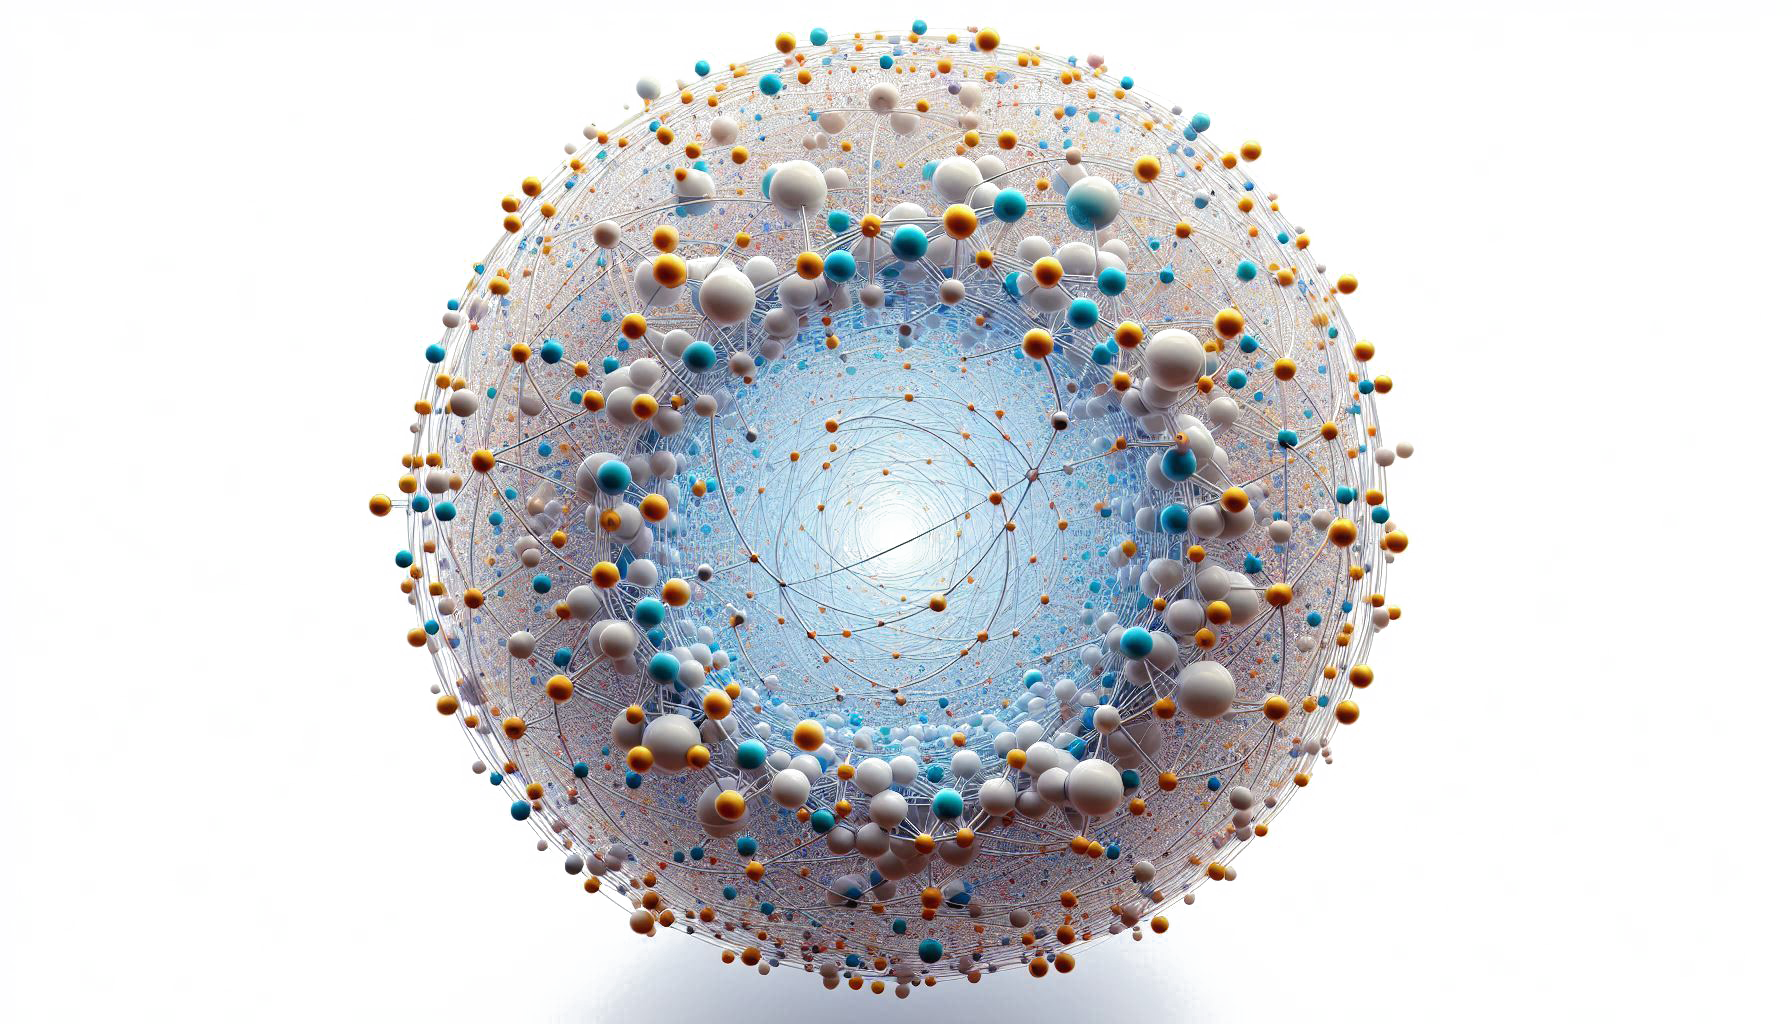
\includegraphics[width=0.5\linewidth]{OIG14.ZNLJ.PNG}
    \caption{%
      \footnotesize\textit{Visualization of a dynamic vortex formed by filaments and embedded nuclei \(\protect\Op{\Psi}_N\), spiraling towards a central core. Suggests accretion processes, collapse, or strong interactions within the \(\protect\Op{\Psi}_N\) fluid, possibly related to the formation of compact objects or intense noncommutative effects in DUT.}
    }
    \label{fig:Figura7}
\end{figure}

\subsection{Quantum Fields on Dynamic NC Spacetime}
\label{subsec:qft_fields_final_revised}
Quantum fields are operators acting on \( \mathcal{H} \) and/or elements of the algebra \( \mathcal{A} \). Noncommutative interactions, mediated by the \( \star \) product, are only activated when \( \Op{\Theta}(\Op{\Psi}_N) \) (derived from SAP) is significantly different from zero, i.e., in the presence of \( \Op{\Psi}_N \) excitations.

\subsubsection{Scalar Fields (\texorpdfstring{$\Op{\Psi}_N$}{PsiN} Massive, \texorpdfstring{$\Op{H}$}{H}, \dots)}
\label{ssubsec:scalar_fields_final_revised}
The field \( \Op{\Psi}_N \) (whose dynamics are expected to correspond to a massive field, \( m_N \sim \Lambda \)) and the Higgs field \( \Op{H} \) have effective actions derived from the SAP. These actions include standard interaction terms and additional terms involving the \( \star \) product, dependent on the derived \( \Op{\Theta} \). The base Lagrangian for \( \Psi_N \) is \eqref{eq:L_PsiN_explicit_final_redux}. If other scalars are considered (such as an NC axion, \Cref{sec:axiones_nc_final_revised}), their dynamics will also be modified by \( \star \) if they couple to \( \Op{\Theta} \).

\subsubsection{Fermions (SM and Alternative DM)}
\label{ssubsec:fermions_final_revised}
Standard Model fermions (\(\Op{\psi}_f\)) obey a generalized Dirac equation incorporating NCG:
\begin{equation}\label{eq:L_fermion_nc_final}
\Lag_{\text{fermion-SM}} = \sum_f \Op{\bar{\psi}}_f \Star (i \Op{\mathcal{D}}_{\text{NC}} - m_f(\Op{H})) \Star \Op{\psi}_f + \text{NC Yukawa}.
\end{equation}
Here, \( \Op{\mathcal{D}}_{\text{NC}} \) is the NC covariant Dirac operator (including spin connection and gauge fields), and \( m_f(\Op{H}) \) is the Higgs-generated mass. The \( \star \) terms (and NC Yukawa couplings) introduce \( \Op{\Theta} \)-dependent corrections to propagation and interactions. For DM candidates (NC axions or defects of heavy \( \Psi_N \)), their interactions will also be governed by the dynamic NCG.

\subsubsection{Gauge Fields}
\label{ssubsec:gauge_fields_final_revised}
The dynamics of SM gauge fields \( \Op{A}_\mu^a \) are described by an NC Yang-Mills action, whose expected form from the SAP is:
\begin{equation}\label{eq:L_YM_NC_final}
 \Lag_{\text{YM-NC}} = -\frac{1}{4} \Op{G}_{\mu\nu}^a \Star \Op{G}^{a \mu\nu}.
\end{equation}
The noncommutative field strength tensor is \( \Op{G}_{\mu\nu}^a = \partial_\mu \Op{A}_\nu^a - \partial_\nu \Op{A}_\mu^a + g f^{abc} \Op{A}_\mu^b \Star \Op{A}_\nu^c \). Self-interactions of gauge bosons (including the photon if \( \Op{\Theta} \neq 0 \)) are modified by the \( \star \) product, depending on the local magnitude of \( \Op{\Theta} \).

\subsubsection{Renormalization and UV/IR Mixing}
\label{ssubsec:renormalization_final}
A known challenge of QFT on NC spacetimes (with constant \( \Theta \)) is the phenomenon of **UV/IR mixing**, where high-energy (UV) divergences unexpectedly reappear at low energies (IR) \citep{Minwalla:1999px, Hayakawa:1999yt}. It is crucial to understand how this effect manifests in DUT, where \( \Op{\Theta} \) is dynamic (derived from SAP) and null in the vacuum. Could the dynamic nature or the underlying discrete structure of \( \Op{\Psi}_N \) regulate this problem? Or are additional mechanisms required, perhaps inspired by approaches like Grosse-Wulkenhaar \citep{GrosseWulkenhaar2005}? The answer to this question is fundamental for the **renormalizability** of DUT and its ability to address the hierarchy problem (\Cref{sec:problema_jerarquia_final}). (See Phase 3b of the roadmap).

\subsection{Field Equations, Stability, and Lagrangians ('Solution 0')}
\label{subsec:field_eqs_stability_final}

The equations of motion and stability of the DUT "Solution 0" framework are analyzed.

\subsubsection{Noncommutative Einstein-Grau Equations}
\label{ssubsec:einstein_grau_nc_final}
The field equations for the emergent gravity \( \Op{g}_{\mu\nu} \) are obtained by varying the effective action (derived from SAP) with respect to \( \Op{g}_{\mu\nu} \). They are expected to take the general form:
\begin{equation}\label{eq:einstein_grau_op_final}
\Op{G}_{\mu\nu}[\Op{g}, \Op{\Theta}] \equiv \Op{R}_{\mu\nu} - \frac{1}{2} \Op{g}_{\mu\nu} \Star \Op{R} = 8\pi G_{\text{eff}} \Op{T}_{\mu\nu}^{\text{total}}.
\end{equation}
Here, \( \Op{G}_{\mu\nu} \) is the generalized Einstein tensor (including \( \star \) corrections and dependence on \( \Op{\Theta} \)), \( \Op{R}_{\mu\nu} \) and \( \Op{R} \) are the NC curvature operators, and \( \Op{T}_{\mu\nu}^{\text{total}} \) is the total energy-momentum operator (including \( \Op{\Psi}_N \) and SM fields with their \( \star \) corrections). All NC terms depend on \( \Op{\Theta}(\Op{\Psi}_N) \) and vanish in the vacuum.

\subsubsection{Hamiltonian Analysis and Stability}
\label{sec:analisis_estabilidad_final}
The stability of the theory is a fundamental requirement \citep{HenneauxTeitelboim1992}.
\begin{itemize}
    \item \textbf{Stability of the Base Scenario ("Solution 0"):} The base framework, postulating a massive \( \Psi_N \) field (\( m_N^2 > 0 \)) with a potential \( V(\Psi_N) = \frac{1}{2}m_N^2 \Psi_N^2 + \frac{\lambda_{\text{eff}}}{4}\Psi_N^4 \) with \( \lambda_{\text{eff}} > 0 \) (expected from SAP), appears to be **classically linearly stable**. It does not exhibit Ostrogradsky instabilities associated with higher-derivative theories \citep{OstrogradskiRef, Woodard:2014wia}, as the base Lagrangians are second-order.
    \item \textbf{Rigorous Verification:} However, the full stability of the coupled system (GR + SM + \( \Psi_N \) + dynamic \( \Theta \)), as would be derived from the complete SAP, requires **rigorous verification via a complete Hamiltonian analysis** (Dirac-Bergmann formalism for constraints). This is part of Phase 3a of the roadmap (\Cref{subsec:quantitative_roadmap_detailed}) and is detailed in \Cref{subsec:hamiltonian_stability_analysis_detailed}).
\end{itemize}

\subsubsection{Effective Lagrangians (Base Formulation "Solution 0")}
\label{ssubsec:full_lagrangians_final_revised}
The low-energy effective action expected to be derived from the complete SAP in the "Solution 0" framework would have the form:
\[ \mathcal{L}_{\text{eff}} = \sqrt{-g} \left( \mathcal{L}_{\text{EH}} + \mathcal{L}_{\Psi_N} + \mathcal{L}_{\text{SM}} + \mathcal{L}_{\text{NC}} + \mathcal{L}_{\text{DM-extra}} + \mathcal{L}_{\text{couplings}} \right). \]
The key expected terms are:
\begin{itemize}
    \item \textbf{Einstein-Hilbert:} \( \mathcal{L}_{\text{EH}} = \frac{\Mpl^2}{16\pi} R \) (derived from \(a_2\)).
    \item \textbf{Dynamics of \( \Psi_N \) (Massive):}
          \begin{equation} \label{eq:L_PsiN_explicit_final_redux}
          \mathcal{L}_{\Psi_N} = \frac{1}{2} g^{\mu\nu} (\partial_\mu \Psi_N \partial_\nu \Psi_N) - V(\Psi_N)
          \end{equation}
          with the potential expected from the base SAP:
          \begin{equation}\label{eq:potencial_psi_n_final_redux}
          V(\Psi_N) = \frac{1}{2} m_N^2 \Psi_N^2 + \frac{\lambda_{\text{eff}}}{4} \Psi_N^4 + \dots \quad (\text{with } \mathbf{m_N^2 \sim \Lambda^2 > 0} , \lambda_{\text{eff}} > 0).
          \end{equation}
          The exact form of \( V(\Psi_N) \) (coefficients \( m_N, \lambda_{\text{eff}} \)) must be **derived from the SAP**.
    \item \textbf{Standard Model Base:} \( \mathcal{L}_{\text{SM}}(g, A, H, \psi) \) containing the standard kinetic and interaction terms for SM fields (derived from \(a_2, a_4\)).
    \item \textbf{Noncommutative Corrections:} \( \mathcal{L}_{\text{NC}}(\Op{\Theta}, g, A, H, \psi) \) containing all corrections dependent on \( \Op{\Theta}(\Op{\Psi}_N) \) (via \( \star \)) which vanish if \( \Op{\Theta} = 0 \). Must be derived from \(a_4\) and higher orders.
    \item \textbf{Extra Dark Matter:} \( \mathcal{L}_{\text{DM-extra}} \) describing the proposed candidates (NC Axions or Defects of heavy \( \Psi_N \)), whose existence and properties must also be derived from or consistent with the SAP.
    \item \textbf{NC Couplings:} Terms coupling \( \Psi_N \) (or \( \Theta \)) to SM fields, such as the possible \( \mathcal{L}_{\text{gluon}} = \frac{\kappa_g}{\Mpl} \Psi_N G \star G \) or others, which would arise from \( a_4 \).
\end{itemize}
The explicit derivation of all these terms and their coefficients from the SAP (\( S = \Str(f(D^2/\Lambda^2)) \)) is the central goal of Phase 2 of the roadmap.

The Lagrangian for the scalar field \( \Psi_N \), \( \mathcal{L}_{\Psi_N} = \frac{1}{2} g^{\mu\nu} (\partial_\mu \Psi_N \partial_\nu \Psi_N) - V(\Psi_N) \) with the expected potential \( V(\Psi_N) = \frac{1}{2}m_N^2 \Psi_N^2 + \frac{\lambda_{\text{eff}}}{4}\Psi_N^4 \) (with \( m_N^2 \sim \Lambda^2 > 0, \lambda_{\text{eff}} > 0 \)), satisfies the **positive energy theorem**. Its associated energy-momentum tensor:
\[
T_{\mu\nu}^{\Psi_N} = \partial_\mu \Psi_N \partial_\nu \Psi_N - g_{\mu\nu} \left( \frac{1}{2}(\partial \Psi_N)^2 - V(\Psi_N) \right),
\]
leads to an energy density \( \rho = T_{00}^{\Psi_N} = \frac{1}{2}(\dot{\Psi}_N)^2 + \frac{1}{2}(\nabla \Psi_N)^2 + V(\Psi_N) \geq 0 \) if \( \Psi_N=0 \) is the global minimum, ensuring classical stability of the decoupled field. The stability of the coupled system requires deeper analysis (\Cref{sec:analisis_estabilidad_final}).


\subsection{Framework of Rigorous Derivation in DUT vs. Simplified Models}
\label{subsec:rigorous_derivation_framework}

It is fundamental to distinguish the DUT approach, which seeks to derive all physics (including dynamic NCG) from the SAP, from phenomenological models that postulate ad hoc NCG (e.g., \( \Theta^{\mu\nu} = \text{constant} \)).

\subsubsection{Fundamental Differences}
\begin{center}
\begin{tabularx}{\textwidth}{@{}lll@{}}
\toprule
\textbf{Aspect} & \textbf{Phenom. NC Model} & \textbf{DUT} \\
\midrule
Origin \( \Theta \) & Ad hoc parameter (fixed) & Dynamic field \( \Op{\Theta}(\Op{\Psi}_N) \) \\
& & \textbf{Derived from SAP}, \( \langle \Theta \rangle=0 \) \\
Physical Action & Modified \(\mathcal{L} \to \mathcal{L}_{\star}\) & \textbf{Derived from SAP} \(S = \Str(f(D^2/\Lambda^2))\) \\
Geometry & Usually flat NC & Emergent (\(g_{\mu\nu}^{\text{eff}}\)), dynamic \\
Unification & Not intrinsic & Intrinsic (G+SM from SAP) \\
\( \Psi_N \) & Not present & Fundamental field (\( m_N \sim \Lambda \)) \\
\bottomrule
\end{tabularx}
\end{center}

\subsubsection{Necessary Steps Within DUT for Phenomenology}
To connect DUT rigorously with observables (e.g., in QCD, like toponium):
\begin{enumerate}[label=\alph*), itemsep=0pt, topsep=2pt]
    \item Complete derivation of \( S_{\text{DUT}} \) from SAP (including QCD sector and form/dynamics of \( \Op{\Theta}(\Op{\Psi}_N) \)).
    \item Verify correct emergence of QCD + identify specific DUT NC corrections (dependent on \( \Op{\Theta}(\Op{\Psi}_N) \)).
    \item Solve coupled \( \Op{\Theta} \)-QCD dynamics.
    \item Calculate observables (e.g., \(V_{q\bar{q}}\)) from the complete emergent theory.
\end{enumerate}
These steps depend on overcoming the fundamental challenges (Phases 1-3 of the roadmap).

\subsubsection{Conclusion on Linkage}
Phenomenological calculations based on constant \( \Theta \) are illustrative models but **are not predictions of DUT**. A rigorous connection requires completing the theoretical construction of DUT and deriving QCD phenomenology from its own principles.

\section{Validation and Limits of the Theory}
\label{sec:validation_limits}

Consistency with established physics is a fundamental requirement for DUT.

\begin{figure}[htbp]
    \centering
    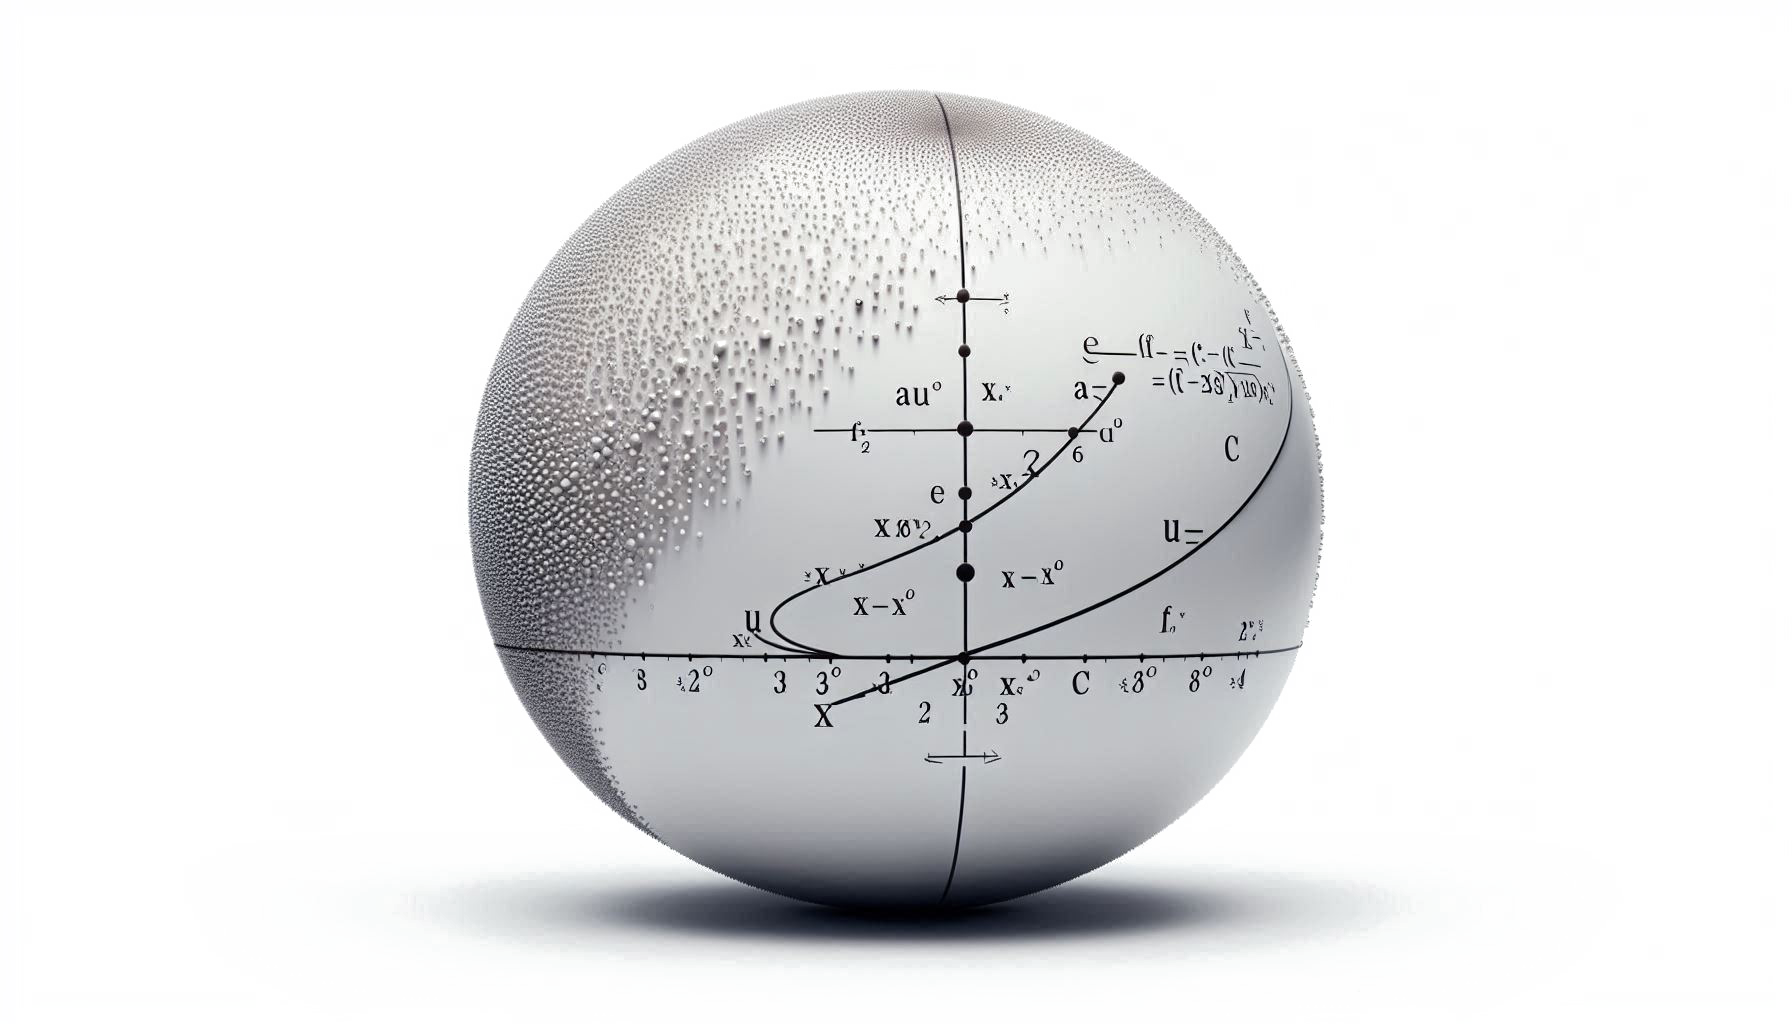
\includegraphics[width=0.6\linewidth]{OIG32.ZNLJ.PNG}
    \caption{%
     \footnotesize\textit{View of a stable spherical structure. A dense sphere of nuclei \(\protect\Op{\Psi}_N\). It could represent a compact DUT object, an equilibrium state of the \(\protect\Op{\Psi}_N\) fluid, or the ultra-compact internal structure of the core of a noncommutative black hole.}
    }
    \label{fig:Figura8}
\end{figure}

\subsection{Commutative Limit: Recovery of GR and SM}
\label{subsec:commutative_limit_final}
The vacuum state of DUT "Solution 0" is postulated to be commutative (\( \langle \Op{\Theta}^{\mu\nu} \rangle = 0 \)). In this limit, the effective action derived from the SAP must reduce exactly to the action of General Relativity coupled to the Standard Model, plus the Lagrangian of a massive scalar field \( \mathcal{L}_{\Psi_N} \) (\Cref{eq:L_PsiN_explicit_final_redux}). This recovery must be a **direct and verifiable consequence** of the explicit calculation of the SAP expansion (Phase 2c of the roadmap).

\subsection{Compatibility with Black Hole Thermodynamics}
\label{subsec:black_hole_thermo_final}
Any theory of quantum gravity must be able to explain the microscopic origin of the Bekenstein-Hawking entropy \( S_{\text{BH}} = A / (4 L_{\text{Pl}}^2) \). In DUT, it is hypothesized that the relevant microstates (\( \mathcal{N} \)) are related to the quantum degrees of freedom of the nuclei \( \Op{\Psi}_N \) and the *dynamic* NC geometric structure generated near the horizon of a black hole (where \( \Op{\Theta} \) could be significantly non-zero, even if the distant vacuum is commutative). A major challenge is to:
\begin{itemize}
    \item Identify and count these microstates \( \mathcal{N} \) within the DUT framework.
    \item Calculate the statistical entropy \( S_{\text{stat}} = k_B \ln \mathcal{N} \).
    \item Demonstrate that \( S_{\text{stat}} \) reproduces the Bekenstein-Hawking formula in the appropriate limit, including possible corrections due to the dynamic NCG (see \Cref{sec:paradoja_informacion_final}).
\end{itemize}
This requires a deep understanding of the quantum description of \( \Op{\Psi}_N \) and the emergent NC geometry.

\section{Connections to Fundamental Problems}
\label{sec:fundamental_problems_final}

We explore how DUT, within the "Solution 0" framework, conceptually addresses some key problems in fundamental physics.

\begin{figure}[htbp]
    \centering
    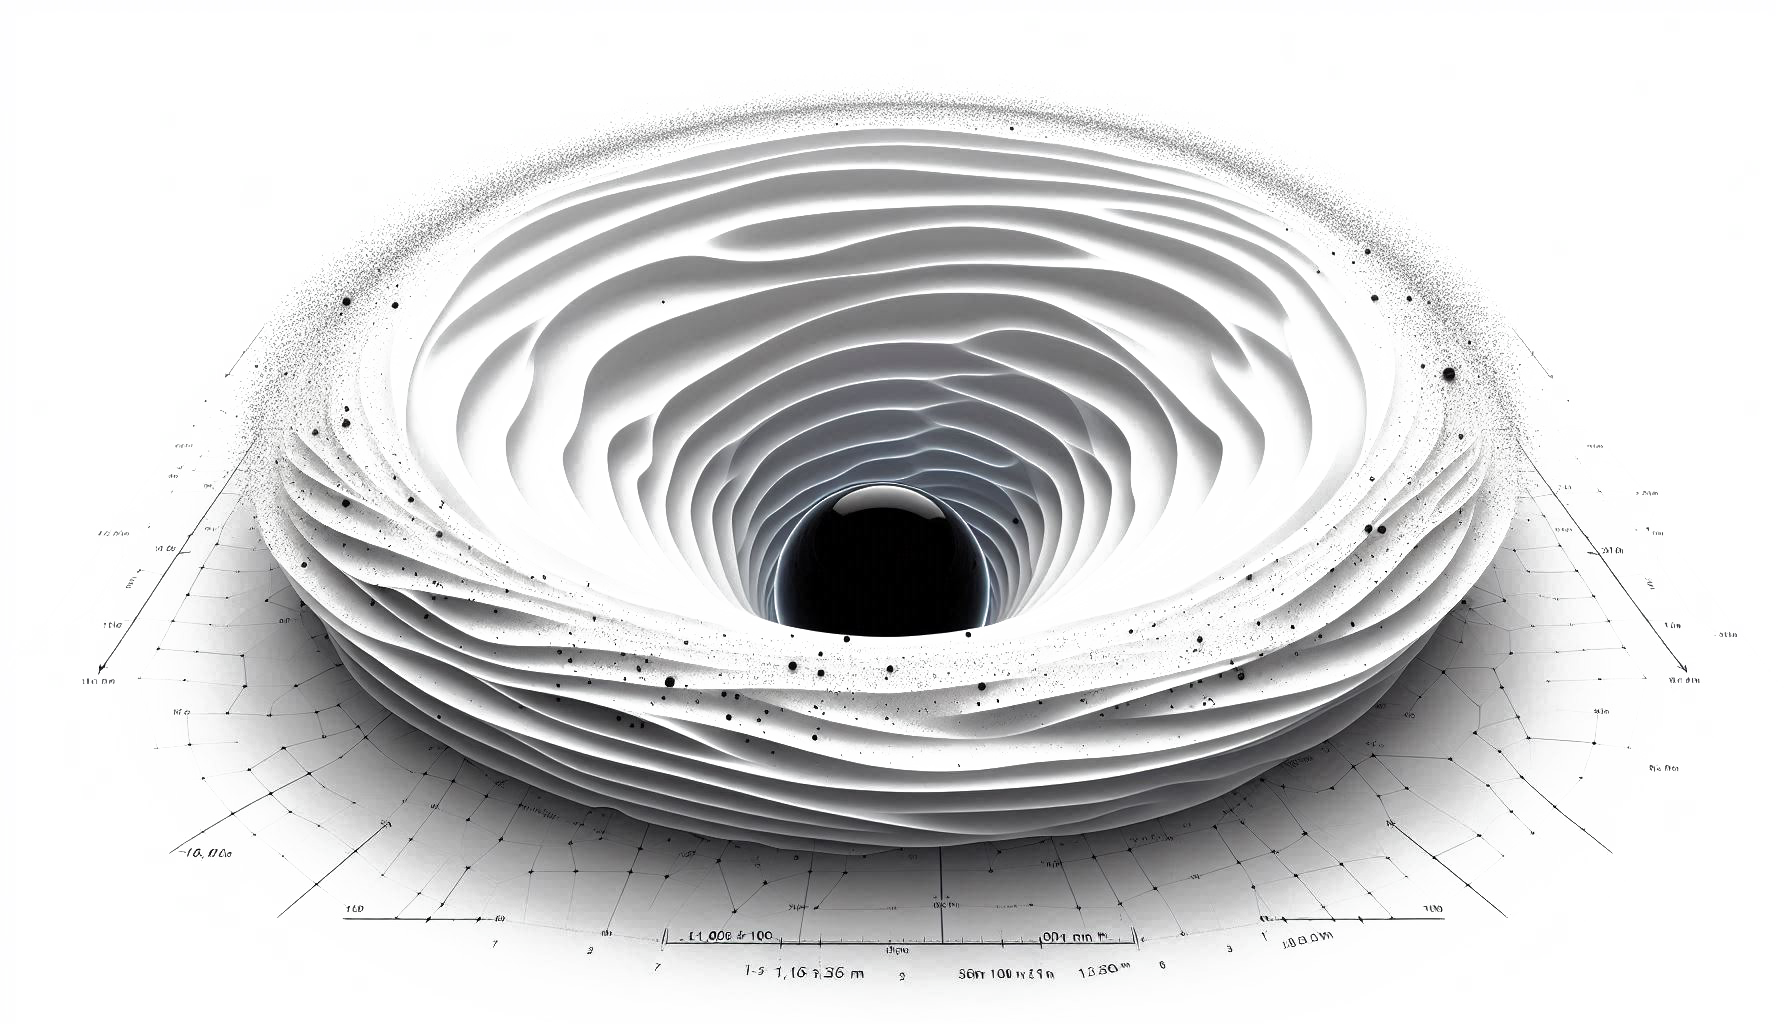
\includegraphics[width=0.6\linewidth]{OIG27.ZNLJ.PNG}
    \caption{%
     \footnotesize\textit{Configuration with a central dark core, surrounded by a diffuse halo hosting dark substructures in symmetric distribution. The background shows scattered particles and radial lines. Could be interpreted in DUT as a DUT topological defect (vortex, monopole) with satellite structures, or a bound system of \(\protect\Op{\Psi}_N\) condensates.}
    }
    \label{fig:Figura9}
\end{figure}

\subsection{The Hierarchy Problem}
\label{sec:problema_jerarquia_final}
The hierarchy problem refers to the large discrepancy between the electroweak scale (\( \sim \SI{100}{GeV} \)) and the Planck scale (\( \Mpl \sim \SI{1e19}{GeV} \)), and why the Higgs mass (\( m_H \)) is so small compared to \( \Mpl \), despite quantum corrections that should drive it to \( \sim \Mpl \).
\textbf{DUT Conceptual Proposal:} The dynamic NCG \( \Op{\Theta}(\Op{\Psi}_N) \), activated at high energies (near \( \Lambda \sim \Mpl \)) or in the presence of \( \Op{\Psi}_N \) excitations, could act as a **natural regulator** of quantum corrections to the Higgs mass. The idea is that the noncommutative structure modifies propagators and vertices at high energies such that quadratic divergences are smoothed or cancelled.
\textbf{Key Challenges:}
\begin{itemize}
    \item The effectiveness of this regularization crucially depends on the **specific magnitude and form** of \( \Op{\Theta}(\Op{\Psi}_N) \) derived from the SAP.
    \item The **UV/IR mixing** problem (\Cref{ssubsec:renormalization_final}), which could reintroduce problematic sensitivities to the NC scale, must be overcome.
    \item An **explicit calculation** of radiative corrections to \( m_H^2 \) within DUT's dynamic NC QFT framework is required to verify if the regularization is sufficient.
\end{itemize}
Therefore, solving the hierarchy problem is **not automatic** in DUT and depends on the detailed quantum structure of the theory (Phase 3b of the roadmap).

\subsection{The Cosmological Constant Problem ('Solution 0')}
\label{sec:problema_cc_final_revised}
This problem has two aspects: (1) Why is the vacuum energy predicted by QFT (\( \rho_{\text{vac}}^{\text{QFT}} \sim \Mpl^4 \)) \( \sim 10^{120} \) times larger than the observed value? (2) What is the nature of the observed dark energy density (\( \rho_{DE} \)) causing the current accelerated expansion? \citep{Weinberg1989CosmoConst}.
DUT "Solution 0" addresses this as follows:

\paragraph{1. Cancellation of QFT Vacuum (\( \rho_{\text{vac}}^{\text{QFT}} \)).}
The central proposal is the **hypothesis of cancellation via supertrace** (\Cref{hyp:cc_cancel_final}). It is postulated that the fundamental action is calculated via \( S = \Str_{\mathcal{H}}(f(D_{\text{DUT}}^2/\Lambda^2)) \). If the total Hilbert space \( \mathcal{H} \) decomposes into bosonic and fermionic sectors \( \mathcal{H} = \mathcal{H}_B \oplus \mathcal{H}_F \) with equal dimensionality (or a more general spectral structure with cancellation), the supertrace can annihilate the constant term of the heat kernel expansion:
\[
a_0 \propto \Str_{\mathcal{H}}(\mathbb{I}) = \Tr_{\mathcal{H}_B}(\mathbb{I}) - \Tr_{\mathcal{H}_F}(\mathbb{I}) \approx 0.
\]
This would cancel the main contribution (\(\sim \Lambda^4\)) to the cosmological constant. Although DUT does not assume explicit supersymmetry, the structure of the operator \( D_{\text{DUT}} \) and the space \( \mathcal{H} \) must be designed to implement this spectral cancellation \citep{ChamseddineConnes1997}.
\textbf{Critique:} This is a **very strong and unproven hypothesis**. It requires a specific symmetry structure in \( D_{\text{DUT}} \) and an **explicit calculation of \( \Str_{\mathcal{H}} \)** to verify it (Phase 2b of the roadmap).
\begin{equation} \label{eq:cancelacion_vacio_str_final_redux}
 \rho_{\text{vac}}^{\text{bare}} \propto \Lambda^4 a_0 \propto \Lambda^4 \Str_{\mathcal{H}}(\mathbb{I}) \approx 0.
\end{equation}

\paragraph{2. Observed Dark Energy (\( \rho_{DE} \)).}
Since \( \Op{\Psi}_N \) emerges as massive (\( m_N \sim \Lambda \)) in "Solution 0", it **cannot be the quintessence** explaining \( \rho_{DE} \). The possibilities within base DUT are limited:
\begin{itemize}
    \item **Cancellation Residue:** The supertrace cancellation might not be perfect, leaving a small residue: \( \Str_{\mathcal{H}}(\mathbb{I}) = \delta \neq 0 \). In this case, \( \rho_{DE} \sim \delta \Lambda^4 \). Explaining the observed value would require \( \delta \sim 10^{-122} \). Can such a tiny value arise naturally from the \( \Str_{\mathcal{H}} \) calculation? This is highly speculative.
    \begin{equation}\label{eq:residuo_vacio_final_redux}
    \rho_{\text{vac}}^{\text{eff}} \sim (\text{Residual } \Str) \Lambda^4.
    \end{equation}
    \item **New Physics:** If \( \Str_{\mathcal{H}} = 0 \) exactly or the residue is incorrect, the observed DE would require physics beyond the DUT "Solution 0" framework (e.g., an extension of the SAP, other light fields not considered).
\end{itemize}
It should be noted that the explanation via a constant residue (\(w=-1\)) would be in tension with observational hints (though not conclusive) suggesting a possible dynamic nature of dark energy (\(w(z) \neq -1\)) \citep[see e.g., analysis in][]{DESI:2024mwx, Abdalla:2022}. Confirming dynamic DE would likely require extensions to the DUT-S0 framework.
In summary, "Solution 0" links the solution to the main CC problem to the hypothesis \( \Str_{\mathcal{H}} \approx 0 \), but leaves the explanation of the observed DE as an additional challenge or an indication of the need to go beyond the minimal framework.

\subsection{The Cosmological Tensions (H0 / S8)}
\label{sec:tensiones_cosmo}
The standard $\Lambda$CDM cosmological model currently faces significant tensions between measurements of the current expansion rate \(H_0\) and the amplitude of matter clustering \(S_8\) inferred from the early universe (mainly CMB) and those obtained from late-universe probes \citep[e.g.,][]{Abdalla:2022}. It is important to note that the base DUT "Solution 0" framework, focused on fundamental unification and CC cancellation via \(\Str_{\mathcal{H}} \approx 0\), **does not offer an intrinsic and direct solution to these tensions**. While modifications to the expansion history or structure growth could emerge from the full SAP calculation (still pending), specifically addressing these tensions might require extensions to the minimal DUT framework or physical mechanisms (such as interactions in the dark sector or early dark energy) that are not part of the base postulates of "Solution 0". Resolving these tensions remains an open challenge for modern cosmology.

\section{Quantum Mechanics of Spacetime Nuclei (\texorpdfstring{\(\protect\Op{\Psi}_N\)}{PsiN})}
\label{sec:mecanica_cuantica_psi_n_final}

The quantum nature of the nuclei \( \Op{\Psi}_N \) (massive in "Solution 0"), their transition to classical behavior, and the connection to the information paradox are discussed.

\begin{figure}[htbp]
    \centering
    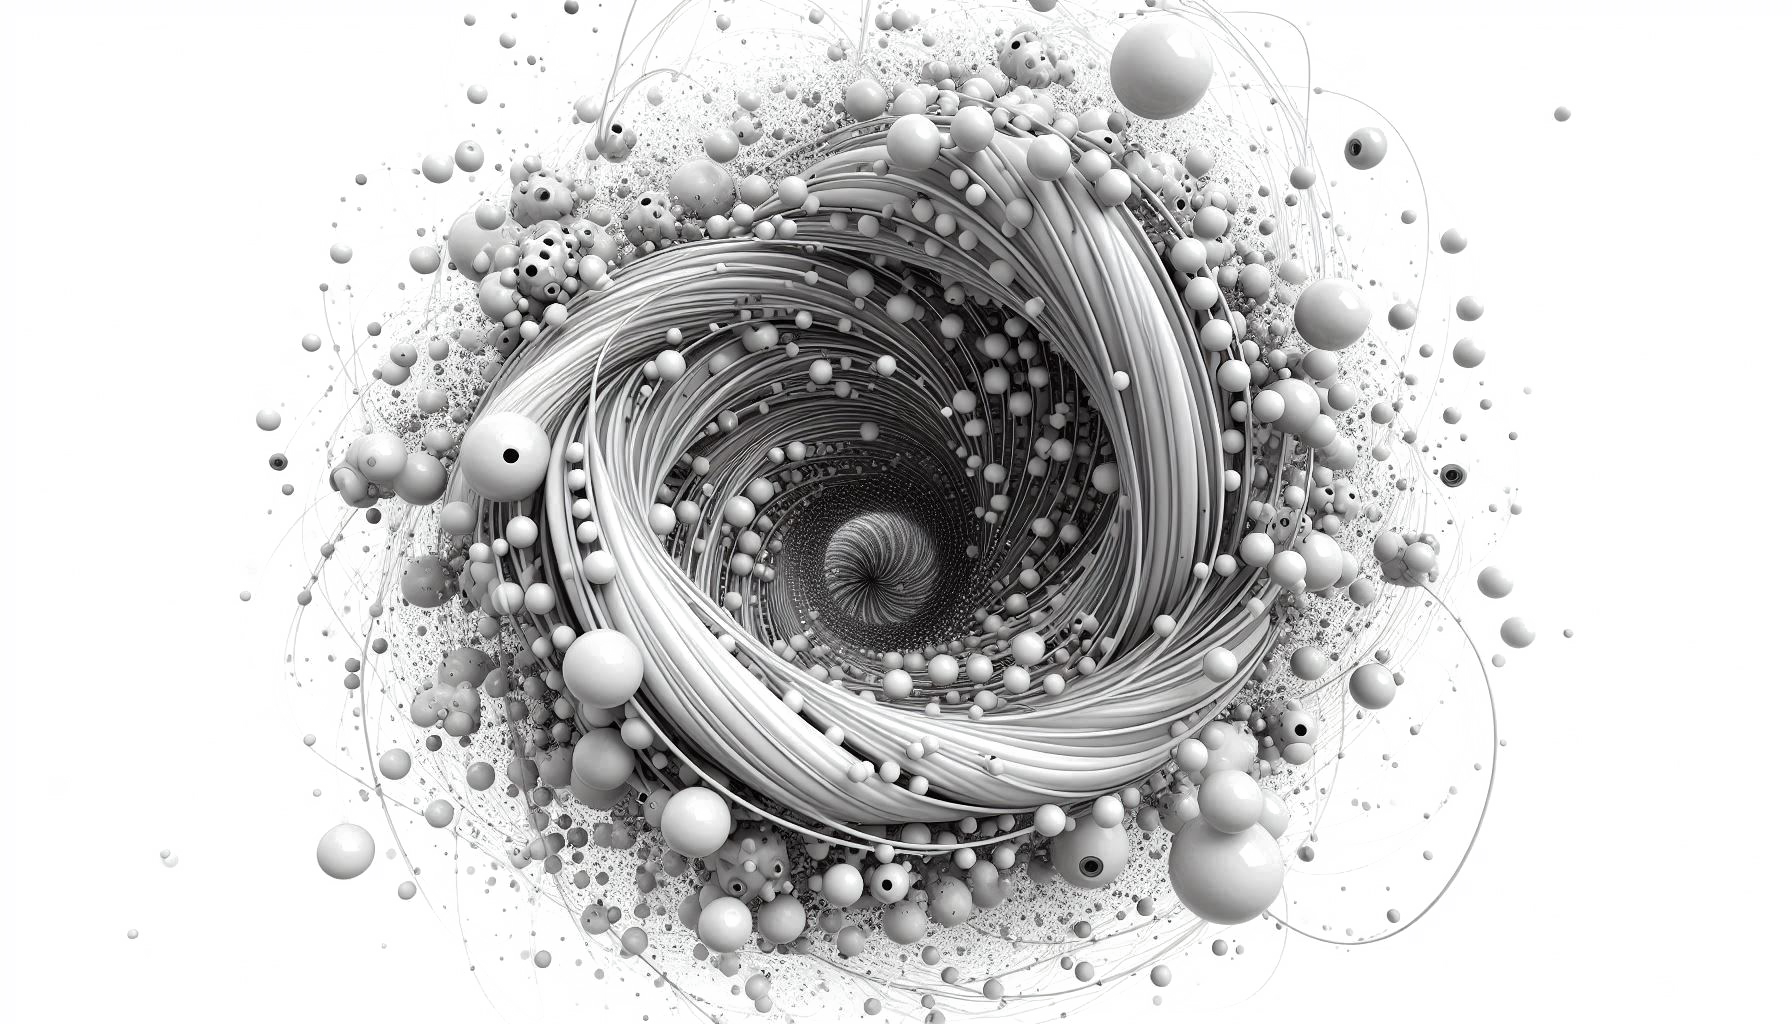
\includegraphics[width=0.6\linewidth]{OIG15.ZNLJ.PNG}
    \caption{%
        \footnotesize\textit{Spherical volume densely populated by nuclei \(\protect\Op{\Psi}_N\) with diverse properties, featuring a central light source. Illustrates a collective state of the \(\protect\Op{\Psi}_N\) medium, possibly in an excited state or showing the propagation of a wave or other collective excitation from the center, as would be described in DUT.}
    }
    \label{fig:Figura10}
\end{figure}


\subsection{Primordial Quantum State and Decoherence}
\label{sec:decoherence_final}
A primordial quantum state of the universe, \(|\Psi_0\rangle\), is postulated, possibly involving a superposition of \( \Op{\Psi}_N \) configurations and NC geometry (analogous to proposals like the Hartle-Hawking wave function of the universe \citep{HartleHawking1983WFU}). The emergence of the classical universe (with smooth geometry and commutative vacuum) is attributed to the process of quantum **decoherence** \citep{ZurekDecoherenceReview, JoosZehDecoherenceBook, KieferQuantumGravityBook}. The interaction of fundamental degrees of freedom (\( \Op{\Psi}_N \), NC geometry) with matter fields (acting as the "environment") would induce the loss of quantum coherence on macroscopic scales. This process would select a "pointer basis" of classically stable states \citep{ZurekPointerBasis, Kiefer:2008sw}, which in DUT "Solution 0" must correspond to those where \( \Op{\Psi}_N \) is near its minimum and, therefore, \( \langle \Op{\Theta} \rangle \approx 0 \).
**Challenge:** Explicitly modeling this decoherence process within the DUT context is a **major theoretical challenge**.

\subsection{Proposed Resolution of the BH Information Paradox}
\label{sec:paradoja_informacion_final}

The information paradox \citep{KieferQuantumGravityBook} arises from the apparent loss of quantum unitarity during black hole (BH) evaporation via Hawking radiation. DUT proposes a conceptual resolution based on dynamic NCG:
\begin{enumerate}
    \item \textit{Singularity Regularization:} Dynamic NCG (with \( \Op{\Theta} \neq 0 \) generated near \( r=0 \)) is expected to prevent the formation of a classical point singularity \citep[cf.][]{Nicolini:2008aj}, modifying the internal structure of the BH.
    \item \textit{Nonlocal Information Storage:} It is speculated that information falling into the BH is not destroyed but encoded nonlocally in the **noncommutative correlations** between the \( \Op{\Psi}_N \) degrees of freedom and the NC geometry in the region where \( \Op{\Theta} \neq 0 \). The precise encoding and retrieval mechanism needs to be detailed.
    \item \textit{Retrieval via Correlations}:** The emitted radiation (analogous to Hawking) would not be perfectly thermal but would contain **subtle correlations** (derived from the underlying NC structure) that carry the information out during evaporation, preserving unitarity.
    \item \textit{Corrected Entropy}:** The BH entropy would receive corrections due to NC degrees of freedom. Formula \eqref{eq:entropia_corregida_final_redux} is a schematic ansatz:
        \begin{equation} \label{eq:entropia_corregida_final_redux}
        S_{\text{BH}}^{\text{DUT}} = \frac{A}{4 L_{\text{Pl}}^2} + \gamma f(\Op{\Theta}_{\text{horizon}}) + \dots
        \end{equation}
        where the correction term \( f(\Op{\Theta}) \) would depend on the magnitude of the noncommutativity dynamically generated near the horizon. This requires **rigorous derivation** from counting \( \Op{\Psi}_N \) microstates in DUT (\Cref{subsec:black_hole_thermo_final}).
\end{enumerate}
This proposal is conceptual and needs **rigorous mathematical development** for validation and concrete predictions about correlations in the radiation.

\section{Cosmological Origin and Emergence of Time in DUT}
\label{sec:cosmo_origin_final}

Ideas about the origin of the universe and the nature of time in DUT "Solution 0" are explored.

\begin{figure}[htbp]
    \centering
    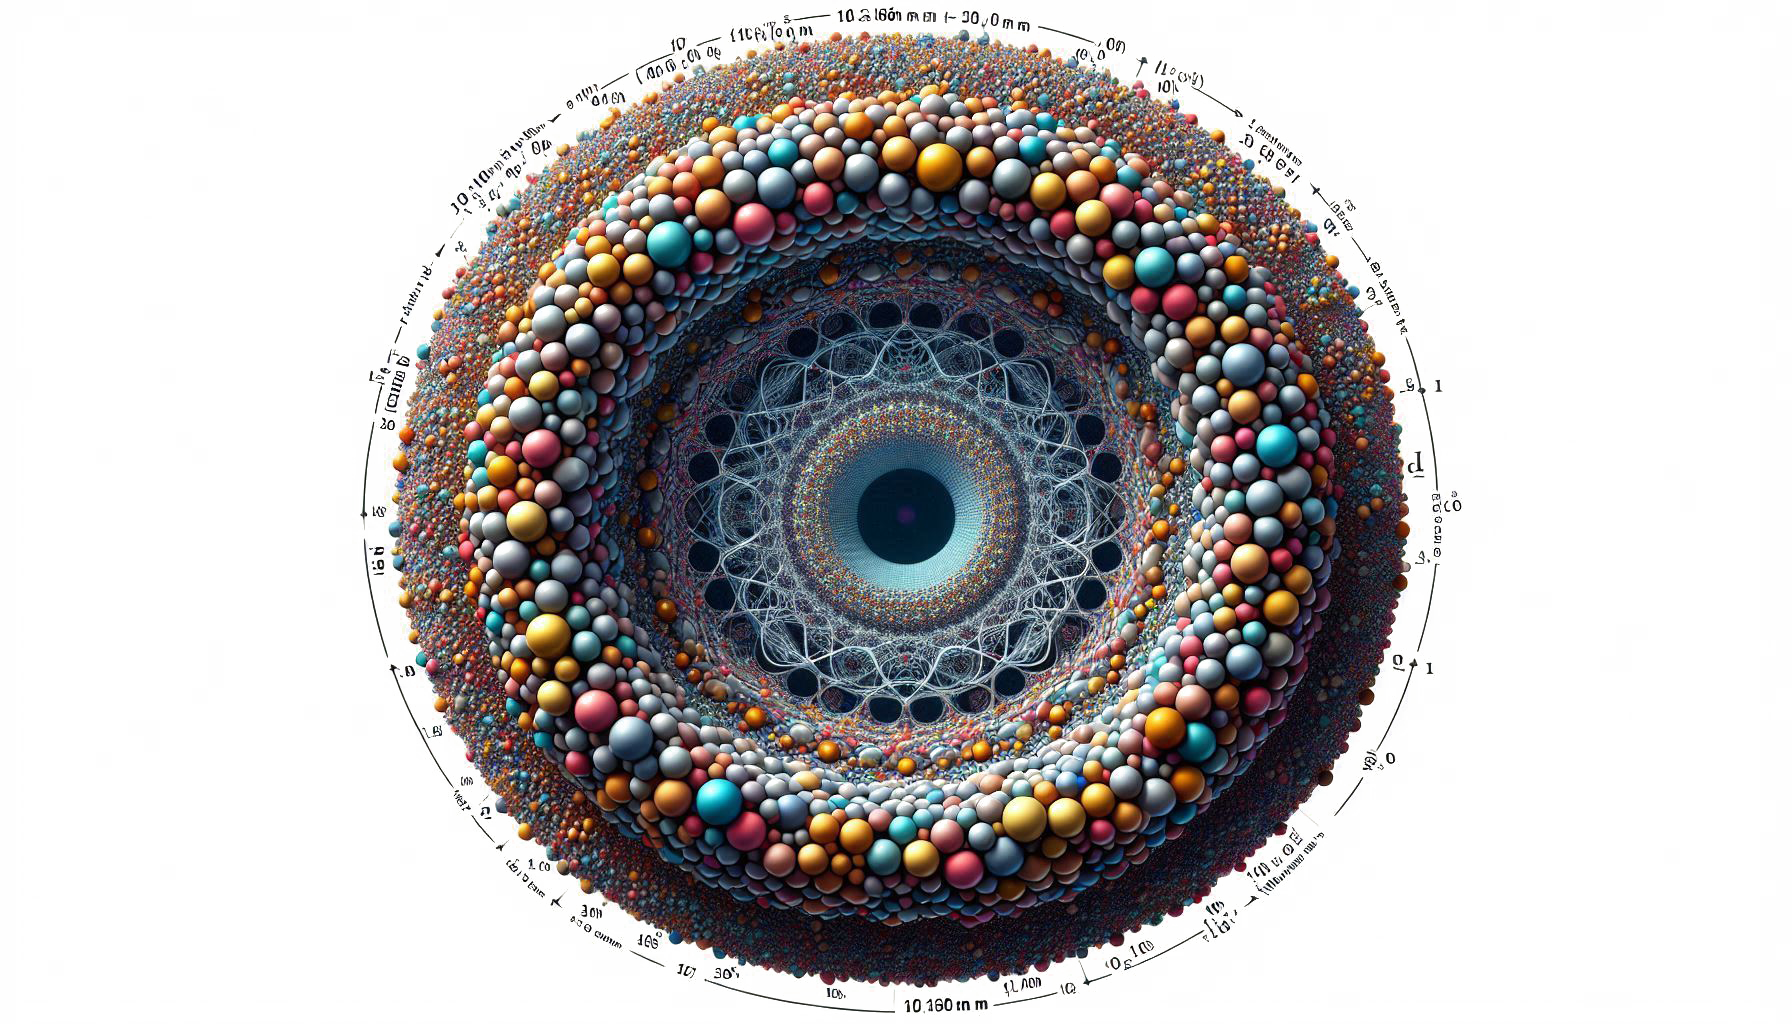
\includegraphics[width=0.6\linewidth]{OIG2.ZNLJ.PNG}
    \caption{%
        \footnotesize\textit{Cross-section of a toroidal structure revealing discrete inner layers formed by nuclei \(\protect\Op{\Psi}_N\). Emphasizes internal organization, suggesting distinct phases, quantum levels, or internal stratification within a compact object or specific region described by DUT.}
    }
    \label{fig:Figura11}
\end{figure}

\subsection{Universe Formation and Cosmic Inflation}
\label{subsec:universe_formation_inflation_final_revised}
It is postulated that the universe emerges from a primordial quantum state \(|\Psi_0\rangle\). A key question is the mechanism of **cosmic inflation** \citep{Guth:1980zm, Linde:1981mu, Albrecht:1982wi, Starobinsky1980} in this framework. Could the \( \Op{\Psi}_N \) field, despite being massive (\( m_N \sim \Lambda \)), have played a role during inflation? This would depend on the complete form of the potential \( V(\Psi_N) \) derived from the SAP. Mechanisms like massive field inflation, hybrid inflation (if \( \Psi_N \) couples to another inflaton field), or inflation driven by higher-curvature terms generated in the SAP expansion (\( a_4 \)) might be possible.
Regardless of the mechanism, DUT must be able to:
\begin{itemize}
    \item Calculate predictions for primordial cosmological observables: scalar spectral index \( n_s \), tensor-to-scalar ratio \( r \), and level of non-Gaussianity \( f_{NL} \) \citep{Maldacena2003NonGaussian}.
    \item Consistently incorporate the effects of dynamic NCG (\( \Op{\Theta} \)) during inflation \citep[cf.][]{Aschieri2022}.
    \item Compare these predictions with precision observations of the CMB and LSS \citep{Planck2018Inflation, Planck2018NonGaussianity, BICEP:2021xfz}.
\end{itemize}
Performing these **detailed calculations is a pending and crucial task** (part of Phase 4 of the roadmap).

\subsection{Initial State of the Discrete Nuclei}
\label{subsec:initial_state_nuclei_final}
The model postulates the nuclei \( \hat{\Psi}_N \) as pre-existing fundamental entities. The state \( |\Psi_0\rangle \) represents their primordial configuration. The ultimate origin of these nuclei and the nature of \( |\Psi_0\rangle \) are beyond the current scope of the theory, being questions of a more speculative nature.

\subsection{Emergence of Time}
\label{subsec:time_emergence_final}
The "problem of time" in quantum gravity \citep{ProblemOfTimeRef} refers to the difficulty of defining a well-defined time evolution in a context where spacetime itself is dynamic and quantum. How does the flow of time we experience emerge? DUT, like other QG theories, must address this question. Possible approaches include:
\begin{itemize}
    \item **Relational Time:** Defining time emergently through the relation between different physical degrees of freedom (using one as a "clock" to measure the evolution of others). With massive \( \Psi_N \), it cannot be the main cosmological clock.
    \item **Thermodynamic Time:** Relating the "arrow of time" to the increase of some form of entropy, possibly associated with the \( \Op{\Psi}_N \) degrees of freedom or decoherence \citep{KieferQuantumGravityBook, Kiefer:2008sw}.
\end{itemize}
This is a **deep conceptual challenge** for DUT.

\subsection{Limitations and Open Questions (Cosmological Origin)}
\label{subsec:origin_limitations_final_revised}
The DUT "Solution 0" framework faces significant open questions regarding cosmological origin:
\begin{itemize}
    \item Can dynamic NCG avoid the initial Big Bang singularity \citep[cf.][]{Nicolini:2008aj}?
    \item What physics determines the initial state \( |\Psi_0\rangle \)?
    \item Can DUT (with massive \( \Psi_N \)) provide an inflation mechanism compatible with observations?
    \item Does it offer a coherent solution to the problem of time?
    \item What is the ultimate nature of the nuclei \( \hat{\Psi}_N \)? Are they truly fundamental or do they emerge from something deeper?
\end{itemize}

\section{Proposed Cosmological Solutions ('Solution 0')}
\label{sec:cosmological_solutions_final_revised}

This section summarizes DUT "Solution 0" proposals to explain cosmological phenomena such as Dark Matter and early structure formation. The explanation for Dark Energy, as discussed, relies on the CC cancellation hypothesis or requires extensions.

\begin{figure}[htbp]
    \centering
    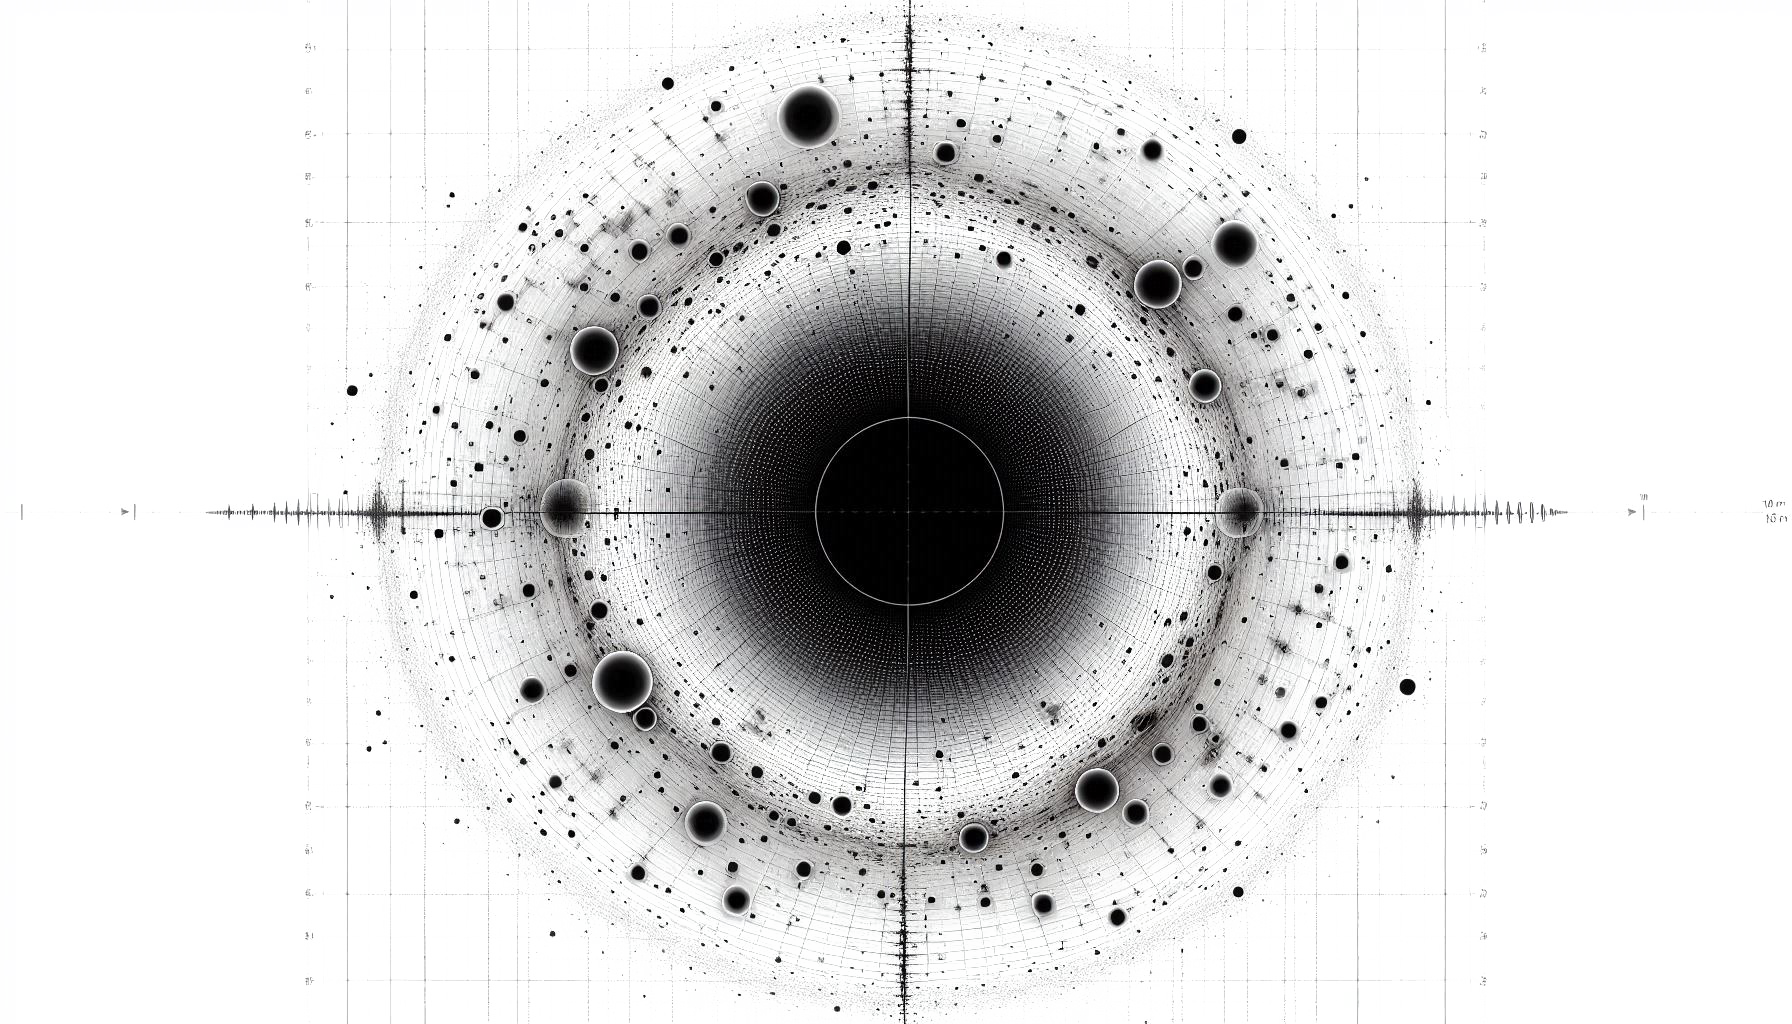
\includegraphics[width=0.6\linewidth]{OIG34.ZNLJ.PNG}
    \caption{%
       \footnotesize\textit{Configuration dominated by a central dark core, surrounded by a diffuse halo with several associated dark substructures. Faint radial lines and a background of scattered dots complete the image. Within DUT, it could visualize a DUT black hole seed or a complex topological defect interacting with its \(\protect\Op{\Psi}_N\) environment.}
    }
    \label{fig:Figura12}
\end{figure}

\subsection{Dark Energy and CC Problem ('Solution 0')}
\label{subsec:dark_energy_final_revised}

\subsubsection{Cancellation of QFT Vacuum (\texorpdfstring{$\Str_{\mathcal{H}} \approx 0$}{Str=0})}
\label{sec:cancelacion_vacio_final_revised}
The central proposal (\Cref{sec:problema_cc_final_revised}) is reiterated: the vast vacuum energy predicted by QFT is cancelled due to a spectral symmetry in \( D_{\text{DUT}} \) resulting in \( \Str_{\mathcal{H}}(...) \approx 0 \) (\Cref{hyp:cc_cancel_final}). The **explicit demonstration of this cancellation is a primary and pending requirement** (Phase 2b of the roadmap).

\subsubsection{Observed Dark Energy: Residue or New Physics?}
\label{sec:observed_dark_energy_revised}
Since the base \( \Op{\Psi}_N \) is massive (\( m_N \sim \Lambda \)), it **cannot be quintessence**. The small observed \( \rho_{DE} \) could be:
\begin{itemize}
    \item A **small residue** from the supertrace cancellation (if \( \Str_{\mathcal{H}}(...) \) is \( \sim 10^{-122} \)).
    \item Or indicative of **new physics** beyond the DUT "Solution 0" framework.
\end{itemize}
Determining which is the case requires the explicit calculation of \( \Str_{\mathcal{H}} \). As mentioned (\Cref{sec:problema_cc_final_revised}), an explanation via a constant residue would be in tension with hints of dynamic DE.

\subsection{Dark Matter Candidates in DUT (with Heavy \texorpdfstring{$\Psi_N$}{PsiN})}
\label{subsec:dark_matter_final_revised}

In a context where traditional dark matter candidates like WIMPs face increasingly severe experimental constraints from direct detection experiments \citep[see summary in][]{PDG2022}, DUT "Solution 0" proposes the following alternative candidates, whose viability depends on the detailed structure derived from the SAP:

\subsubsection{Emergent Noncommutative Axions}
\label{sec:axiones_nc_final_revised}
Light pseudoscalar fields (axion-like, \( \mathcal{A} \)) could arise from the internal structure of the SAP or extensions. Their effective Lagrangian would include NC terms (\( \star \)) dependent on \( \Op{\Theta}(\Op{\Psi}_N) \), as in \eqref{eq:L_axion_nc_final_redux}.
\begin{equation} \label{eq:L_axion_nc_final_redux}
\mathcal{L}_{\text{axion}} \approx \frac{1}{2} (\partial \mathcal{A})^2 - V_{PQ}(\mathcal{A}) + \text{NC Couplings}(\mathcal{A}, \Op{\Psi}_N, \Op{\Theta}, G, F).
\end{equation}
Their properties (mass \( m_{\mathcal{A}} \), decay constant \( f_a \), couplings, relic abundance) must be **calculated from the complete SAP**. They could behave as cold or fuzzy DM (ULDM/FDM). Experimental tests include direct (haloscopes, helioscopes) and indirect searches \citep{PDG2022, PerezGarcia2024}. %Marsh:2022 is another good general ref on axions

\subsubsection{Topological Dark Matter (Defects of Heavy \texorpdfstring{$\Psi_N$}{PsiN})}
\label{sec:dm_topologica_final_revised}
If the potential \( V(\Psi_N) \) derived from the SAP for the massive field \( \Psi_N \) (with \( m_N \sim \Lambda \)) featured degenerate minima (due to higher-order terms or couplings), **topological defects** (domain walls, cosmic strings, monopoles) could form during phase transitions in the very early universe (possibly at the end of inflation or later). If these defects were stable (or sufficiently long-lived) and produced with the correct energy density \eqref{eq:defect_density_final_redux}, they could constitute DM (likely cold, given the expected mass \( \sim \Lambda \)).
\begin{equation} \label{eq:defect_density_final_redux}
n_{\text{top}} \sim (\xi L)^{-3} \quad \text{or} \quad n_{\text{top}} \sim H_{\text{trans}}^3 e^{-S}.
\end{equation}
**Requirements:** 1) Derive the complete \( V(\Psi_N) \) from the SAP. 2) Analyze if it admits degenerate minima and stable defects. 3) Calculate the relic abundance of these defects. Observational tests include searches for DM annihilation or decay (\(\gamma\), \(\nu\), antimatter \citep{Hooper2017_HAWC, PDG2022}) and effects on large-scale structures.

\subsection{Early Formation of Supermassive Black Holes (SMBHs)}
\label{subsec:smbh_formation_final_revised}

The existence of massive SMBHs at high redshift \(z > 6\), confirmed and detailed by recent JWST observations \citep[e.g.,][]{Labbe:2023}, challenges models of growth by accretion from stellar seeds. An alternative is primordial seeds, such as Primordial Black Holes (PBHs) \citep{CarrHawking1974PBH}.
**DUT Proposal:** Quantum fluctuations of the \( \Op{\Psi}_N \) field (even being massive) during or after inflation, potentially **enhanced by dynamic NCG effects** (\( \Op{\Theta} \neq 0 \) at that epoch), could have been large enough on certain scales to collapse gravitationally and form PBHs. **This mechanism could offer an explanation for the early appearance of the massive SMBHs observed by JWST, generating seeds that are more massive or earlier than standard stellar ones.** The phenomenological form for the enhanced power spectrum of \( \Psi_N \) \eqref{eq:P_PsiN_nc_peak_final_redux} serves as a target to be derived.
\begin{equation} \label{eq:P_PsiN_nc_peak_final_redux}
\mathcal{P}_{\Psi_N}(k) \approx \mathcal{P}_{\Psi_N}^{\text{std}}(k) \left[ 1 + \text{Enhancement}(k; \Psi_N, \Theta_{\text{inflation}}) \right].
\end{equation}
**Required Validation:**
\begin{enumerate}
    \item Calculate \( \mathcal{P}_{\Psi_N}(k) \) consistently from a DUT inflation model (with heavy \( \Psi_N \) and derived dynamic \( \Theta \)).
    \item Calculate the mass function and abundance of the resulting PBHs.
    \item Verify compatibility with the strong existing observational constraints on PBHs across different mass ranges \citep{Carr:2020gox}.
\end{enumerate}
Potential signatures include specific contributions to the stochastic gravitational wave background (GWB), detectable by LISA \citep{LISA:2017, Auclair2023LISA} or PTAs \citep{NANOGrav:2023gor}, depending on the PBH mass.

\section{Proposal of Novel Predictions and Experimental Verification}
\label{sec:novel_predictions_final_revised}

For DUT "Solution 0" to be testable, it must generate unique, falsifiable quantitative predictions derived rigorously from its fundamental framework (SAP, derived dynamic NCG). Key proposals are presented below, emphasizing the need for derivation.

\begin{figure}[htbp]
    \centering
    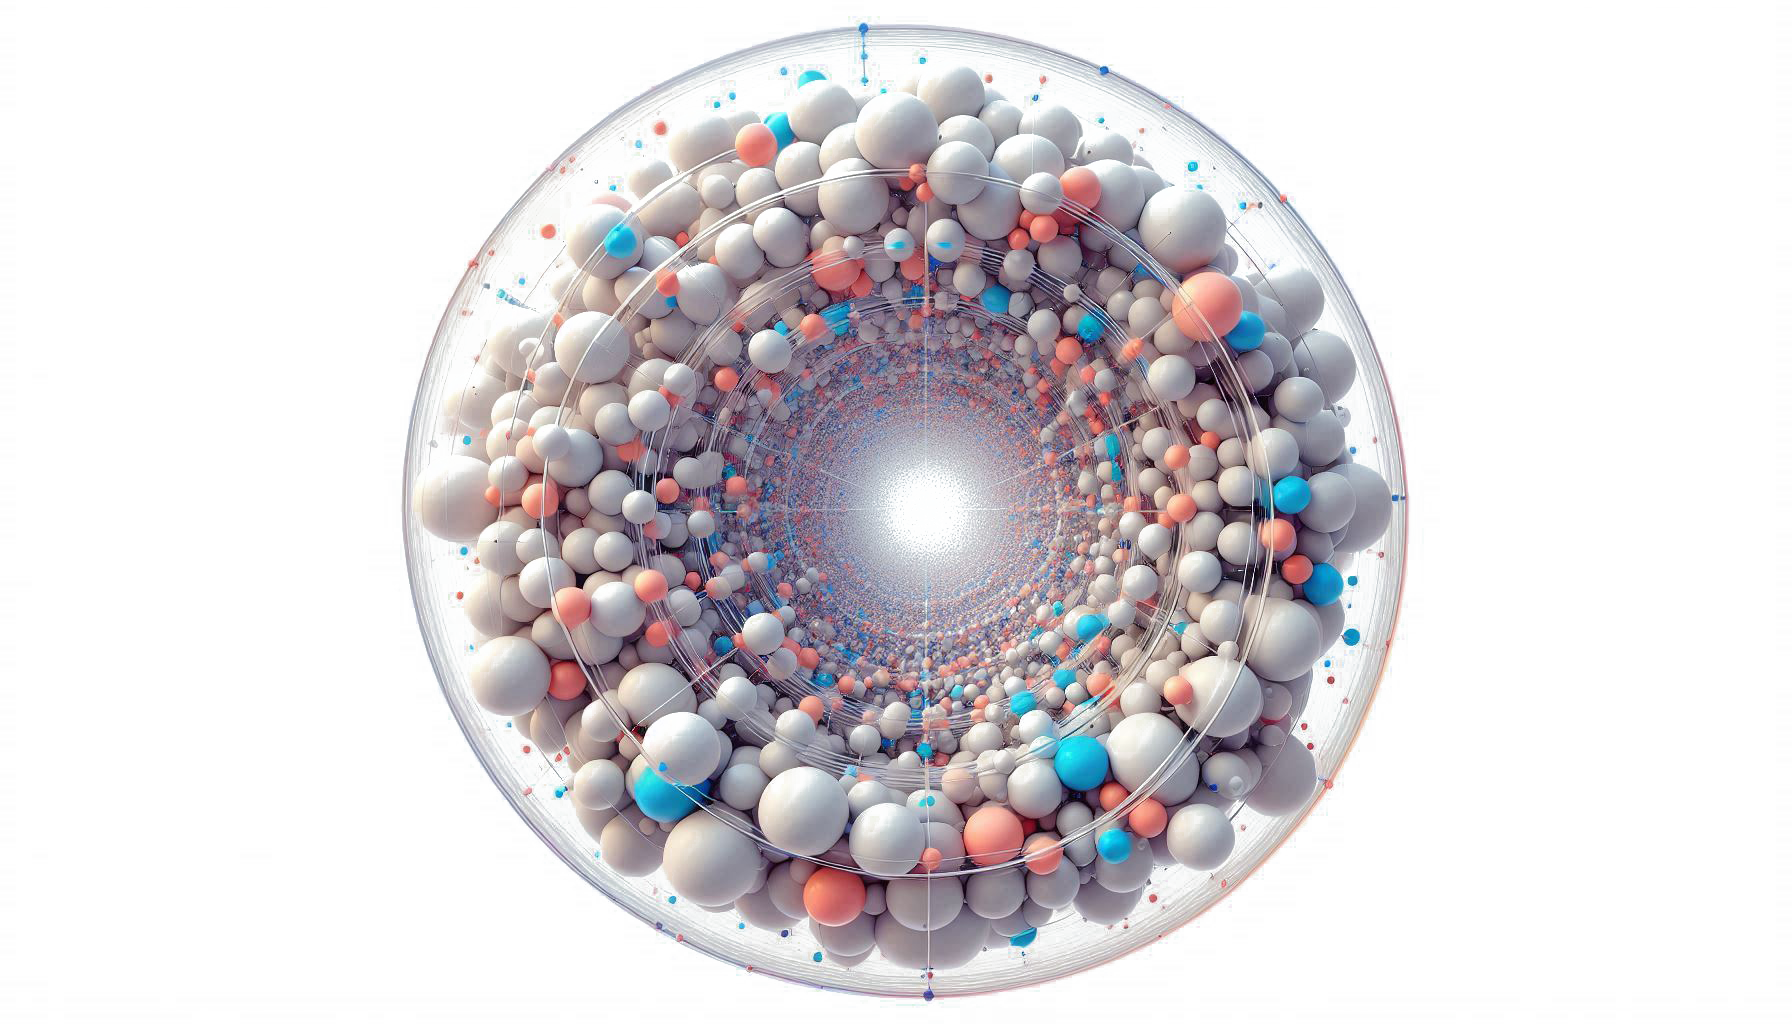
\includegraphics[width=0.6\linewidth]{OIG10.ZNLJ.PNG}
    \caption{%
      \footnotesize\textit{Visualization of waves or excitations emanating spherically from a bright center within a volume populated by nuclei \(\protect\Op{\Psi}_N\). Could represent DUT radiation emission (analogous to Hawking) from a central object, or the propagation of collective modes in the \(\protect\Op{\Psi}_N\) medium.}
    }
    \label{fig:Figura13}
\end{figure}

\subsection{Dynamic Lorentz Invariance Violation (LIV)}
\label{subsec:liv_specific_final_revised}

\textbf{Central Prediction Proposal:}
Given \( \langle \Op{\Theta} \rangle = 0 \) in vacuum, DUT "Solution 0" predicts **absence of LIV for particles propagating in vacuum at low energies**. However, the dynamic NCG \( \Op{\Theta}(\Op{\Psi}_N) \) can induce LIV effects **dependent on the state or environment**:
\begin{itemize}
    \item In regions with **high energy density or curvature** where \( \Op{\Psi}_N \) can be significantly excited (generating \( \Op{\Theta} \neq 0 \)).
    \item For particles with **energies near the fundamental scale** \( \Lambda \sim \Mpl \), where the NC structure becomes intrinsically relevant.
\end{itemize}
The modified dispersion relation (MDR) would take the form \eqref{eq:mdr_tud_redux} only under these conditions:
\begin{equation} \label{eq:mdr_tud_redux}
E^2 \approx p^2c^2 \left[ 1 + \xi \left(\frac{E}{\Lambda_{\text{LIV}}}\right)^n f(\text{environment}) \right].
\end{equation}
Here, \( f(\text{environment}) \) represents the dependence on the local state (\( \propto \langle \Op{\Theta}^2 \rangle \)?), \( \Lambda_{\text{LIV}} \) is expected \( \sim \Mpl \) (to be derived from SAP), \( n \) (1 or 2) must be calculated from the modified propagators, and \( \xi = \pm 1 \).

This prediction is particularly interesting in light of current stringent limits. The absence of LIV in vacuum predicted by DUT-S0 is consistent with the high-precision null results from observatories like LHAASO, MAGIC, H.E.S.S., Fermi-LAT \citep[e.g.,][]{Lang:2019uug, LHAASO_GRB221009A_LIV, HAWC_HESS_LIV, FermiLAT_GRB090510_LIV, PierreAuger:2021tog} based on photon propagation over cosmological distances. DUT-S0 would naturally satisfy these limits without requiring the fundamental scale \( \Lambda_{LIV} \) to be necessarily much larger than \( M_{Pl} \), provided the effect is predominantly linked to \( \Op{\Theta} \neq 0 \). However, the theory predicts the possibility of detectable LIV effects in extreme astrophysical environments or for particles with energies \( E \to \Lambda \sim M_{Pl} \).

\textbf{Key Observational Signature:}
Search for **energy-dependent time delays** in very high-energy astroparticles (gamma rays, neutrinos) from extreme astrophysical sources (GRBs, AGNs) where \( \Op{\Theta} \) could be generated. The **absence of LIV in low-energy or vacuum searches** \citep{KosteleckyDataTables} is consistent with this prediction.

\textbf{Essential Future Work (Phase 4a):}
Rigorously derive the form of \( f(\text{environment}) \), the order \( n \), and confirm \( \Lambda_{\text{LIV}} \sim \Mpl \) from the complete SAP and the consistently derived form of \( \Op{\Theta}(\Op{\Psi}_N) \).

\textbf{Key Experiments:}
LHAASO \citep{LHAASO_GRB221009A_LIV}, **CTA**, HAWC \citep{HAWC_HESS_LIV}, Fermi-LAT \citep{FermiLAT_GRB090510_LIV}, IceCube, Auger \citep{PierreAuger:2021tog}.

\subsection{Specific Signatures in the Matter Power Spectrum}
\label{subsec:power_spectrum_final_revised}

\textbf{Prediction Proposal:}
Primordial quantum fluctuations of heavy \( \Op{\Psi}_N \) and/or effects of dynamic NCG \( \Op{\Theta} \) during inflation could leave specific imprints on the statistics of cosmological perturbations, modifying the power spectrum \(P(k)\) and generating primordial non-Gaussianities \( f_{NL} \). The form \eqref{eq:pk_tud_redux} is a placeholder to be determined.
\begin{equation} \label{eq:pk_tud_redux}
P_{\text{DUT}}(k) = P_{\Lambda\text{CDM}}(k) \times \left[ 1 + \Delta P(k; \Psi_N, \Theta_{\text{inflation}}) \right].
\end{equation}

\textbf{Distinctive Signatures:}
\begin{itemize}
    \item Characteristic modifications (oscillations, steps, peaks) in \(P(k)\) dependent on the inflationary dynamics of \( \Psi_N/\Theta \). If PBHs form, a peak at small scales would be expected.
    \item Generation of primordial non-Gaussianity (\( f_{NL} \)) with a specific shape (local, equilateral, orthogonal, etc.) linked to the \( \Psi_N/\Theta \) interaction vertices during inflation.
\end{itemize}

\textbf{Essential Future Work (Phase 4b):}
Develop a self-consistent inflation model within DUT (incorporating heavy \( \Psi_N \) and derived dynamic \( \Op{\Theta} \)) and explicitly calculate the corrections \( \Delta P(k) \) and the shape and amplitude of \( f_{NL} \).

\textbf{Key Experiments:}
Precision CMB observations (Planck \citep{Planck2018Inflation, Planck2018NonGaussianity}, future like CMB-S4), large-scale structure (LSS) surveys (Euclid \citep{EuclidCollaboration}, DESI, LSST/Vera C. Rubin Observatory, SKA), Lyman-\(\alpha\) forest.

\subsection{Dark Matter Density Profiles (If DM = \texorpdfstring{$\Psi_N$}{PsiN} Defects)}
\label{subsec:dm_profile_final_revised}

\textbf{Prediction Proposal:}
If Dark Matter consists of stable topological defects derived from the potential \( V(\Psi_N) \) (heavy) obtained from the SAP (\Cref{sec:dm_topologica_final_revised}), their self-interaction properties (possibly null or very small) and early formation could lead to specific predictions about DM halo structure:
\begin{itemize}
    \item **Central Density Profile:** Could differ from the cuspy profiles (NFW-type) predicted by standard WIMP simulations, or from the cored profiles associated with self-interacting or fuzzy DM models. The exact shape (\( \rho(r) \)) must be determined.
    \item **Subhalo Distribution:** The abundance and mass function of subhalos might differ from \(\Lambda\)CDM predictions.
\end{itemize}
The form \( \rho \propto r^{-\gamma} \) \eqref{eq:rho_dm_tud_redux} is purely speculative.
\begin{equation} \label{eq:rho_dm_tud_redux}
\rho_{\text{DUT-defect}}(r) = \text{Profile Derived from Specific Simulations}.
\end{equation}

\textbf{Essential Future Work (Phase 4b):}
Requires completing Phases 1-2 of the roadmap to obtain \( V(\Psi_N) \), analyzing the existence and properties of stable defects, and then performing **cosmological N-body simulations** incorporating the specific properties of these defects as DM particles.

\textbf{Testing Method:}
Detailed observations of galaxy rotation curves (especially dwarfs), analysis of strong and weak gravitational lensing, studies of galaxy cluster dynamics (Data from Hubble, JWST, Euclid, LSST/Vera C. Rubin Observatory, etc.).

\subsection{High-Frequency Gravitational Wave Background (GWB)}
\label{subsec:gwb_high_freq_final_revised}

\textbf{Prediction Proposal:}
Possible **first-order phase transitions** in the very early universe, associated with the dynamics of \( \Op{\Psi}_N \) or other fields present in the DUT SAP, could generate a stochastic gravitational wave background (GWB) \citep{Witten:1984rs, Hogan:1986qda}. If the transition occurs at an energy scale \( T_* \) near \( \Lambda \sim \Mpl \), the resulting GWB peak frequency, redshifted to today, could lie in the **high-frequency region (MHz-GHz or higher)**, a window currently poorly explored experimentally. The spectral shape \( \Omega_{\text{GW}}(f) \) \eqref{eq:gwb_hf_tud_redux} would depend on the transition parameters (strength \( \alpha \), duration \( \beta^{-1} \), bubble wall velocity \( v_w \)).
\begin{equation} \label{eq:gwb_hf_tud_redux}
\Omega_{\text{GW}}(f)h^2 = \text{Calculated Spectrum from DUT Phase Transition}.
\end{equation}

\textbf{Essential Future Work (Phase 4b):}
1) Identify possible first-order phase transitions from the effective potential \( V(\Psi_N, H, ...) \) derived from the complete SAP and its thermal evolution. 2) Calculate the transition parameters (\( \alpha, \beta, T_*, v_w \)). 3) Calculate the resulting spectrum \( \Omega_{\text{GW}}(f)h^2 \).

\textbf{Key Experiments:}
Development of future **high-frequency GW detectors** (based on resonant cavities, electromagnetic detectors, etc.). If PBH formation (\Cref{subsec:smbh_formation_final_revised}) generates a secondary GWB, it might be detectable by LISA or PTAs.

\subsection{Summary and Validation Strategy}
\label{subsec:summary_validation_predictions_revised}
These predictions (dynamic LIV, signatures in \(P(k)/f_{NL}\), DM halo structure, GWB) represent examples of potentially unique signatures of DUT "Solution 0". Their validation and utility for testing the theory critically depend on being able to **derive them quantitatively** from the fundamental framework once the consistency and calculation challenges described in the roadmap (\Cref{subsec:quantitative_roadmap_detailed}) are resolved, particularly Phases 1-3. Phase 4 would be dedicated to these phenomenological calculations.
Future observational tests with instruments like LISA, Einstein Telescope, CMB-S4, Euclid, Vera C. Rubin Observatory, CTA, and future EHT upgrades will be crucial to confront these quantitative predictions once made.

\section{Preliminary Discussion and Comparison with Other Theories}
\label{sec:comparison_final}

DUT ("Solution 0", with detailed challenges and strategies) is placed in the context of other approaches towards quantum gravity and unification.

\begin{table}[htbp]
\centering
{
\footnotesize
\begin{tabularx}{\textwidth}{@{}l X X X X X@{}} % Column spec okay (l XXXXX)
\toprule
\textbf{Aspect} & \textbf{DUT} & \textbf{String/M-Theory} & \textbf{LQG} & \textbf{Asymptotic Safety (AS)} & \textbf{CDT} \\
\midrule
Dimensions        & 4D fund. (\( \Psi_N \) emerges) & 10D/11D \citep{BFSS1997, IKKT1997} & 4D & 4D & 4D emergent \\ \addlinespace
Singularities     & Avoided by dynamic NCG? (prop., \Cref{sec:collapse_TUD_ME}) & Resolved (some) & Resolved \citep{Ashtekar:2006wn} & Could be resolved \citep{Bonanno:2017pkg} & Avoided (simul.) \citep{Ambjorn:2005qt} \\ \addlinespace
Unification        & Grav+SM (via NCG/SAP-\(\Str\)) \citep{ConnesChamseddine1997} & Grav+Gauge & Grav. quantum & Grav+SM (UV?) \citep{Eichhorn:2018yfc} & Grav. quantum \\ \addlinespace
Dark Matter     & NC Axions / Defects of heavy \( \Psi_N \) (prop.) & Axions, WIMPs (landscape) & No prediction & No prediction & No prediction \\ \addlinespace
Dark Energy/$\Lambda$ & \textbf{Cancel. \( \rho_{\text{vac}} \) (via \( \Str_\mathcal{H} \approx 0 \)? Key hyp.). DE = CC Residue (w=-1)? or Extension. \textit{Tension w/ hints w(z)\(\neq\)-1}.} (\(\Psi_N\) base massive is NOT DE).
& Paisaje \citep{Bousso:2000xa} & QLC \citep{Ashtekar:2009mb}    & RG origin? \citep{Bonanno:2001xi} & Phase trans.? \citep{Ambjorn:2008wc} \\ \addlinespace
H0/S8 Tensions   & \textbf{Not resolved in base TUD.}
& Alleviated by landscape/mods? & Not intrinsically resolved & Could be addressed? & Not intrinsically resolved \\ \addlinespace
Specific Predic. & LIV **dynamic** (\( \Lambda \sim \Mpl \)), Early SMBH seeds?, \(P(k)/f_{NL}\) modif.?, DM Profile?, GWB(HF)? (\textbf{Derivation Pending})
& SUSY, Extra Dim. & Geom. spectrum, LIV \citep{Barrau:2017tcd} & UV fixed points? & Spectral dim. \citep{Ambjorn:2005db} \\ \addlinespace
Mathematical Status & Conceptual (\textbf{Rigor of dynamic NCG (Jacobi), Full SAP-\(\Str\) derivation, Stability pending}, \textbf{Detailed Strategies Proposed})
& High/Complex & Medium \citep{RovelliLQG} & Medium (FRG) \citep{Reuter:2012id}    & Medium (Simul.) \citep{Loll:2019rdj} \\ \addlinespace
Main Problem & \textbf{Prove math consistency \& perform full SAP-\(\Str\) derivation. Calculate \( \Str_{\mathcal{H}} \). Stability. Quantitative Calculations.} (Execute roadmap \Cref{subsec:quantitative_roadmap_detailed}) % CORRECTED '&' to '\&'
& Experiment, Non-perturb., Landscape & Dynamics, Classical limit, Matter coupling  & Fixed point existence, Truncations & Continuum limit, Matter \\ \addlinespace
Verifiability    & Potential \textbf{if} theoretical challenges overcome \& calculations performed (Predictions \Cref{sec:novel_predictions_final_revised}). % CORRECTED '&' to '\&'
& Very Difficult & Very Difficult & Indirect? & Difficult \\
\bottomrule
\end{tabularx} % Correct closing command
}
\caption{Schematic comparison of DUT ("Solution 0" Detailed and Updated) with other approaches.}
\label{tab:comparison_revised}
\end{table}

\textbf{Discussion ('Solution 0' Detailed and Updated):}
DUT "Solution 0" presents itself as a unifying framework based on emergent dynamic NCG (commutative vacuum) and the SAP with supertrace. Its focus on 4D is direct. It proposes specific candidates for DM (NC axions, defects of heavy \( \Psi_N \)) whose viability depends on derivation from the SAP. It addresses the main CC problem by postulating cancellation via \( \Str_{\mathcal{H}} \approx 0 \) (requires explicit calculation); observed DE remains a separate issue for the base model (constant residue? extension needed?), especially given hints of dynamic DE. Similarly, **the base framework offers no intrinsic solution to the H0/S8 tensions**. Nonetheless, DUT-S0 generates potentially distinctive predictions relevant to current observations: the possibility of explaining **early SMBH seed** formation (connecting to JWST) and a **dynamic LIV** (consistent with current HE limits but testable). The developmental stage is conceptual, but **detailed strategies** have been outlined to address the crucial mathematical and computational challenges (Jacobi, SAP-\(\Str\) derivation, stability). Its viability depends on the successful execution of the proposed roadmap (\Cref{subsec:quantitative_roadmap_detailed}). Compared to Strings (extra dimensions, landscape) or LQG (difficulty coupling matter, classical limit), DUT offers a different perspective but faces its own formidable challenges of consistency and calculation. Unlike MOG models that modify GR directly on cosmological scales, DUT aims to recover GR as a limit, with deviations linked to the dynamic activation of \( \Op{\Theta} \).


% --- FIGURE 14 ---
\begin{figure}[htbp]
    \centering
    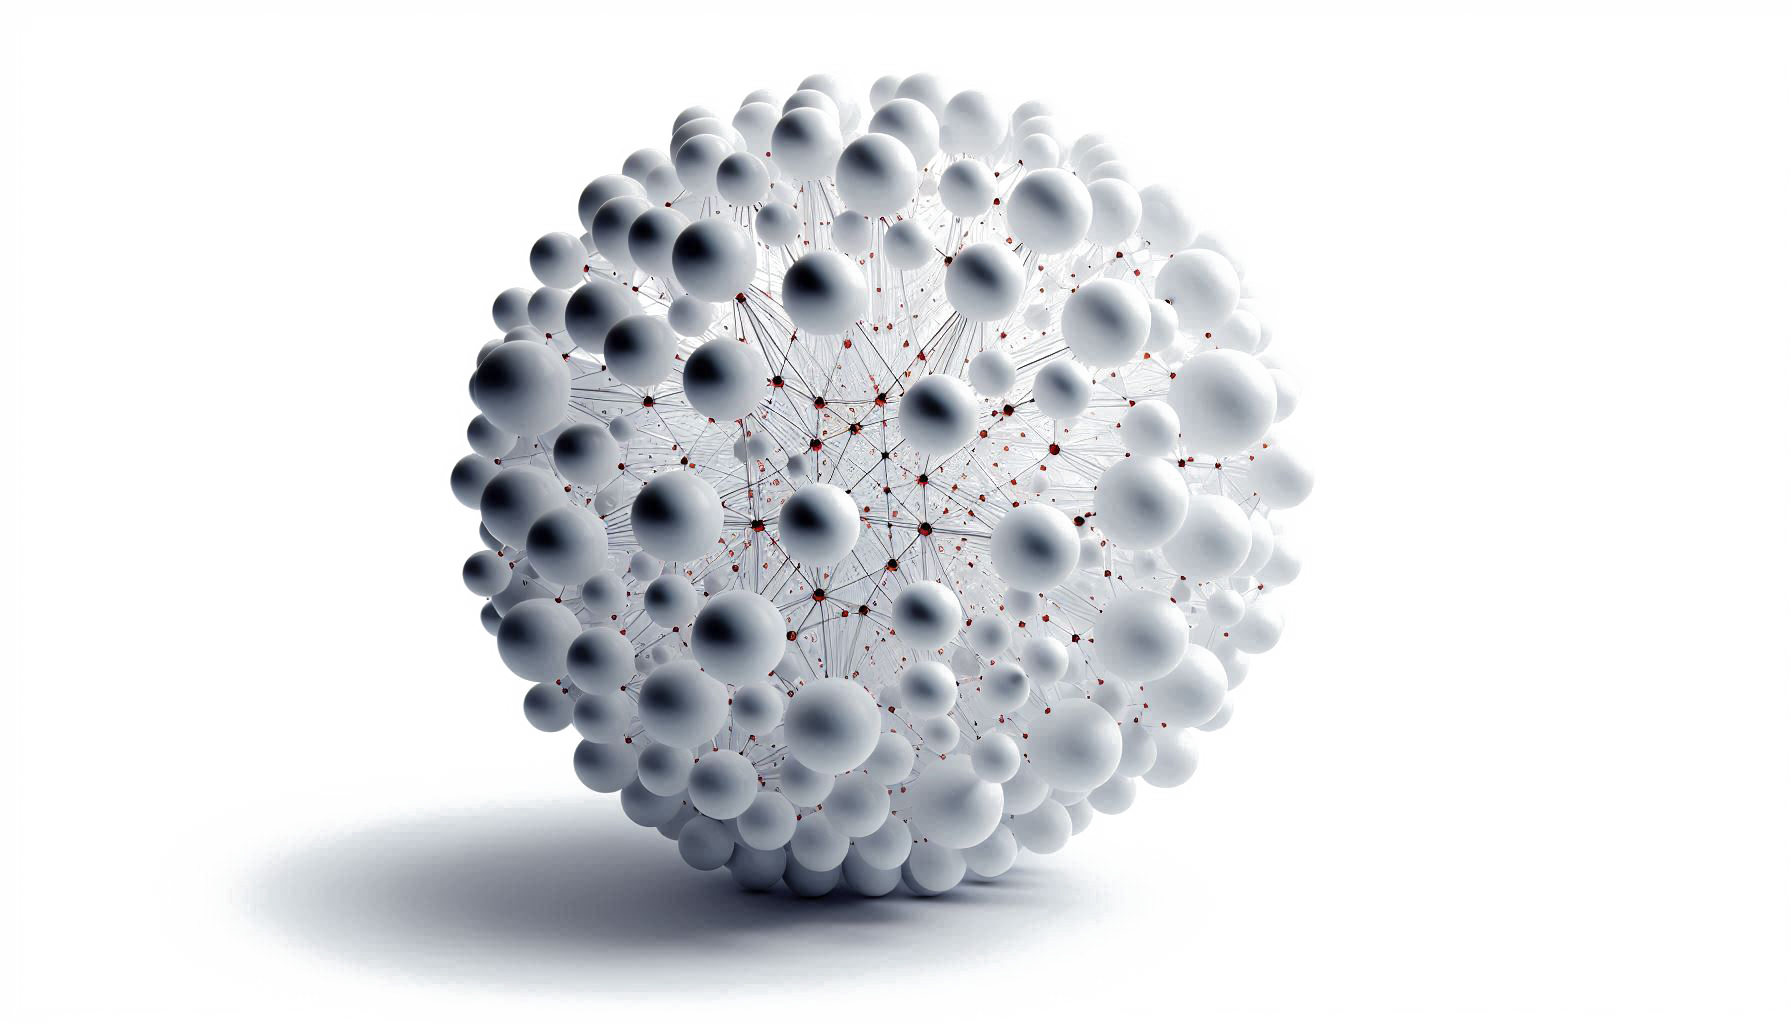
\includegraphics[width=0.6\linewidth]{OIG12.ZNLJ.PNG} % Ensure image exists
    \caption{%
      \footnotesize\textit{Highly ordered structure composed of well-defined, bright concentric rings with a luminous central core. Individual nuclei \(\protect\Op{\Psi}_N\) are distributed on the annular surfaces. Suggests a stable, stratified quantum configuration, perhaps a quantum state of a DUT object with discrete energy levels.}
    }
    \label{fig:Figura14}
\end{figure}

\section{Gravitational Collapse with Standard Model Fields in DUT ('Solution 0')}
\label{sec:collapse_TUD_ME}

The study of gravitational collapse represents a crucial scenario for testing the limits of General Relativity and exploring the effects of quantum gravity. Within the framework of the Discrete Unification Theory (DUT) "Solution 0", the noncommutative (NC) nature of spacetime is a **dynamic and emergent** phenomenon, described by \( \Op{\Theta}^{\mu\nu}(\Op{\Psi}_N) \), which is null in the vacuum (\( \langle \Op{\Theta} \rangle = 0 \)) and activates only when the (massive) field \( \Op{\Psi}_N \) is significantly excited. This introduces potential modifications to the collapse dynamics compared to classical GR, particularly in high-density/curvature regimes.

\begin{figure}[htbp]
    \centering
    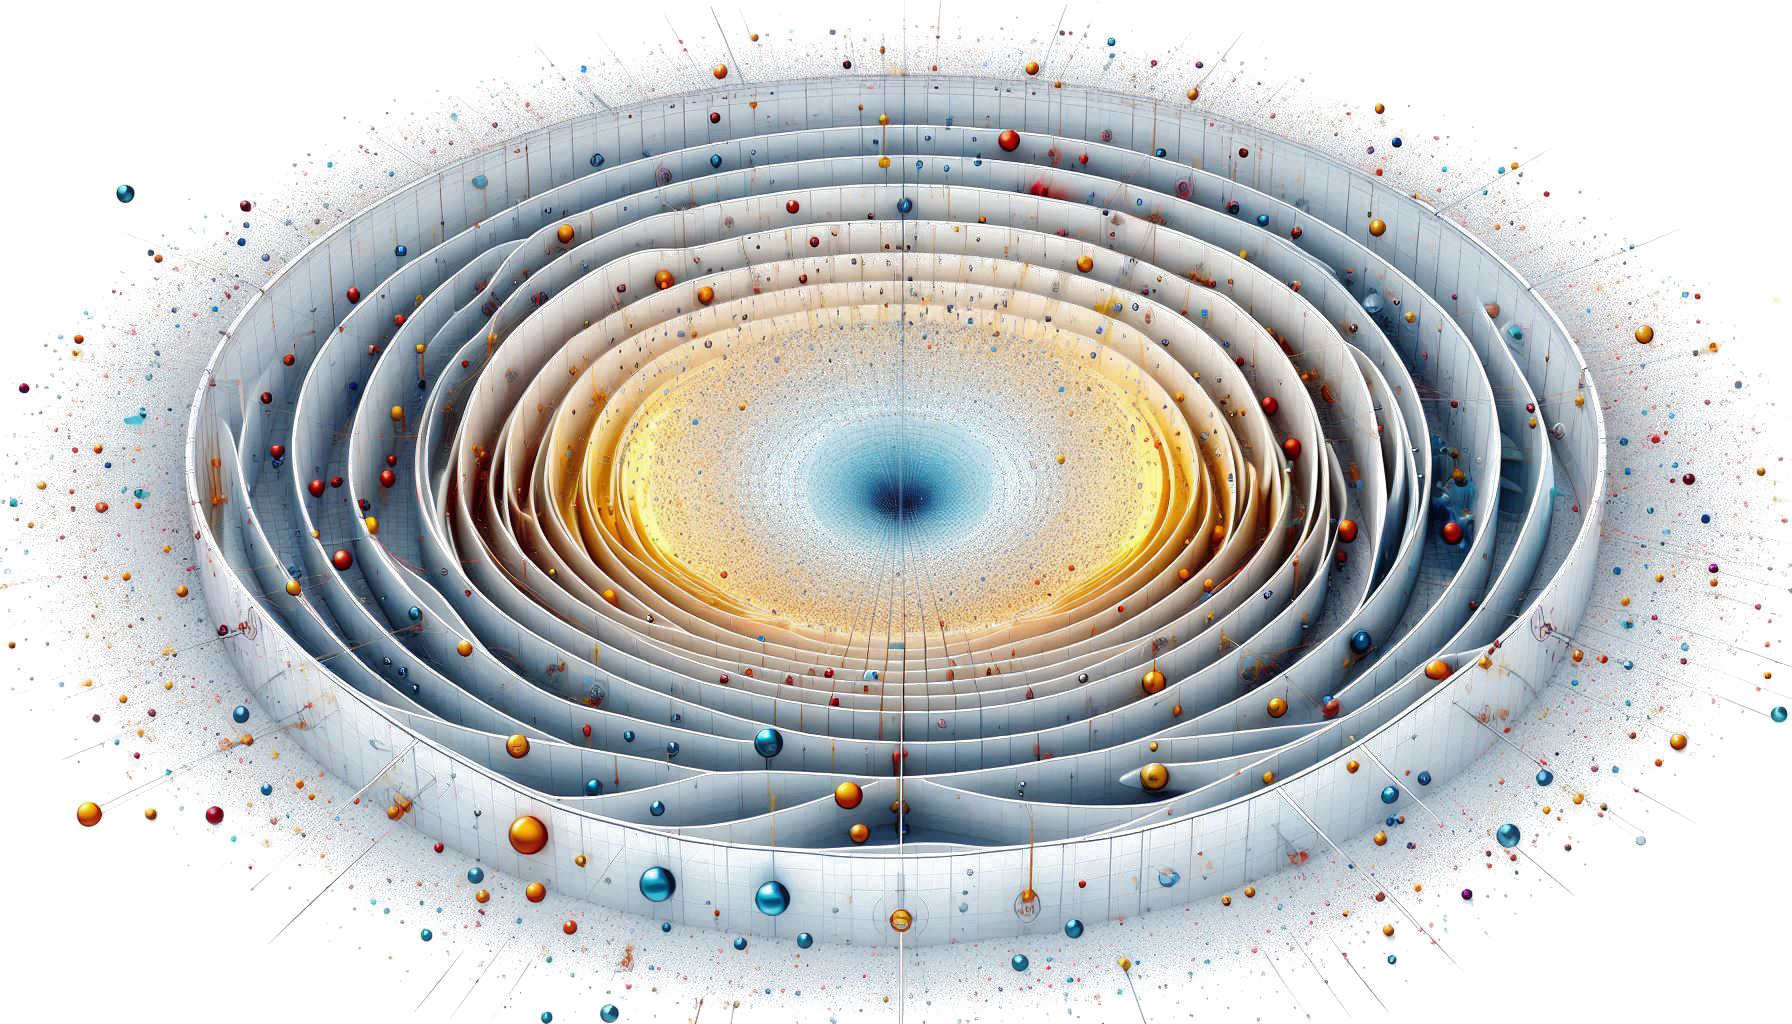
\includegraphics[width=0.6\linewidth]{OIG26.ZNLJ.PNG}
    \caption{%
      \footnotesize\textit{Stratified arrangement of concentric rings with a bright core, populated by discrete nuclei \(\protect\Op{\Psi}_N\). Reinforces the idea of ordered, possibly quantized, internal structures that can emerge from the collective dynamics of \(\protect\Op{\Psi}_N\) in DUT.}
    }
    \label{fig:Figura16}
\end{figure}

\subsection{Theoretical Framework: Coupling and Emergent NC Dynamics}
\label{subsec:collapse_theory}

The SAP (\Cref{post:action_final}) couples SM fields to the dynamic NC geometry \((\Op{g}_{\mu\nu}, \Op{\Theta}(\Op{\Psi}_N))\). Noncommutativity, mediated by \( \Op{\Theta} \) (whose form must be derived from the SAP), only manifests when \( \Op{\Psi}_N \) is excited above its vacuum state.

\subsubsection{Standard Model Fields in Emergent Dynamic NCG}
\label{ssubsec:sm_coupling_nc}

SM fields (fermions \(\psi\), gauge \(A_\mu\), Higgs \(H\)) interact via the \( \star \) product (\Cref{eq:moyal_product_explicit_final}). This product **only differs from the ordinary commutative product in regions where \( \Op{\Theta}(\Op{\Psi}_N) \neq 0 \)**. The resulting modifications to the equations of motion are therefore concentrated in the phases or zones of collapse with sufficient energy density or curvature to excite \( \Op{\Psi}_N \).

\paragraph{Fermions (quarks, leptons):} Their dynamics follow the NC Dirac equation \( ( i\gamma^\mu \mathcal{D}_\mu - m ) \star \psi = 0 \), where \( \mathcal{D}_\mu = \nabla_\mu - i g A^a_\mu T^a \star \). The \( \star \) terms introduce effective nonlocal corrections (dependent on \( \Theta^{\rho\sigma} \) and momenta) to propagation and to the contribution to the energy-momentum tensor \( \hat{T}_{\mu\nu}^{\text{ferm}} \), but only where \( \Theta \neq 0 \).

\paragraph{Gauge fields (photons, gluons, W/Z bosons):} They are described by the NC Yang-Mills action \( \mathcal{L}_{\text{YM-NC}} = -\frac{1}{4} \Tr( \hat{G}^a_{\mu\nu} \star \hat{G}^{a\mu\nu} ) \), with \( \hat{G}^a_{\mu\nu} = \partial_\mu A^a_\nu - \partial_\nu A^a_\mu + g f^{abc} A^b_\mu \star A^c_\nu \). Nonlocal self-interactions and modifications to standard interactions induced by \( \star \) are only relevant where \( \Theta \neq 0 \).

\paragraph{Higgs Field (\( \Phi \)):} The effective potential \( V(\Phi) \star = \lambda ( \Phi^\dagger \star \Phi - v^2 ) \star ( \Phi^\dagger \star \Phi - v^2 ) \) generates additional interaction terms dependent on \( \Theta \) and derivatives of \( \Phi \). These could modify electroweak stability or the scalar's dynamics during the most extreme phases of collapse. (Note: The exact form of the potential must be derived from the SAP).

\subsubsection{Dynamic and Structural Modifications in Collapse}
\label{ssubsec:dynamic_mods_collapse}

The collapse dynamics may differ from classical GR **if and where \( \Op{\Theta} \) activates dynamically**:

\paragraph{Effective energy-momentum tensor (\( \hat{T}_{\mu\nu}^{\text{total}} \)):} Includes the contribution from the massive field \( \hat{T}_{\mu\nu}^{\Psi_N} \) and that of the SM fields modified by \( \star \), \( \hat{T}_{\mu\nu}^{\text{SM-NC}} \). The NC terms in \( \hat{T}_{\mu\nu}^{\text{SM-NC}} \) can generate effective anisotropic pressures (\( P_{\text{NC}} \sim \Theta^2 \dots \)) that counteract collapse in central regions.

\paragraph{Modified Field Equations:} The Einstein-Grau equations (\Cref{eq:einstein_grau_op_final}), \( \Op{G}_{\mu\nu}[g, \hat{\Theta}] = 8\pi G_{\text{eff}} \Op{T}_{\mu\nu}^{\text{total}} \), receive \( \mathcal{O}(\Op{\Theta}) \) corrections (via \( \star \) and explicit dependence) on both sides. These corrections, active only where \( \Op{\Theta} \neq 0 \), are the proposed mechanism for **regularizing the central singularity**, acting as an effective "quantum pressure" or modifying geometry at scales where \( \Op{\Theta} \) is significant.

\paragraph{Effects on Horizon Formation:} Event horizon formation may be affected if a significant \( \Op{\Theta} \) is generated over an extended region *before* the formation of the classical apparent horizon. NC pressures could reduce the effective gravitating mass \( M_{\text{eff}} \approx M - \Delta M_{\text{NC}} \), resulting in a potentially smaller or delayed final horizon radius \( r_H \approx 2 G M_{\text{eff}} \).

\subsubsection{Stability and Causality}
\label{ssubsec:stability_causality_collapse}
The DUT "Solution 0" framework is expected to be Hamiltonially stable, being based on second-order Lagrangians (see detailed analysis in \Cref{subsec:hamiltonian_stability_analysis_detailed}), thus avoiding Ostrogradsky instabilities \citep{OstrogradskiRef, Woodard:2014wia}. Macroscopic causality (\( v_g \le c \)) must be preserved; potential Lorentz Invariance Violations (\Cref{subsec:liv_specific_final_revised}) would be suppressed by \( \Lambda \sim \Mpl \) and activate only dynamically in the presence of \( \Op{\Theta} \).

\subsection{Numerical Methodology for Emergent Dynamic NC Simulations}
\label{subsec:collapse_numerics}

Numerical simulations are crucial for studying the *dynamic* generation of \( \Op{\Theta} \) from commutative initial conditions and evaluating its actual effects on collapse.

\subsubsection{Discretization and Integration Scheme}
\label{ssubsec:discretization_scheme}
Advanced numerical methods like Adaptive Mesh Refinement (AMR) are required to resolve different spatial scales. The \( \star \) product must be implemented numerically, calculating \( \Op{\Theta}^{\mu\nu}_i \) in each cell \( i \) from the local values of the field \( \Op{\Psi}_N \) and its numerical derivatives (\(\Op{\Theta}^{\mu\nu}_i \approx 0\) if \((\Op{\Psi}_N)_i \approx 0\)). A 3+1 formulation (ADM or BSSN type \citep{HenneauxTeitelboim1992}) adapted to the NC Einstein-Grau equations and the dynamics of the massive \( \Op{\Psi}_N \) field is needed. Stable and adaptive time integration schemes (e.g., Runge-Kutta, Leapfrog) respecting the CFL condition must be used.

\subsubsection{Initial and Boundary Conditions}
\label{ssubsec:initial_boundary_conditions}
Typical initial conditions would simulate a realistic physical situation: an initially **commutative** spacetime (\( \Op{\Psi}_N \approx 0 \Rightarrow \Op{\Theta} = 0 \)) with a classical matter/energy overdensity (described by the initial metric or SM fields). The simulation must show whether the dynamical evolution under these conditions can excite \( \Op{\Psi}_N \) sufficiently in central regions to generate \( \Op{\Theta} \neq 0 \). Boundary conditions should be of outgoing radiation type (e.g., Sommerfeld) to simulate an isolated system.

\subsubsection{Code Validation}
\label{ssubsec:code_validation_collapse}
Rigorous validation of the numerical code is essential. It must include:
\begin{itemize}
    \item Recovery of known classical GR results in the limit where \( \Op{\Psi}_N \) is not excited and \( \Op{\Theta} \) remains zero.
    \item Convergence tests (demonstrating that error decreases with resolution as expected).
    \item Verification of the conservation (within numerical precision) of the Hamiltonian and momentum constraint equations adapted to DUT.
\end{itemize}

\subsection{Expected Results and Case Study (Massive \texorpdfstring{\( \Op{\Psi}_N \)}{PsiN})}
\label{subsec:results_psi_n_case}

Considering the dynamics of the massive \( \Op{\Psi}_N \) field (\( m_N \sim \Lambda \)):

\paragraph{Dynamics of the \( \Op{\Psi}_N \) field:}
\( \Op{\Psi}_N \) is expected to remain near its vacuum minimum (\( \approx 0 \)) unless excited by:
\begin{itemize}
    \item Extremely energetic initial conditions (densities \( \rho \sim \Lambda^4 \)).
    \item Significant couplings to the collapsing SM matter, acting as a source for \( \Op{\Psi}_N \).
\end{itemize}
If \( \Op{\Psi}_N \) is not significantly excited, then \( \Op{\Theta} \) will remain close to zero and NC effects will be negligible. Only if the collapse dynamics reach sufficiently high densities and curvatures to excite modes of \( \Op{\Psi}_N \) (possibly near the center, \( r \to 0 \)) will \( \Op{\Theta} \neq 0 \) be generated locally.

\paragraph{Singularity and Horizon Formation (Massive \( \Op{\Psi}_N \) Case):}
\begin{itemize}
    \item \textbf{Singularity Regularization:} The possibility of avoiding the central singularity critically depends on whether the dynamic excitation of \( \Op{\Psi}_N \) at \( r \to 0 \) is sufficient to generate a \( \Op{\Theta} \) and/or an effective pressure \( T_{\mu\nu}^{\Psi_N} \) that counteracts collapse at a finite scale (of order \( \sim 1/\Lambda \)). This is an open question that **must be investigated via numerical simulations**.
    \item \textbf{Apparent Horizon:} Modification of the horizon radius \( r_H \) or formation time will depend on the magnitude and spatial extent of the region where \( \Op{\Theta} \) is dynamically generated *before* horizon formation. If \( \Op{\Theta} \) only activates very near \( r=0 \), the effect on \( r_H \) might be small.
\end{itemize}
The inclusion of SM fields will act as an additional source, potentially facilitating the excitation of \( \Op{\Psi}_N \).

\subsection{Potential Observational Consequences of Dynamic NC Collapse}
\label{subsec:collapse_observables}

Possible observational signatures of dynamic NCG in collapse will depend on the magnitude and persistence of the \( \Op{\Theta} \) generated near the final compact object.

\subsubsection{Modified Hawking Radiation}
\label{ssubsec:nc_hawking}
If the collapse results in a compact object (black hole or NC-regularized alternative) surrounded by a region where \( \Op{\Theta} \neq 0 \) (dynamically generated), the emitted Hawking-like radiation could be affected:
\begin{itemize}
    \item The **effective geometry** near the horizon could be modified, affecting the scattering potential for emitted particles.
    \item The **effective temperature** \( T_H \) might receive corrections dependent on the local magnitude of \( \Op{\Theta} \) near the horizon.
    \item The **emission spectrum** could deviate from a perfect blackbody due to modification of dispersion relations (\( \propto \Theta \)) for emitted particles.
\end{itemize}
Detecting these deviations would be extremely difficult, perhaps only possible indirectly for evaporating primordial BHs.

\subsubsection{Gravitational Waves and Quasi-Normal Modes}
\label{ssubsec:nc_gw_qnm}
The merger of compact objects in DUT is a potential source of gravitational waves (GWs). The "ringdown" phase of the signal, where the remnant object oscillates emitting GWs, is characterized by a discrete spectrum of Quasi-Normal Modes (QNMs).
\begin{itemize}
    \item The **complex frequencies** of the QNMs (\( \omega_{\text{QNM}} = \omega_R + i \omega_I \)) depend on the structure of the final object.
    \item If the final object sustains a dynamic configuration with \( \Op{\Theta} \neq 0 \) near its effective horizon, **deviations in the QNM frequencies** from GR predictions are expected:
      \[ \omega_{\text{QNM}}^{\text{NC}} \approx \omega_{\text{QNM}}^{\text{GR}} \left( 1 + \beta \frac{\langle \Theta^2 \rangle_{\text{horizon}}}{M^2} + \dots \right). \]
    \item The magnitude of the deviation \( \delta \omega \) would depend on the dynamically generated \( \Op{\Theta} \).
    \item Precise detection of these deviations in GW signals (by LIGO/Virgo/KAGRA, LISA, ET/CE) could provide a **direct probe of dynamic NCG** in strong gravity regimes (Phase 4c of the roadmap).
\end{itemize}

\subsection{Partial Conclusions and Next Steps (Collapse 'Solution 0')}
\label{subsec:collapse_conclusions_outlook}

The analysis of gravitational collapse in DUT "Solution 0" suggests:
\begin{enumerate}
    \item Noncommutativity is an **emergent and dynamic** phenomenon, activated under high density/curvature conditions.
    \item A potential mechanism exists for **regularizing the central singularity**, dependent on the dynamic excitation of \( \Op{\Psi}_N \) and generation of \( \Op{\Theta} \).
    \item The base theory appears linearly **Hamiltonially stable**.
    \item **Potential observable signatures** are predicted (modifications in Hawking radiation, deviations in QNMs) linked to the magnitude of the dynamically generated \( \Op{\Theta} \).
\end{enumerate}

The crucial next steps in this line of research are:
\begin{itemize}
    \item **Derive \( \Op{\Theta}(\Op{\Psi}_N) \):** Obtain the valid and consistent (Jacobi) functional form from the SAP (Phase 1 of roadmap).
    \item **Develop/Adapt Numerical Code:** Implement emergent dynamic NCG (with derived \( \Op{\Theta} \)) and the massive \( \Op{\Psi}_N \) field in numerical relativity codes.
    \item **Numerical Simulations:** Execute simulations starting from commutative initial conditions to study the dynamic generation of \( \Op{\Theta} \) and quantify its effects on collapse and final structure.
    \item **Extract Observables:** Develop tools to precisely extract predictions for QNMs and radiation spectra from simulations.
    \item **Quantitative Comparison:** Contrast detailed predictions with observational limits to constrain DUT's fundamental parameters (once derived from SAP).
\end{itemize}
This program is fundamental for validating the internal consistency of DUT in strong gravity regimes and establishing its predictive potential.

\section{Critical Mathematical and Quantitative Challenges}
\label{sec:challenges_detailed}

This section details the most significant theoretical obstacles that DUT must overcome to establish itself as a viable physical theory, along with the proposed phased and prioritized strategy to address them.

\subsection{Mathematical Consistency of Dynamic NCG}
\label{subsec:math_consistency_detailed}

The mathematical foundation of the proposed dynamic NCG requires rigorous proof of consistency.

\subsubsection{Jacobi Identity for Derived Dynamic \texorpdfstring{$\Op{\Theta}^{\mu\nu}(\Op{\Psi}_N)$}{Theta(PsiN)}}
\label{ssubsec:jacobi_problem_statement_detailed}
\begin{itemize}
    \item \textbf{The Central Problem:} The cornerstone of mathematical consistency is ensuring that the functional form \( \Op{\Theta}^{\mu\nu}(\Op{\Psi}_N) \), which must be **explicitly derived** from the SAP (\Cref{hyp:theta_gen_final}), satisfies the Jacobi identity (\Cref{eq:poisson_condition_final}) or its quantum generalization. This is essential to guarantee the **associativity** of the noncommutative product \( \Star \). Without associativity, the algebraic structure collapses.
    \item \textbf{Implication:} Without a rigorous, derived solution for \( \Op{\Theta} \) satisfying Jacobi, DUT lacks a solid mathematical foundation.
    \item \textbf{Proposed Strategy (Phase 1c):} As detailed in \Cref{ssubsec:jacobi_resolution_strategy}, the strategy relies on seeking a Poisson structure \( \Theta^{\mu\nu}(\Psi_N) \) compatible with the equations of motion derived from the SAP. Geometric constructions (e.g., \( d\Psi_N \wedge \star d\Psi_N \)) should be explored and their validity checked under the full EOMs (not just \( \Box \Psi_N = 0 \)).
\end{itemize}

\begin{figure}[htbp]
    \centering
    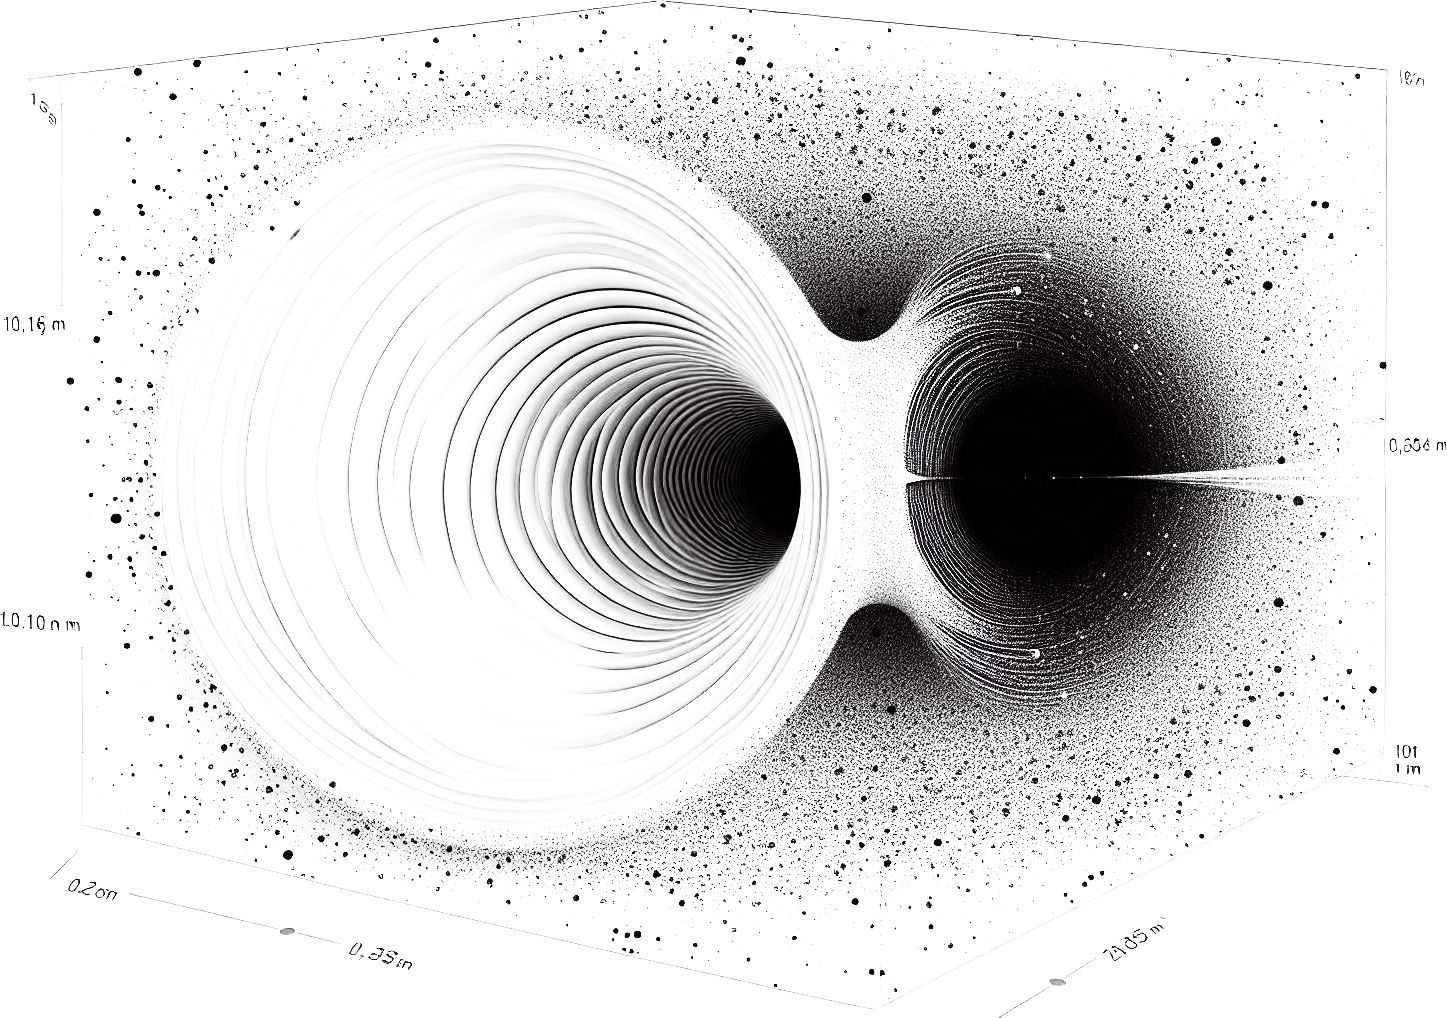
\includegraphics[width=0.6\linewidth]{OIG28.ZNLJ.PNG}
    \caption{%
     \footnotesize\textit{Representation of two interacting or connected funnel/tunnel-like geometries. The constituent lines suggest flow or field lines. In DUT, it could symbolize the interaction between two DUT black holes, a DUT wormhole-like connection, or a geometric visualization of quantum entanglement.}
    }
    \label{fig:Figura17}
\end{figure}

\subsubsection{Emergence of Lorentzian Signature}
\label{ssubsec:lorentz_sig_challenge_detailed}
\begin{itemize}
    \item \textbf{Problem:} The theory must dynamically explain why the emergent metric \( \langle \Op{g}_{\mu\nu} \rangle \) possesses a stable Lorentzian signature (+--- or -+++), rather than Euclidean (++++), especially if the fundamental structure does not presuppose it.
    \item \textbf{Implication:} Fundamental for recovering observed macroscopic physics.
    \item \textbf{Action (Phase 1d):} Analyze the spectral structure of the operator \( D_{\text{DUT}} \) and the emergent metric from the SAP. Investigate the role of quantum decoherence in selecting the signature (see \Cref{ssubsec:lorentz_sig_emergent_final_detailed}).
\end{itemize}

\subsection{Explicit Derivation from the Complete SAP ('Solution 0')}
\label{subsec:pae_derivation_detailed}

The heart of DUT lies in the SAP; its full implementation is the greatest computational and conceptual challenge.

\subsubsection{Effective Action and Fundamental Parameters ('Solution 0')}
\label{ssubsec:pae_derivation_challenge_detailed}
\begin{itemize}
    \item \textbf{Problem:} Perform the **explicit and complete derivation** of the low-energy effective action (\(\mathcal{L}_{EH}, \mathcal{L}_{SM}, \mathcal{L}_{\Psi_N}\) massive, and the form/coupling of \( \Op{\Theta}(\Op{\Psi}_N) \)) from the postulated SAP \( S = \Str_{\mathcal{H}}(f(D_{\text{DUT}}^2/\Lambda^2)) \). This requires constructing a plausible candidate \( D_{\text{DUT}} \) and calculating the heat kernel coefficients \( a_{2k} \) using the supertrace.
    \item \textbf{Implication:} Without this derivation, the theory's fundamental parameters (mass \( m_N \), self-coupling \( \lambda_{\text{eff}} \) of \( \Psi_N \), the coefficient \( \theta_0 \) of \( \Op{\Theta} \), SM constants, Planck mass \( M_{\text{Pl}} \)) are not determined from first principles, and the form of the potential \(V(\Psi_N)\) is unknown.
    \item \textbf{Proposed Strategy (Phase 2):} Follow the steps detailed in \Cref{ssubsec:pae_derivation_strategy_detailed}: define \( D_{\text{DUT}} \), calculate \(a_{2k}\) with Str, extract all terms of the effective action, confirming \( m_N \sim \Lambda \) and deriving \( \Op{\Theta} \).
\end{itemize}

\begin{figure}[htbp]
    \centering
    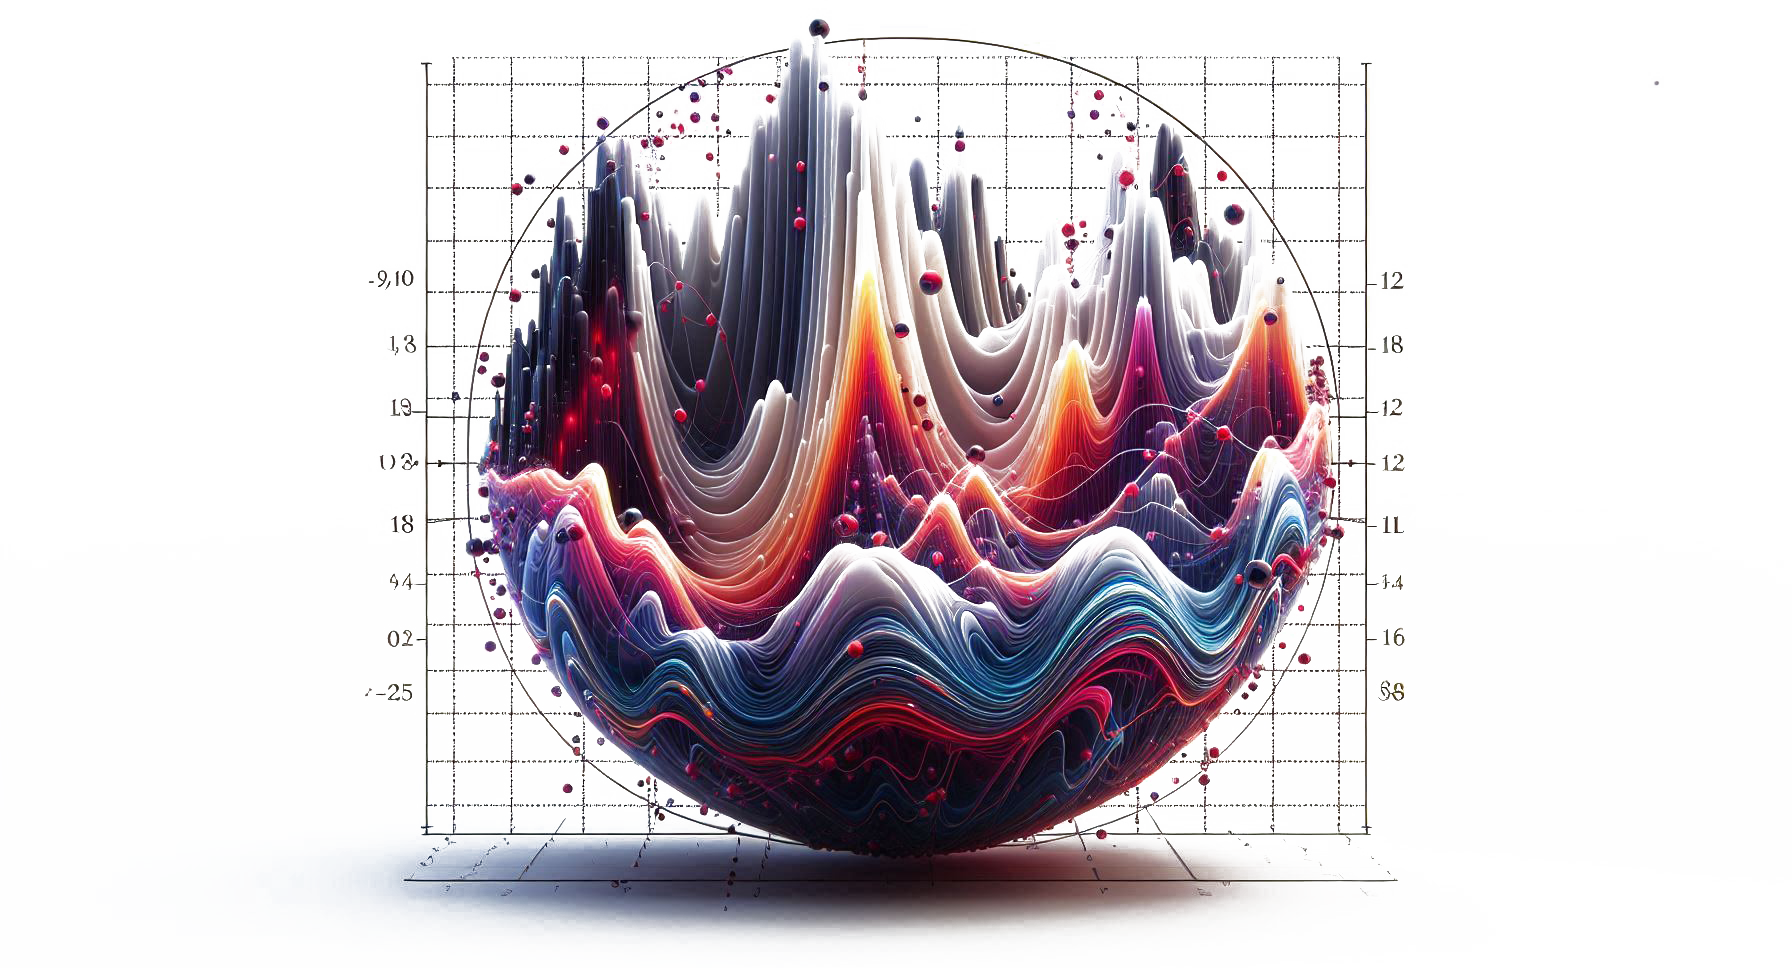
\includegraphics[width=0.6\linewidth]{OIG38.ZNLJ.PNG}
    \caption{%
     \footnotesize\textit{Realization of the explicit derivation from SAP of the effective action, including the justification of the potential \(V(\Psi_N)\) and the calculation of \(\Str_{\mathcal{H}}\).}
    }
    \label{fig:Figura19}
\end{figure}

\subsubsection{Cosmological Constant Cancellation via Supertrace}
\label{ssubsec:cc_cancel_challenge_detailed}
\begin{itemize}
    \item \textbf{Critical Problem:} Verify the fundamental CC cancellation hypothesis \( \Str_{\mathcal{H}}(f(D_{\text{DUT}}^2/\Lambda^2)) \approx 0 \) (\Cref{hyp:cc_cancel_final}). This demands not just postulating a symmetry (SUSY-like) but **explicitly demonstrating it** for the constructed \( D_{\text{DUT}} \) and calculating the resulting supertrace.
    \item \textbf{Implication:} If the supertrace does not vanish (or is not extremely small), DUT fails to solve the main CC problem, and its viability as a fundamental theory is compromised.
    \item \textbf{Action (High Priority, Phase 2b):} Once \( D_{\text{DUT}} \) is defined, perform the **explicit calculation of \( \Str_{\mathcal{H}} \)** for the \( a_0 \) term. Investigate whether a possible small residue could explain the observed DE.
\end{itemize}

\subsection{Hamiltonian Stability Analysis ('Solution 0')}
\label{subsec:hamiltonian_stability_analysis_detailed}

Ensuring the theory is physically stable is essential. The systematic approach includes:

\paragraph{1. Hamiltonian Formalism:} Derive the Hamiltonian \( \mathcal{H}_{\text{DUT}} \) from the effective Lagrangian \( \mathcal{L}_{\text{DUT}} \) ("Solution 0", \Cref{ssubsec:full_lagrangians_final_revised}) resulting from the SAP.

\paragraph{2. Constraint Analysis (Dirac-Bergmann):} Identify and classify all constraints (primary and secondary) to determine the physical degrees of freedom and verify the consistency of the formalism \citep{HenneauxTeitelboim1992}.

\paragraph{3. Linear Stability (Vacuum):} Analyze perturbations around the stable vacuum (\( \langle \Op{\Psi}_N \rangle = 0, \Theta = 0 \)). Given that \( m_N^2 > 0 \) and \( \lambda_{\text{eff}} > 0 \) are expected (see \Cref{teo:estabilidad_vacio} in appendix), and second-order Lagrangians, linear stability (absence of tachyons or linear ghosts) is anticipated.

\paragraph{4. Non-linear and Global Stability:} Investigate stability against large perturbations (e.g., via collapse simulations, \Cref{sec:collapse_TUD_ME}) and quantum vacuum stability (decay).

\paragraph{5. Stability of Emergent Gravity:} The modified Einstein-Grau equations:
\[
G_{\mu\nu} = 8\pi G_{\text{eff}} \left( T_{\mu\nu}^{\Psi_N} + T_{\mu\nu}^{\text{SM}} + \mathcal{O}(\Op{\Theta}^2) \right),
\]
are stable if the total effective energy-momentum tensor satisfies appropriate **energy conditions** (weak, strong, dominant). Since \( T_{\mu\nu}^{\Psi_N} \) derived from \( \mathcal{L}_{\Psi_N} \) with \(m_N^2>0, \lambda_{\text{eff}}>0\) fulfills these conditions (\Cref{ssubsec:full_lagrangians_final_revised}), stability in the \( \Op{\Theta} \to 0 \) limit is assured. It must be verified that the \( \mathcal{O}(\Op{\Theta}^2) \) corrections (to be derived from SAP) do not violate these conditions.

\paragraph{6. Verification of Absence of SAP Pathologies:} Confirm that the SAP expansion (especially \( a_4 \) with \( R^2 \dots \) terms) does not introduce ghost degrees of freedom with incorrect kinetic signs that compromise unitarity.

\paragraph{Conclusion on Stability (Phase 3a):} While "Solution 0" appears linearly stable, a full Hamiltonian analysis based on the SAP-derived action is required to confirm general stability and the absence of pathologies.

\subsection{Quantum Behavior and Renormalizability}
\label{subsec:quantum_behavior_detailed}
\begin{itemize}
    \item \textbf{Problem:} Analyze DUT's quantum structure. Is the theory renormalizable or just an effective theory? How does **UV/IR mixing** (\Cref{ssubsec:renormalization_final}) affect consistency and predictability, especially with dynamic \( \Op{\Theta} \)?
    \item \textbf{Implication:} Affects the theory's validity at arbitrarily high energies and its ability to solve the hierarchy problem.
    \item \textbf{Action (Phase 3b):} Investigate loop structure, potential cancellations or regularizations due to dynamic NCG, and the applicability of renormalization techniques for NC QFT \citep{GrosseWulkenhaar2005, Rivasseau:2010}.
\end{itemize}

\begin{figure}[htbp]
    \centering
    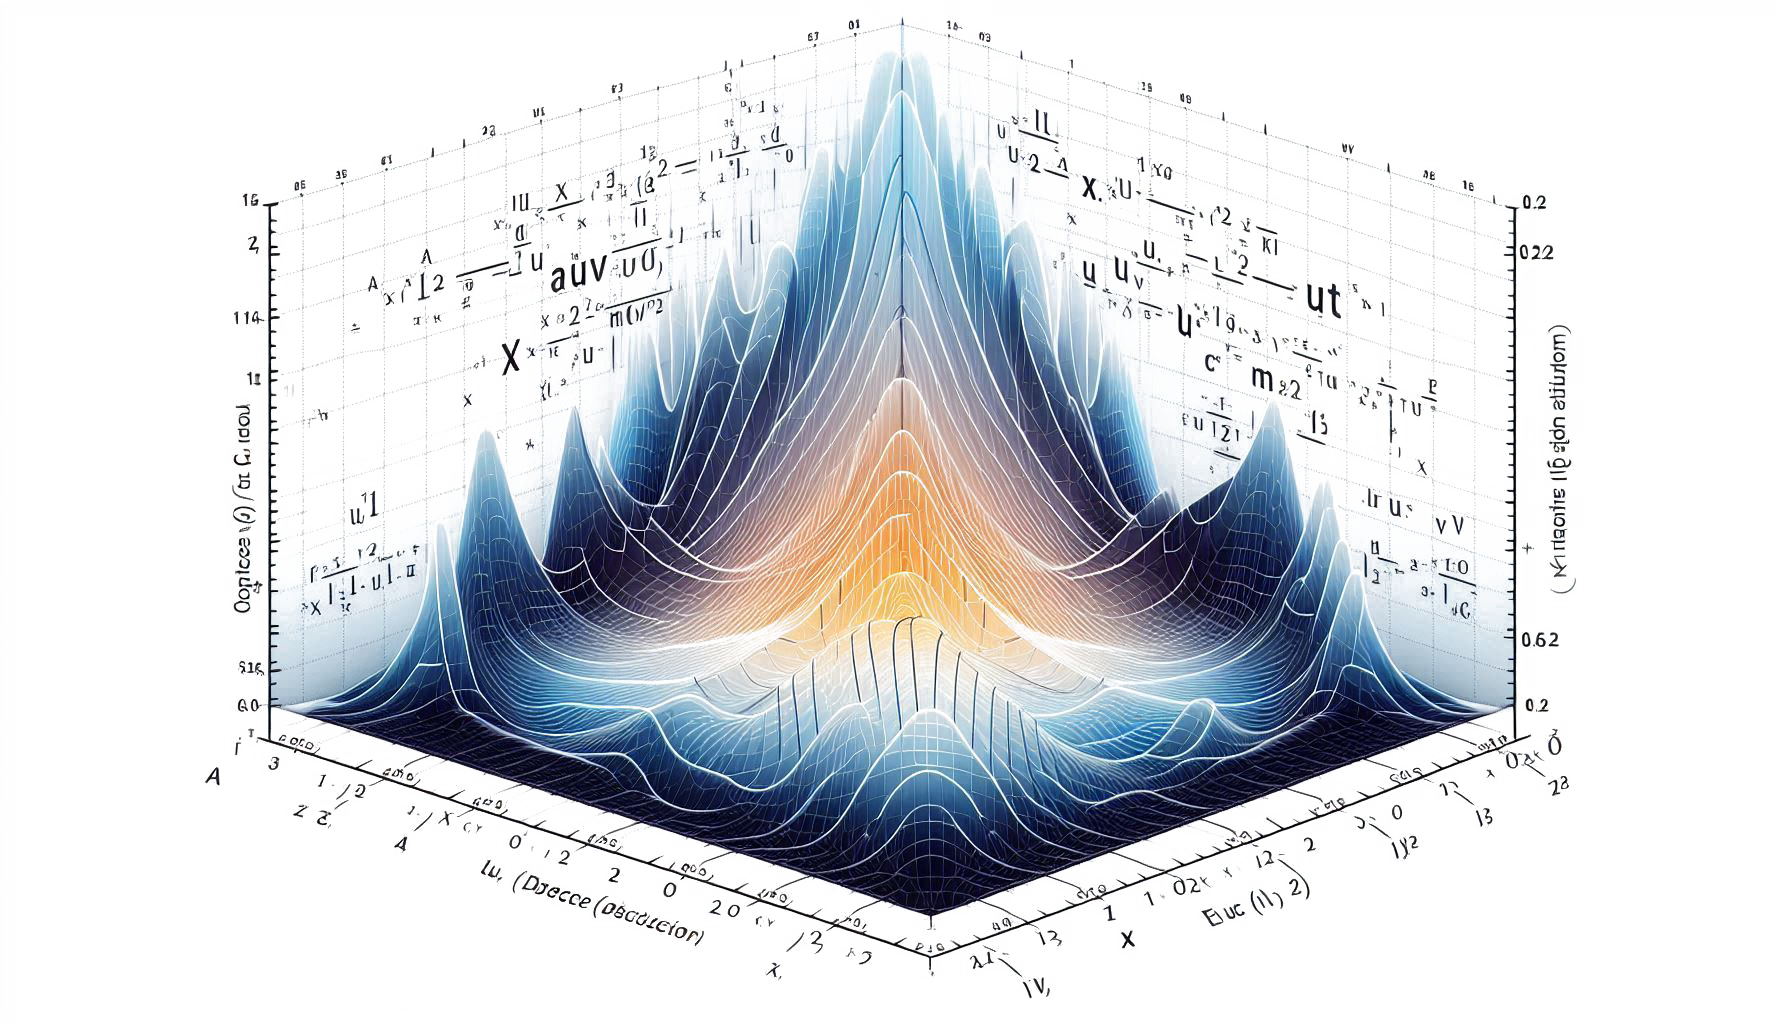
\includegraphics[width=0.6\linewidth]{OIG36.ZNLJ.PNG}
    \caption{%
     \footnotesize\textit{Abstract visualization related to energy scales or regularization, possibly illustrating how noncommutative structure might affect quantum corrections.}
    }
    \label{fig:Figura18}
\end{figure}

\subsection{Lack of Quantitative Calculations and Prioritized Roadmap ('Solution 0')}
\label{subsec:quantitative_roadmap_detailed}

DUT's main current weakness is the absence of quantitative results rigorously derived from its first principles. The following prioritized roadmap is proposed to systematically address the challenges and build the theory:

\begin{enumerate}[label=\textbf{Phase \arabic*}:, wide, labelwidth=!, labelindent=0pt, itemsep=2pt, topsep=3pt]
    \item \textbf{Foundations and Mathematical Consistency (High Priority):}
        \begin{enumerate}[label=\alph*), itemsep=1pt]
            \item Formalize a plausible candidate for the operator \( D_{\text{DUT}} \) (including structure for massive \( \Psi_N \) and generation of \( \Op{\Theta} \)).
            \item Explore the resulting functional form for \( \Op{\Theta}(\Op{\Psi}_N) \) emerging from couplings in \( D_{\text{DUT}} \).
            \item **Rigorously verify the Jacobi Identity** for this derived \( \Op{\Theta} \), ensuring \( \Star \) associativity (following \Cref{ssubsec:jacobi_resolution_strategy}).
            \item Analyze the dynamic emergence of the Lorentzian signature (\Cref{ssubsec:lorentz_sig_challenge_detailed}).
        \end{enumerate}
    \item \textbf{Base SAP Derivation (High Priority):}
        \begin{enumerate}[label=\alph*), itemsep=1pt]
            \item Calculate the heat kernel coefficients \( a_0, a_2, a_4 \) for \( D_{\text{DUT}} \) **using the supertrace (\( \Str \))**.
            \item **Verify the cancellation hypothesis \( a_0 \approx 0 \) (\( \Str_{\mathcal{H}} \approx 0 \))**. Analyze the magnitude and nature of any potential residue as a possible explanation (or not) for DE.
            \item Extract the complete effective action: \( \mathcal{L}_{EH} \) (verify \( M_{\text{Pl}} \)), \( \mathcal{L}_{SM} \) (verify standard couplings), \( \mathcal{L}_{\Psi_N} \) (**confirm \( m_N \sim \Lambda > 0 \)**, obtain \( \lambda_{\text{eff}} \)), and the explicit form and coefficient of \( \Op{\Theta}(\Op{\Psi}_N) \).
        \end{enumerate}
    \item \textbf{Stability and Quantization (Medium Priority):}
        \begin{enumerate}[label=\alph*), itemsep=1pt]
            \item Perform the full Hamiltonian analysis of the action derived in Phase 2 (\Cref{subsec:hamiltonian_stability_analysis_detailed}). Confirm linear and non-linear stability (complement with simulations).
            \item Initiate the study of the quantum structure: renormalizability, UV/IR effects with dynamic \( \Op{\Theta} \) (\Cref{subsec:quantum_behavior_detailed}).
        \end{enumerate}
    \item \textbf{Base Phenomenology (Dependent on Phases 1-3):}
        \begin{enumerate}[label=\alph*), itemsep=1pt]
            \item Calculate quantitative predictions for dynamic LIV (\Cref{subsec:liv_specific_final_revised}) based on the derived \( \Op{\Theta} \).
            \item Explore cosmological implications of heavy \( \Psi_N \) (role in inflation?, PBH formation?, defects as DM?). Calculate \( P(k) \) and \( f_{NL} \).
            \item Calculate corrections to QNMs (\Cref{ssubsec:nc_gw_qnm}) based on dynamic \( \Op{\Theta} \) in collapse/merger scenarios.
            \item Compare predictions with observational and experimental data.
        \end{enumerate}
    \item \textbf{Extensions (If Necessary):} If Phase 2b shows \( \Str_{\mathcal{H}} \approx 0 \) but the residue does not explain DE, explore justified extensions to \( D_{\text{DUT}} \) / SAP that could generate DE without introducing inconsistencies.
\end{enumerate}
This roadmap prioritizes establishing mathematical consistency and deriving the base physical structure of "Solution 0" before fully addressing detailed phenomenology or potential extensions.

\section{Conclusion}
\label{sec:conclusion_final_shifted}

\hrule
This document has presented a unified, detailed, and critically analyzed version of the base framework "Solution 0" of the Discrete Unification Theory (DUT). DUT proposes to unify General Relativity and the Standard Model via a Noncommutative Geometry (NCG) that emerges dynamically from 'spacetime nuclei' \( \Op{\Psi}_N \). The NCG is dynamic (\( \Op{\Theta}(\Op{\Psi}_N) \)) and the vacuum is postulated to be commutative (\( \langle \Op{\Theta} \rangle = 0 \)). Dynamics derive from the Spectral Action Principle (SAP) using the supertrace (\( \Str \)).

The "Solution 0" framework focuses on the direct consequences of this minimal structure. A key implication, based on expectations from the SAP, is that the fundamental field \( \Op{\Psi}_N \) is **massive** (\(m_N \sim \Mpl\)). This means that observed **Dark Energy** is **not explained by \( \Op{\Psi}_N \) quintessence** in this base version. Its explanation within DUT would depend on a **residue from the Cosmological Constant cancellation** (via the hypothesis \( \Str_{\mathcal{H}} \approx 0 \)) or would require **extensions** to the minimal SAP framework. Despite this limitation regarding DE, the base DUT framework maintains conceptual proposals to address Dark Matter (NC axions / defects of heavy \( \Psi_N \)), the **early formation of SMBHs** (relevant to JWST observations), the hierarchy problem (dynamic NC regularization), and the information paradox (NC correlations), as well as a unique prediction of **dynamic LIV** (consistent with current limits and testable).

The main contribution of this detailed version is the **explicit articulation of the fundamental theoretical challenges and the concrete strategies** proposed to address them (\Cref{sec:challenges_detailed}):
\begin{itemize}
    \item The imperative need to demonstrate the **mathematical consistency** of dynamic NCG, by deriving a form of \( \Op{\Theta}(\Op{\Psi}_N) \) compatible with the SAP that satisfies the Jacobi identity (\Cref{ssubsec:jacobi_resolution_strategy}).
    \item The central requirement to perform the **explicit derivation from the complete SAP** (\( S = \Str_{\mathcal{H}}(f(D_{\text{DUT}}^2/\Lambda^2)) \)), which includes:
        \begin{itemize}
            \item The **crucial verification of the CC cancellation hypothesis** (\( \Str_{\mathcal{H}} \approx 0 \)).
            \item The confirmation of the emergence of GR, SM, and a massive \( \Op{\Psi}_N \).
            \item The derivation of the functional form and coefficient of \( \Op{\Theta}(\Op{\Psi}_N) \).
        \end{itemize}
    \item The verification of complete **Hamiltonian stability** (\Cref{subsec:hamiltonian_stability_analysis_detailed}).
    \item The analysis of **quantum behavior** (renormalizability, UV/IR).
\end{itemize}
A **prioritized roadmap** (\Cref{subsec:quantitative_roadmap_detailed}) has been presented to guide future development, focused on first establishing mathematical consistency and deriving the base structure.

In conclusion, DUT ("Solution 0" Detailed and Complete) constitutes a **research program** that, while ambitious and facing formidable theoretical challenges, now possesses a clearer and internally coherent base conceptual framework, along with a defined work plan to validate (or refute) its fundamental postulates. The viability of DUT as a complete physical theory critically depends on the successful execution of the derivations, proofs, and calculations proposed in the roadmap. Future precision observations mentioned (\Cref{subsec:summary_validation_predictions_revised}) will be key to testing DUT's unique predictions, once they are quantitatively derived.

\bigskip
\hrule

\vfill
\begin{figure}[htbp]
    \centering
    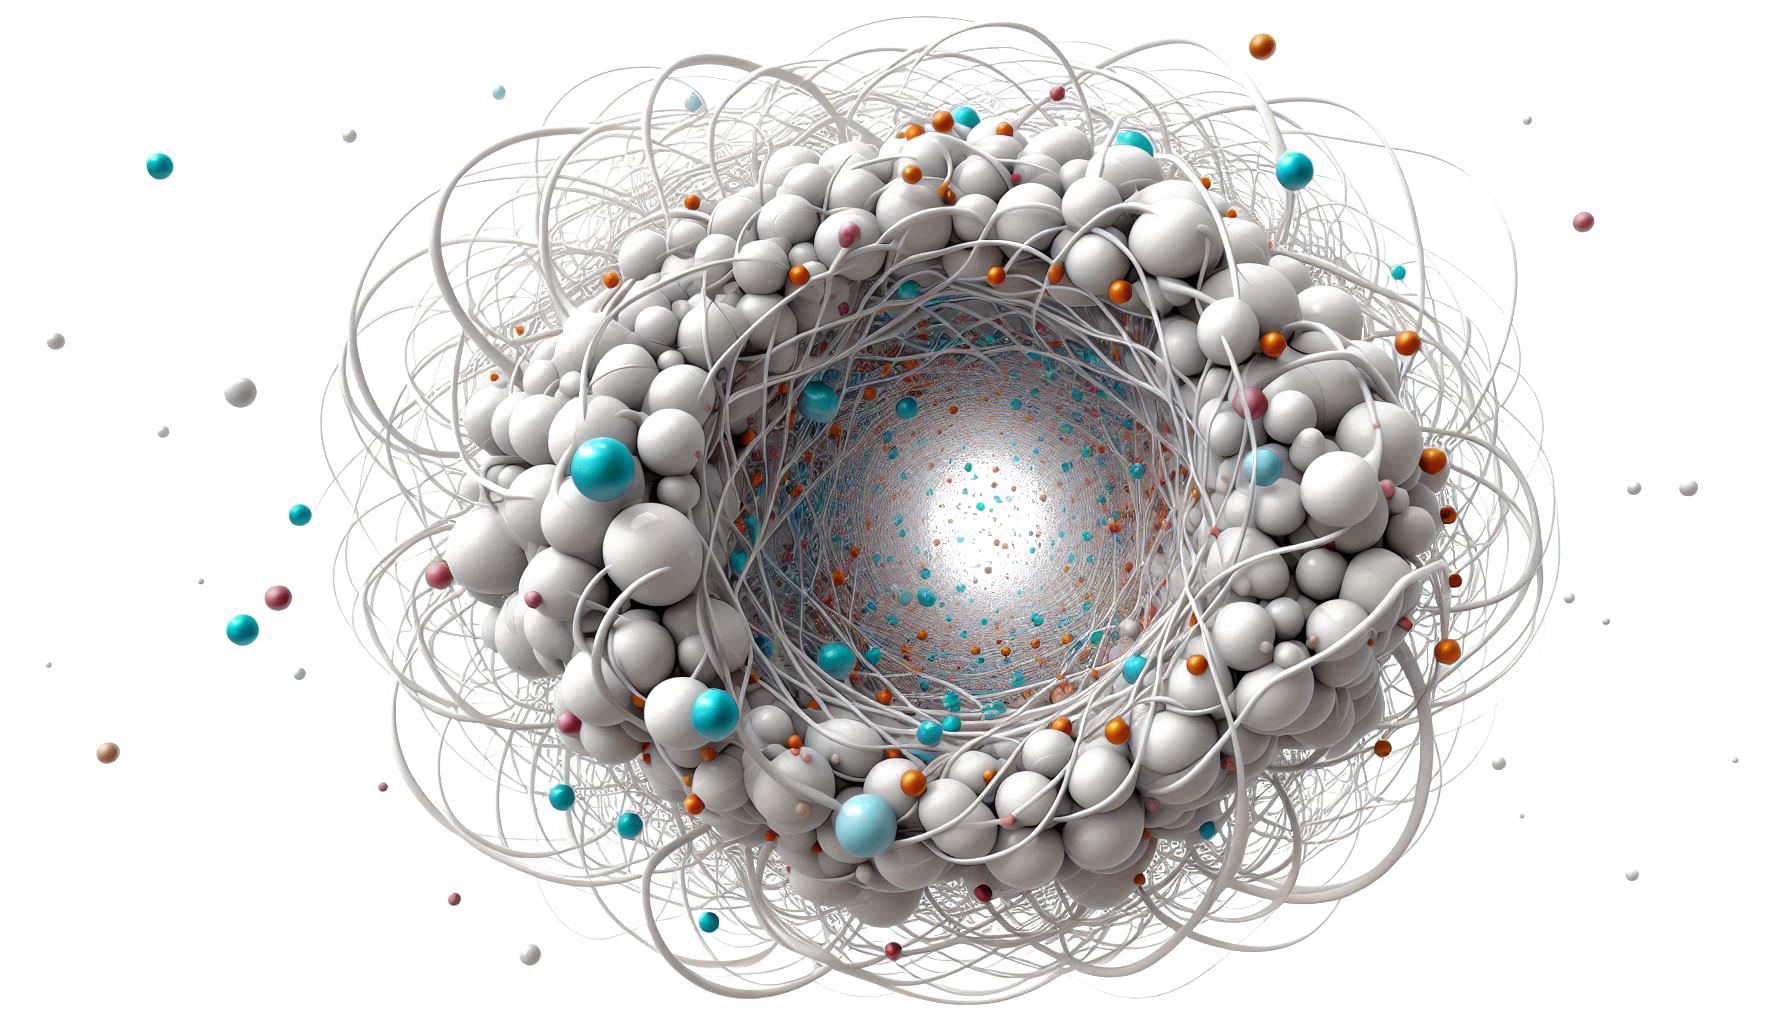
\includegraphics[width=0.9\linewidth]{OIG39.ZNLJ.PNG}
    \caption{%
     \footnotesize\textit{Representation of nuclei (\(\protect\Op{\Psi}_N\)).}
    }
    \label{fig:Figura20}
\end{figure}
\vfill
\bigskip
\hrule
\vfill


\appendix

\section{Mathematical Appendix}
\label{sec:apendice_matematico}

This section collects technical results and points for further investigation mentioned in the main text.

\subsection{Technical Lemma and Theorem}

\begin{lemma}[Approximate Dynamic Jacobi Identity]
\label{apendice:lema_jacobi}
Let \( \Op{\Theta}^{\mu\nu} = \theta_0 \, \partial^{[\mu} \Op{\Psi}_N (\star d\Op{\Psi}_N)^{\nu]} \). If \( \Op{\Psi}_N \) satisfies the equation of motion \( \Box \Op{\Psi}_N + V'(\Op{\Psi}_N) = 0 \), where \( V'(\Op{\Psi}_N) = m_N^2 \Op{\Psi}_N + \lambda_{\text{eff}} \Op{\Psi}_N^3 \), then the associated Schouten-Nijenhuis bracket \( [\Op{\Theta}, \Op{\Theta}]_{\text{SN}} \), which controls the Jacobi identity, is given by:
\[
[\Op{\Theta}, \Op{\Theta}]_{\text{SN}}^{\lambda\mu\nu} = \mathcal{O}(\Op{\Theta}^3) + C \theta_0^2 \lambda_{\text{eff}} \epsilon^{\dots[\lambda\mu\nu]\dots} \Op{\Psi}_N^2 (\partial \Op{\Psi}_N)^3 + \dots
\]
where \( C \) is a numerical constant. The Jacobi identity is satisfied exactly for the free field \( \lambda_{\text{eff}} = 0 \). For the interacting case, consistency requires the SAP to generate a form of \( \Op{\Theta} \) that satisfies it exactly, possibly needing additional terms as discussed in \cref{ssubsec:associativity_final}.
\end{lemma}

\begin{theorem}[Linear Stability of the Vacuum]
\label{teo:estabilidad_vacio}
The vacuum of DUT "Solution 0", characterized by \( \langle \Op{\Psi}_N \rangle = 0 \) and \( \langle \Op{\Theta}^{\mu\nu} \rangle = 0 \), is linearly stable against small perturbations \( \delta \Op{\Psi}_N \) if the mass parameter derived from the SAP satisfies \( m_N^2 > 0 \).
\end{theorem}
\begin{proof}[Proof]
Linearizing the equation of motion for \( \Op{\Psi}_N \) (\cref{eq:L_PsiN_explicit_final_redux}, \cref{eq:potencial_psi_n_final_redux}) around the vacuum \( \Op{\Psi}_N = 0 \), one obtains \( (\Box + m_N^2)\delta \Op{\Psi}_N = 0 \). Plane wave solutions \( \delta \Op{\Psi}_N \sim e^{ikx} \) satisfy the dispersion relation \( k^2 + m_N^2 = 0 \), or \( \omega^2 - |\vec{k}|^2 = m_N^2 \). If \( m_N^2 > 0 \), the frequencies \( \omega \) are real for all \( \vec{k} \), indicating stable oscillations without exponential growth (tachyons).
\end{proof}

\subsection{Points for Further Investigation}

1.  **Poisson Geometry and Deformation Quantization**
    * Explicit construction of \( \star \)-products associated with \( \Op{\Theta}(\Op{\Psi}_N) \) using the Kontsevich formula \citep{Kontsevich2003Deformation}.
    * Classification of possible Poisson structures in 4D that can be dynamically generated by \( \Op{\Psi}_N \).

2.  **Spectral Theory of Unbounded Operators**
    * Rigorous definition of the domain of the operator \( D_{\text{DUT}} \) on the Hilbert space \( \mathcal{H} \).
    * Analysis of the spectrum (discrete/continuous) of \( D_{\text{DUT}} \) and \( D_{\text{DUT}}^2 \), and how it depends on \( \Op{\Psi}_N \) excitations (via \( \Op{\Theta} \)).

3.  **Renormalization on Noncommutative Spaces**
    * Detailed analysis of Feynman diagrams in the emergent NC QFT of DUT.
    * Study of potential cancellation or modification of UV/IR divergences due to the dynamic nature of \( \Op{\Theta} \) \citep{GrosseWulkenhaar2005}.
    * Application of the Renormalization Group formalism to the effective action \( \mathcal{L}_{\text{DUT}} \).


\section{Goal: Derivation of SAP from First Principles}
\label{sec:apendice_pae_principios}

The ultimate validation of the Discrete Unification Theory (DUT) through the Spectral Action Principle (SAP) aims to rely **exclusively on first principles**, avoiding *ad hoc* assumptions or manual parameter adjustments. The goal is for all low-energy physics to emerge directly from the postulated fundamental mathematical structure. Below, we describe how this self-sufficient derivation is sought.

\subsection{Construction of \( D_{\text{DUT}} \) from the Fundamental Structure}
The starting point is the definition of the generalized Dirac operator \( D_{\text{DUT}} \) from the geometric and algebraic structure postulated for DUT, without manually introducing free parameters not justified by said structure.

\subsubsection{Fundamental Components (Non *Ad Hoc*)}
\begin{enumerate}
    \item \textbf{Dynamic Noncommutative Geometry (NCG):}
        A noncommutative algebra \( \mathcal{A} \) is postulated, generated by coordinate operators \( \hat{X}^\mu \) satisfying the fundamental relation (\Cref{eq:conmutador_nc_final}):
        \[
        [\hat{X}^\mu, \hat{X}^\nu]_\star = iM_{\text{Pl}}^{-2} \hat{\Theta}^{\mu\nu}(\Psi_N).
        \]
        Here, \( \hat{\Theta}^{\mu\nu} \) is not an external input but must be an operator field emerging dynamically, determined by the fundamental degrees of freedom \( \Psi_N \).

    \item \textbf{Generalized Dirac Operator \( D_{\text{DUT}} \):}
        \( D_{\text{DUT}} \) is sought to be constructed such that it faithfully represents the action of the algebra \( \mathcal{A} \) on the total Hilbert space \( \mathcal{H} \) of the theory (which includes spin, internal SM degrees of freedom, and \( \Psi_N \)). A general form could be \( D_{\text{DUT}} = i\gamma^\mu \nabla_\mu^{\text{NC}} + \mathcal{M}(\Psi_N, H, ...) \), where the noncommutative connection \( \nabla_\mu^{\text{NC}} \) and the mass/coupling term \( \mathcal{M} \) are dictated by the structure \( (\mathcal{A}, \mathcal{H}) \) and its symmetries, not by *ad hoc* adjustments. For example, \( \nabla_\mu^{\text{NC}} \) would include the spin connection and SM gauge fields coupled consistently with the \( \star \) product, and \( \mathcal{M} \) would contain terms generating Yukawa couplings and masses through interaction with the Higgs \( H \) and, crucially, the proper dynamics of \( \Psi_N \).
\end{enumerate}

\subsection{Calculation of the Effective Action without Arbitrary Assumptions}
The spectral action \( S = \text{Str}(f(D_{\text{DUT}}^2/\Lambda^2)) \) expands asymptotically. The goal is for the coefficients \( a_{2k} \) of this expansion to generate all known physics and the new physics of DUT without needing manual parameter fixing.

\subsubsection{Heat Kernel Coefficients (\(a_{2k}\))}
\begin{enumerate}
    \item **\(a_0\) - Sought Cancellation of the Cosmological Constant:**
        \[
        a_0 \propto \int_M \sqrt{g} \, \text{Str}(\mathbb{I}) \, d^4x.
        \]
        It is postulated (Hypothesis \Cref{hyp:cc_cancel_final}) that the structure of the total Hilbert space \( \mathcal{H} \) (including all bosonic and fermionic degrees of freedom) and the operator \( D_{\text{DUT}} \) possess a spectral symmetry such that the total supertrace vanishes: \( \text{Str}(\mathbb{I}) = \text{Tr}_{\mathcal{H}_B}(\mathbb{I}) - \text{Tr}_{\mathcal{H}_F}(\mathbb{I}) \approx 0 \). This cancellation, if verified by explicit calculation for the specific \( D_{\text{DUT}} \) of DUT, would eliminate the main \( \sim \Lambda^4 \) contribution to the CC. It does not necessarily require explicit SUSY, but the appropriate spectral balance. **Verifying this cancellation is a central goal (Phase 2b).**

    \item **\(a_2\) - Expected Emergence of Gravity and \( \Psi_N \) Mass:**
        \[
        a_2 \propto \int_M \sqrt{g} \, \text{Str}\left( c_1 R \cdot \mathbb{I} + c_2 (\nabla \Psi_N)^2 + c_3 m_N^2 \Psi_N^2 + \dots \right) d^4x.
        \]
        This term is expected to generate the Einstein-Hilbert action (\( \sim R \)) and the base dynamics of \( \Psi_N \).
        The objective is for the mass \( m_N \) to emerge proportionally to the fundamental scale \( \Lambda \) (\( m_N^2 \sim \Lambda^2 \), Hypothesis \Cref{hyp:psi_n_final}), and for the Planck constant \( M_{\text{Pl}} \) to be related to \( \Lambda \) and the spectral trace \( \text{Str}(\mathbb{I}_{\text{grav}}) \) over the relevant gravitational degrees of freedom, for example:
        \[
        M_{\text{Pl}}^2 \sim \frac{f_1}{f_0} \Lambda^2 \, \text{Str}(\mathbb{I}_{\text{grav}}) \quad (\text{if } f_0 \neq 0).
        \]
        **Confirming \( m_N \sim \Lambda \) and deriving \( M_{Pl} \) are key objectives (Phase 2c).**

    \item **\(a_4\) - Expected Emergence of Couplings and Noncommutativity:**
        \[
        a_4 \propto \int_M \sqrt{g} \, \text{Str}\left( C_{\mu\nu\rho\sigma}^2 + F_{\mu\nu}^2 + \lambda_{\text{eff}} \Psi_N^4 + \text{Yukawas} + \text{NC Terms} + \dots \right) d^4x.
        \]
        This term must generate the Yang-Mills actions for gauge fields \( F_{\mu\nu}^2 \), the Higgs potential and \( \Psi_N \) self-interactions (\( \sim \Psi_N^4 \)), Yukawa couplings, and crucially, the **terms defining the functional form and dynamics of the noncommutativity tensor \( \Op{\Theta}^{\mu\nu}(\Psi_N) \)**. \( \Op{\Theta} \) is expected to emerge from terms involving commutators of the type \( [D_{\text{DUT}}, \hat{X}^\mu]_\star \), making it intrinsically dynamic. **Explicitly deriving \( \Op{\Theta}(\Psi_N) \) and \( \lambda_{eff} \) is a central goal (Phase 2c).**
\end{enumerate}

\subsection{Consistency of Dynamic NCG from SAP}
The mathematical consistency of the noncommutative algebra, particularly the associativity of the \( \star \) product (which requires \( \Theta^{\mu\nu} \) to satisfy the Jacobi identity), must not be imposed externally but **must be a consequence of the dynamics derived from the SAP**.

\begin{enumerate}
    \item \textit{Consistency Requirement (Jacobi Identity):} For \( (f \star g) \star h = f \star (g \star h) \) to hold, the tensor \( \Op{\Theta}^{\mu\nu}(\Psi_N) \) emerging from the SAP calculation (\(a_4\), etc.) must satisfy the Jacobi identity (\( [\Theta, \Theta]_{\text{SN}} = 0 \)) or its quantum analogue.
    \item \textit{Emergence from Dynamics (Goal):} The aim is to demonstrate that the spectral action \( S = \text{Str}(...) \), when varied to obtain the complete equations of motion (EOMs) for all fields (including \( \Psi_N \)), generates a form for \( \Op{\Theta}(\Psi_N) \) and dynamics such that the Jacobi identity is automatically satisfied as a consistency condition. Although simple forms (like \( \Theta \propto \partial \Psi \wedge \partial \Psi \)) may not satisfy it if \( \Psi_N \) interacts (see Lemma \ref{apendice:lema_jacobi}), the complete form of \( \Theta \) derived from the SAP is required to do so. **Verifying this consistent emergence is a key challenge (Phase 1c), as discussed in \Cref{ssubsec:jacobi_resolution_strategy}.**
\end{enumerate}
Thus, associativity would be a consequence of the unified SAP dynamics, not an *ad hoc* assumption.

\subsection{Sought Emergence of Observed Physics}
\begin{enumerate}
    \item \textbf{General Relativity (GR):} Must emerge from \( a_2 \), with \( M_{\text{Pl}} \) spectrally determined by \( \Lambda \).
    \item \textbf{Standard Model (SM):} All its fields, gauge groups, and representations must be encoded in the initial choice of \( (\mathcal{A}, \mathcal{H}, D_{\text{DUT}}) \). Gauge, Higgs, and Yukawa couplings must emerge from the \( a_2 \) and \( a_4 \) coefficients with values related to spectral traces over internal degrees of freedom (e.g., \( g_A^{-2} \propto \text{Str}(T_A^2) \), \( m_f \propto y_f \propto \text{Str}(Y_f...) \)).
    \item \textbf{Dark Energy (DE):} If the cancellation \( \text{Str}(\mathbb{I}) \approx 0 \) is not exact at the quantum level (due to loop corrections), the resulting residue \( \delta \Lambda^4 \) is a potential candidate to explain the observed DE. However, demonstrating that this residue has the correct magnitude (\( \sim (10^{-3} \text{eV})^4 \)) without fine-tuning requires a full NC QFT calculation and is a significant challenge.
\end{enumerate}

\subsection{Sought Consistency Checks (Without *Ad Hoc* Elements)}
The following table summarizes how key elements of the theory are expected to be determined by the formalism itself:

\begin{table}[h!]
\centering
\footnotesize
\begin{tabularx}{\textwidth}{@{}lX@{}}
\toprule
\textbf{Aspect}             & \textbf{Expected Mechanism in DUT (Requires Verification)} \\
\midrule
**Mass of \( \Psi_N \)** & Determined by \( a_2 \): \( m_N^2 \sim \Lambda^2 \). Not manually adjusted (Verify in Phase 2c). \\ \addlinespace
**SM Constants** & Fixed by symmetries of \( \mathcal{A} \), structure of \( \mathcal{H} \), and spectral traces in \( a_2, a_4 \) (Derive explicitly in Phase 2c). \\ \addlinespace
**CC \(\rho_{vac}\) Cancellation** & Sought result of \( \text{Str}(\mathbb{I}) \approx 0 \), expected consequence of balanced spectral structure of \( (\mathcal{H}, D_{\text{DUT}}) \) (Verify in Phase 2b). \\ \addlinespace
**Noncommutativity \( \Theta^{\mu\nu} \)** & Dynamic field \( \Op{\Theta}(\Psi_N) \) whose form and dynamics emerge from \( a_4 \) and EOMs (Derive in Phase 2c, verify Jacobi consistency in Phase 1c). \\
\bottomrule
\end{tabularx}
\caption{Summary of the sought non *ad hoc* origin for DUT components.}
\label{tab:non_ad_hoc_summary}
\end{table}

\subsection{Conclusion of the Goal}
The goal of the SAP validation program in DUT is to achieve a **self-contained and predictive derivation from first principles**. If successful:
\begin{itemize}
    \item Geometry, fundamental fields (\(\Psi_N\)), SM fields, and all physical constants (masses, couplings, \(M_{Pl}\)) would emerge from the initial spectral structure \( (\mathcal{A}, \mathcal{H}, D_{\text{DUT}}) \) and the scale \( \Lambda \).
    \item There would be no *ad hoc* adjustable free parameters in the fundamental action; everything would be determined by the SAP dynamics.
    \item Mathematical consistency (associativity \( \star \), Jacobi identity for \( \Theta \)) would be a verifiable consequence of the unified equations of motion.
\end{itemize}
Achieving this goal would make DUT a **highly predictive and falsifiable** fundamental theory, where observable physics would be a direct consequence of the initial mathematical choice of the spectral triple \( (\mathcal{A}, \mathcal{H}, D_{\text{DUT}}) \). The success of the research program outlined in the roadmap (\Cref{subsec:quantitative_roadmap_detailed}) will determine if this goal is attainable.

\section{References}
\label{sec:references_final}

\bibliographystyle{unsrtnat}
\bibliography{bibliography/references}

\end{document}




